
\documentclass{article} % For LaTeX2e
\usepackage{iclr2026_conference,times}

% Optional math commands from https://github.com/goodfeli/dlbook_notation.
\input{math_commands.tex}

\usepackage{hyperref}
\hypersetup{colorlinks=true,linkcolor=blue,citecolor=blue,urlcolor=blue}
\usepackage{url}
\usepackage{amsmath,amssymb,amsthm}
\usepackage{algorithm}
\usepackage{graphicx}
\usepackage{booktabs}
\usepackage{subcaption}
\usepackage{enumitem}
\usepackage{bbm}

\newtheorem{theorem}{Theorem}
\newtheorem{lemma}[theorem]{Lemma}
\newtheorem{proposition}[theorem]{Proposition}
\newtheorem{corollary}[theorem]{Corollary}
\newtheorem{definition}{Definition}
\newtheorem{remark}{Remark}
\newtheorem{assumption}{Assumption}
\newtheorem{example}{Example}
\newtheorem{conjecture}{Conjecture}
\newtheorem*{theorem*}{Theorem}
\newtheorem*{lemma*}{Lemma}
\newtheorem*{proposition*}{Proposition}
\newtheorem*{corollary*}{Corollary}
\newtheorem*{remark*}{Remark}
\newcommand{\zach}[1]{{\color{blue}#1}}

\title{Hyper-Ridge PersonalEvo: Meta-Learning the Archive Geometry for Provable Personalized Routing}
% Authors must not appear in the submitted version. They should be hidden
% as long as the \iclrfinalcopy macro remains commented out below.
% Non-anonymous submissions will be rejected without review.

\author{Anonymous Authors}

% The \author macro works with any number of authors. There are two commands
% used to separate the names and addresses of multiple authors: \And and \AND.
%
% Using \And between authors leaves it to \LaTeX{} to determine where to break
% the lines. Using \AND forces a linebreak at that point. So, if \LaTeX{}
% puts 3 of 4 authors names on the first line, and the last on the second
% line, try using \AND instead of \And before the third author name.

\newcommand{\fix}{\marginpar{FIX}}
\newcommand{\new}{\marginpar{NEW}}
\providecommand{\R}{\mathbb{R}}
\providecommand{\E}{\mathbb{E}}
\providecommand{\argmax}{\mathop{\mathrm{arg\,max}}\limits}
\providecommand{\argmin}{\mathop{\mathrm{arg\,min}}\limits}
\providecommand{\D}{\mathcal{D}}
\providecommand{\Aq}{\mathcal{A}_q}
\providecommand{\simplex}{\Delta_K}
\providecommand{\Risk}{R}
\providecommand{\eRisk}{\widehat{R}}
\providecommand{\KL}{\mathrm{KL}}
\providecommand{\ip}[2]{\langle #1,\, #2\rangle}
\providecommand{\Qcal}{\mathcal{Q}}
\providecommand{\Pcal}{\mathcal{P}}
\providecommand{\Fcal}{\mathcal{F}}
\providecommand{\VC}{\mathrm{VC}}
\providecommand{\dhat}{\widehat{\delta}}
\providecommand{\phat}{\widehat{p}}
\providecommand{\Mhat}{\widehat{M}}
\providecommand{\what}{\widehat{w}}
\providecommand{\wstar}{w^{\star}}
\providecommand{\sign}{\mathrm{sign}}
\providecommand{\Too}{\widetilde{O}}
\providecommand{\solid}{\textsc{[solid]}}
\providecommand{\needsproof}{\textsc{[needs-proof]}}

%\iclrfinalcopy % Uncomment for camera-ready version, but NOT for submission.

% Definitions harvested from the source documents' preambles
\usepackage{mathtools}
\usepackage{algpseudocode}
\providecommand{\calA}{\mathcal{A}}
\usepackage{multirow}
\providecommand{\zz}[1]{\textcolor{blue}{(zz: #1)}}
\providecommand{\hl}[1]{\textcolor{red}{#1}}
\providecommand{\Rstatic}{V_{\mathrm{static}}}
\providecommand{\Droute}{\Delta_{\mathrm{route}}}
\providecommand{\deff}{d_{\mathrm{eff}}}
\providecommand{\Err}{\mathrm{Err}}
\providecommand{\Kmax}{K_{\max}}
\begin{document}
\allowdisplaybreaks[3]

\maketitle

% \paragraph{Base paper.}
% \emph{PersonalEvo: Provable Personalized Routing for Self-Evolving Agents.}

% \paragraph{Motivating paper.}
% \emph{Meta-Learning with Generalized Ridge Regression: High-dimensional
% Asymptotics, Optimality and Hyper-covariance Estimation.}

\begin{abstract}
Personalized agents maintain libraries of prompt variants, skill modules, or orchestration policies, which we call \emph{candidates}, collected in an \emph{archive}.

The simplest strategy is \emph{uniform deployment}: pick the single candidate with the highest average reward across all users.

We propose PersonalEvo, a contextual-bandit method that learns to route each user to their best-matching candidate online, and optionally grows the archive by evolving new candidates after failures.

We give PersonalEvo a provable guarantee: its reward decomposes exactly into four interpretable terms, the \emph{default reward} of the best single candidate served to everyone, a \emph{routing gain} $\Delta_{\mathrm{route}}$ from matching each user to their own best candidate, an \emph{evolution gain} from newly discovered candidates, and an \emph{exploration cost} paid while learning user preferences.

This decomposition yields a sharp condition for when personalization helps, routing provably outperforms uniform deployment whenever the routing and evolution gains together exceed the exploration cost, together with a plug-in regret bound on the exploration cost.

We evaluate PersonalEvo on nine benchmarks: three synthetic personalized-agent environments, two agent-framework substrates (GEPA prompt archives \citep{agrawal2025geparp}, Hermes skill configurations \citep{hermes_selfevolution}), and four real-data preference datasets (BESPOKE \citep{personalized_agent_pabf}, PAHF Shopping and Embodied \citep{pahf2025}, and PrefEval \citep{zhao2025prefeval}).

Across all nine, PersonalEvo achieves higher mean reward than both the static baseline and random candidate selection.

Our results show that: (1)~the routing gain $\Delta_{\mathrm{route}}$ is larger than the evolution gain on every benchmark; (2)~on the four real-data benchmarks, $\Delta_{\mathrm{route}}$ ranges from $0.036$ to $0.251$, indicating that the value of personalized routing varies substantially across application domains; (3)~growing the archive without gating hurts performance, because the added observed-reward residual outweighs the evolution gain. The saved base experiments report \(m_t-r_t\), not the mean-reward exploration cost \(m_t-\mu(U,a_t)\) in our theorem.

Building on this base, we introduce \emph{Hyper-Ridge PersonalEvo}, which replaces independent isotropic regularization with a shared archive geometry. For known geometry, we prove a pathwise exploration bound with an explicit confidence radius and an effective-dimension potential term. We also prove finite-sample covariance control for a calibration-split variant that estimates the geometry from fresh candidates and freezes it before routing. With fixed problem constants, its explicit calibration charge and width-inflation remainder are $o(\sqrt{T})$, while its full exploration bound is $O(\sqrt{T}\log T)$. Neither theorem covers the periodically re-estimated router. In diagnostics, the true geometry lowers cumulative exploration cost by $46$--$59\%$, whereas periodic re-estimation raises it by $7$--$19\%$.
\end{abstract}

\section{Introduction}

\label{sec:intro}

Modern LLM agents increasingly choose among collections of prompts, skills, tools, and workflows instead of relying on one fixed policy. We call such a collection an \emph{archive} and each deployable entry a \emph{candidate}. Personalization methods learn user profiles and preference-conditioned behavior \citep{salemi2023lamp,zhao2025prefeval,personalized_agent_pabf}; prompt and agent evolution methods search for stronger candidates \citep{fernando2023promptbreeder,guo2024evoprompt,zhou2024symbolic,agrawal2025geparp}; and routing methods choose among available models or policies at inference time \citep{ong2024routellm,hu2024routerbench,li2025llmbandit,tsai2026neuralucb}. These lines of work address three related decisions: what a user prefers, how the archive should improve, and which candidate should handle the next request.

Consider a support agent whose archive contains formal and casual policies for refund and shipping requests. This example fixes the setting we study. At each round a user arrives, the agent deploys one candidate from the current archive, and only the deployed candidate's reward is observed; candidate selection is therefore a contextual bandit over the archive. The agent is also self-evolving: after poor feedback it mutates an existing candidate and adds the result to the archive, so the set of arms grows during deployment. Serving every user the best policy on average discards the archive's useful diversity. A personalized router can learn which policy works for each user, but it must first try candidates whose value is uncertain. Archive growth makes this cost recur: each new mutation is a new arm that a conventional bandit starts learning from scratch. Yet the candidates are related. What the router learns about formality from a refund policy should inform a formal shipping policy, even though the two policies should retain different reward models. Archive growth therefore creates a tension: it can add better candidates while also adding enough exploration to erase their benefit.

Existing methods resolve only parts of this tension. Profile and memory methods condition an agent on the user, but do not control exploration over a growing archive \citep{salemi2023lamp,personalized_agent_pabf,zhang2025personaagent,westhausser2025persistent}. Evolution methods improve candidate quality, usually offline or at the population level, but do not learn which candidate to serve to each user online \citep{fernando2023promptbreeder,guo2024evoprompt,zhou2024symbolic,agrawal2025geparp}. Fixed-pool routers make that assignment, but do not account for archive growth \citep{ong2024routellm,li2025llmbandit,tsai2026neuralucb}. Standard disjoint linear bandits also estimate every candidate independently, so evidence about one candidate cannot reduce uncertainty about another \citep{li2010contextual,chu2011linucb}. Pooling all candidates into one predictor goes too far in the other direction and erases real candidate-specific differences. What is missing is the \emph{geometry of variation across the archive}: which behavioral directions recur across candidates, which differences remain candidate-specific, and when evidence can be transferred between them.

These observations lead to the question studied in this paper:
\begin{quote}
\emph{Can a self-evolving agent transfer evidence across related archive candidates while retaining a measurable guarantee that personalized routing is worth its exploration cost?}
\end{quote}

We address this question in two steps. First, \emph{PersonalEvo} separates the value of personalization from the cost of learning it. Let $A_1$ be the initial archive and let $R_T$ be the router's average reward over $T$ interactions. We prove the exact decomposition
\begin{equation}
\label{eq:intro-decomp}
R_T
\,=\,
V_{\mathrm{static}}(A_1)
+
\Delta_{\mathrm{route}}(A_1)
+
\bar G_T
-
\bar L_T ,
\end{equation}
where $V_{\mathrm{static}}(A_1)$ is the reward from serving everyone the best single initial candidate, $\Delta_{\mathrm{route}}(A_1)$ is the gain from matching users to different initial candidates, $\bar G_T$ is the gain from candidates discovered after deployment, and $\bar L_T$ is the reward lost while the router learns. In the support example, these terms are the best universal reply policy, the value of matching tone and topic to each user, the value of newly evolved replies, and the cost of trying the wrong reply. The identity holds for any measurable router and gives the testable deployment criterion
\begin{equation}
\label{eq:intro-dominance}
\Delta_{\mathrm{route}}(A_1) + \bar G_T \,>\, \bar L_T ,
\end{equation}
so personalized routing is worthwhile exactly when its routing and evolution gains cover its exploration cost.

Second, \emph{Hyper-Ridge PersonalEvo} targets the only negative term in \eqref{eq:intro-decomp}. Each candidate $a$ has its own parameter vector $\theta_a$, which maps $d$ user and candidate features to expected reward. A disjoint LinUCB router estimates each vector with the same spherical regularizer and therefore encodes no relation among candidates \citep{abbasi2011oful,chu2011linucb}. We instead model the candidate vectors as draws with a shared covariance $\Omega$. This covariance is the archive geometry. Its dominant directions capture recurring factors such as tone and topic, while every candidate keeps its own reward model. Hyper-Ridge uses this geometry to regularize candidate estimates, so a newly evolved candidate starts with uncertainty shaped by the archive rather than an isotropic blank slate.

The gain is largest when candidate parameters vary mainly along a few shared directions even though the feature representation is high-dimensional. Let $\bar d_{\mathrm{eff},T}(\Omega)$ be a deterministic upper bound on the effective dimension of every candidate design through round $T$, and let $c_T^\Omega=1+\log(1+TL_\Omega^2/\lambda)$. For known $\Omega$, our theorem gives the explicit exploration budget
\begin{equation}
\label{eq:intro-hyper-cost}
B_T^\Omega(\delta)
=
2\alpha_{\Omega,T}(\delta)
\sqrt{2K_{\max}T\,c_T^\Omega\bar d_{\mathrm{eff},T}(\Omega)},
\end{equation}
where $\alpha_{\Omega,T}(\delta)$ is the confidence radius stated in Proposition~\ref{prop:deff-bound}. The base LinUCB budget has the same form with its own radius and the isotropic potential $d\log(1+TL_x^2/(\lambda d))$. Thus geometry helps only when the complete budget in \eqref{eq:intro-hyper-cost}, including its confidence radius, is smaller. For $T\ge2$, with fixed problem parameters and $\delta=1/T$, both valid noisy-reward bounds scale as $O(\sqrt{T}\log T)$; the benefit is in their problem-dependent geometric factors, not a missing logarithm. The calibration-split theorem retains an estimated-geometry confidence radius; its separate calibration charge and width-inflation remainder are $o(\sqrt{T})$. It does not cover the periodically updated estimator in Algorithm~\ref{alg:hyper-ridge}.

Our experiments separate the motivation for Hyper-Ridge from evidence for its mechanism. Across nine benchmarks, the base PersonalEvo router has routing gains from $0.036$ to $0.280$, evolution gains from $0$ to $0.061$, and observed-reward residuals from $0.010$ to $0.071$. Because the simulator clips noisy rewards, these residuals are not identified with the theorem's mean-reward exploration cost. On separate planted rank-three problems, giving Hyper-Ridge the true geometry lowers cumulative exploration cost by $46$--$59\%$. Periodically estimating that geometry instead raises the cost by $7$--$19\%$. On seven adapter benchmarks, one-hot candidate features make the full-covariance router identical to its diagonal ablation, so their reward changes cannot show cross-candidate transfer. The evidence therefore supports the known-geometry mechanism while exposing the unresolved estimation and representation problem.

\paragraph{Contributions.}
This paper makes four contributions:
\begin{enumerate}
\item \textbf{A measurable formulation of personalized self-evolution.} We formalize routing over a growing candidate archive and prove the exact four-term decomposition \eqref{eq:intro-decomp}, which turns the decision to personalize into the testable criterion \eqref{eq:intro-dominance}.
\item \textbf{Archive-aware routing.} We introduce Hyper-Ridge PersonalEvo, which learns a covariance geometry across candidate reward models and uses it in a generalized-ridge UCB router. It shares evidence about important feature directions while retaining candidate-specific predictions.
\item \textbf{Effective-dimension guarantees with a clear boundary.} We prove a known-$\Omega$ bound with its full confidence radius and a finite-sample calibration-split theorem for estimated $\Omega$. We do not transfer either guarantee to the unresolved periodic estimator.
\item \textbf{Evidence that separates mechanism from implementation.} We measure the structural terms and report the logged observed-reward residual on nine benchmarks, then test Hyper-Ridge in a controlled low-rank setting. The results show when the right geometry helps and why the current periodic estimator and one-hot representation do not yet realize that gain.
\end{enumerate}

\paragraph{Paper organization.}
Section~\ref{sec:related} positions the work relative to personalization, agent evolution, routing, and linear bandits. Section~\ref{sec:background} defines the routing problem and Hyper-Ridge estimator. Section~\ref{sec:theory} develops the decomposition and effective-dimension analysis. Section~\ref{sec:experiments} reports the base-router results, Hyper-Ridge diagnostics, and remaining evaluation gap. Appendix~\ref{app:hyper-proofs} proves the oracle geometry results, and Appendix~\ref{app:err-control-proof} gives the calibration-split covariance theorem.

\section{Related Work}

\label{sec:related}

Routing queries across a model or prompt pool to trade off cost and quality is now standard: RouteLLM \citep{ong2024routellm} learns a strong/weak router from preference data and RouterBench \citep{hu2024routerbench} benchmarks such routers, while LLM Bandit \citep{li2025llmbandit} and NeuralUCB routing \citep{tsai2026neuralucb} cast routing as an online contextual bandit.

These route at the \emph{model} level over a fixed pool; PersonalEvo routes \emph{per user} over an archive that may grow online, and decomposes the resulting reward rather than only reporting it.

Benchmarks such as LaMP \citep{salemi2023lamp}, PersonalLLM \citep{zollo2024personalllm}, and PrefEval \citep{zhao2025prefeval} supply user-feedback signals, while PersonaAgent \citep{zhang2025personaagent} and persistent-memory frameworks \citep{westhausser2025persistent} maintain per-user personas and evolving profiles.

The closest personalized-bandit antecedent, PAB-F \citep{personalized_agent_pabf}, models per-user reward as a factorized function of context and a fixed memory/tool/style action set, and studies regret against an in-archive oracle.

Prompt and agent evolution methods, including Promptbreeder \citep{fernando2023promptbreeder}, EvoPrompt \citep{guo2024evoprompt}, Symbolic Learning \citep{zhou2024symbolic}, and GEPA's reflective Pareto search \citep{agrawal2025geparp}, improve prompts or archives through offline search rather than online user-conditioned routing.

Hermes self-evolution \citep{hermes_selfevolution,hermes_agent} adds constraint-gated growth, which motivates our archive-growth gate.

Classical contextual-bandit methods such as OFUL and LinUCB \citep{abbasi2011oful,chu2011linucb,li2010contextual} provide standard finite-time tools for controlling exploration in linear bandits, and related structural-vs-online decompositions appear in contextual pricing, offline RL, and multi-task transfer.

\section{Preliminaries: PersonalEvo Routing and the Hyper-Ridge Estimator}
\label{sec:background}

\label{sec:method}

\subsection{Overview}

\label{sec:method-plain}
Managed platforms such as Microsoft Foundry Agent Service and Amazon Bedrock AgentCore \citep{microsoft2026foundryagents,aws2026agentcore} let teams build and deploy agents from models, tools, and instructions. A product team can maintain several agent configurations---for example, different system prompts or tool policies---and revise them as feedback arrives. We use these products only as concrete deployment settings; neither is assumed to implement our router.

A personalized agent keeps a small library, an \emph{archive}, of candidate prompts, skills, or routing templates.

At each round, it receives one user's request, picks one candidate from the current archive, observes a reward for that candidate, updates its state, and may add an evolved child to the archive.

We compare this personalized routing policy with a no-adaptation baseline: pick the candidate in the initial archive with the highest population-mean reward and use it for every user and every round. A comparator that picks again each round is a dynamic selection policy; it would fold online learning or archive growth into the baseline. Fixing one initial candidate lets us measure routing gain, evolution gain, and exploration cost separately.

The remainder of this section formalizes the notation, introduces the hyper-ridge estimator and its generalized-ridge model, presents the routing algorithm, and states the base theoretical results.

\subsection{Notation and setup}

\label{sec:method-notation}
Prompt evolution is one concrete instance of this loop. A task supplies an input to an LLM system with a system prompt; the system's output is scored or receives textual feedback; and an optimizer such as GEPA \citep{agrawal2025geparp} uses that feedback to propose and test a revised prompt. We call each deployable version a \emph{candidate}. More generally, candidates may differ in their prompts, tool configurations, model choices, or agent policies. Evolution determines which candidates enter the archive, while routing determines which available candidate serves a particular user. We ask whether this per-user choice earns enough reward to cover the cost of learning user preferences.

A user $U \sim \Pi$ is drawn from a population: $\mathcal{U}$ denotes the user space (in our benchmarks a finite set of user profiles; in general an abstract measurable space), and $\Pi$ is a probability distribution over $\mathcal{U}$, so $\Pi$ is not a vector or matrix and has no dimension of its own; it simply specifies how likely each user is to arrive. Practically, $\Pi$ is the deployment's user mix, and expectations $\E_U[\cdot]$ below average over that mix.

The system operates over $T \in \mathbb{N}$ rounds (successive requests) and starts from a deterministic initial archive $A_1$ shared by all users. This finite set is $A_1 = \{a^{(1)}, \dots, a^{(K)}\}$, where each $a$ is one deployable unit of agent behavior and $K = |A_1|$. Evolution may enlarge the archive along user $U$'s trajectory, so $A_t(U)$ denotes the archive available to that user at round $t$, with $|A_t(U)| \leq K_{\max}$. We use $A$ without a subscript or user argument only for an arbitrary fixed archive in definitions such as $V_{\mathrm{static}}(A)$.

The analysis follows \emph{one} user's trajectory and then averages over the population. A single user \(U\) is drawn once and interacts with the system for \(T\) rounds. Let \(\mathcal O_{t-1}\) be the router's observable pre-action history: the user, the initial archive, all earlier actions and rewards, and the archive available at round \(t\). For concentration arguments, let \(\mathcal F_{t-1}\supseteq\mathcal O_{t-1}\) be an analysis filtration that also contains latent candidate parameters and proposer randomness once they are generated. The router's action is \(\mathcal O_{t-1}\)-measurable; enlarging the filtration for the proof does not give the router access to those latent variables. Population-level statements then average over \(U\) and all online randomness. Quantities with argument \(U\), such as \(A_t(U)\), \(a_t(U)\), \(G_t(U)\), and \(L_t(U)\), are per-user random variables.  Quantities with an expectation or a bar, such as \(V_{\mathrm{static}}\), \(V_{\mathrm{route}}\), \(\bar G_T\), \(\bar L_T\), and \(R_T\), are population averages.

At round $t$, the user-specific archive $A_t(U)$ is available to the router and is required to be $\mathcal{O}_{t-1}$-measurable.

The router selects $a_t(U) \in A_t(U)$ and observes the reward
\begin{equation}
r_t \,=\, \mu(U, a_t(U)) + \xi_t ,
\end{equation}
Here \(r_t\) is the scalar feedback generated when user \(U\) receives candidate \(a_t(U)\). Conditional on the user, archive construction, and latent candidate parameters, its remaining randomness is the observation noise \(\xi_t\), with \(\E[\xi_t\mid\mathcal F_{t-1}]=0\). Unconditional statements may also average over proposer randomness and the random-effects model introduced below. The function \(\mu(u,a)\in[0,1]\) is the noise-free mean reward of serving candidate \(a\) to user \(u\).

The current-archive oracle value is $m_t(U) = \max_{a \in A_t(U)} \mu(U,a)$.

We define the four terms of \eqref{eq:method-thesis}.

The \emph{default reward} is $V_{\mathrm{static}}(A) \,=\, \max_{a \in A} \E_{U}[\mu(U,a)]$: average each candidate's reward over all users \emph{first}, then pick the single best candidate and serve it to everyone. This is the performance of the simplest possible deployment, one that does no personalization at all (a single fixed prompt or policy shipped to every user), so it is the operating point a team is already at before adopting any routing method; it is the baseline any personalization system must beat to justify its cost.

The \emph{oracle routing value} is $V_{\mathrm{route}}(A) \,=\, \E_{U}[\max_{a \in A} \mu(U,a)]$, with the two operations in the opposite order: for \emph{each} user pick that user's best candidate first, then average over users. This is the ceiling of personalization, the reward if user preferences were known perfectly and no exploration were ever needed. Practically it answers a question a team should ask before building anything: ``if personalization worked perfectly on this archive, how much would we earn?'' No online algorithm on the fixed archive can exceed it.

Their difference is the \emph{routing gain} $\Delta_{\mathrm{route}}(A) \,=\, V_{\mathrm{route}}(A) - V_{\mathrm{static}}(A) \,\geq\, 0$: the reward gained by matching candidates to users instead of shipping one candidate to everyone. For a self-evolving archive, our four-term decomposition separates this structural gain from the gain due to archive growth and the online cost of learning which candidate to choose. Thus $\Delta_{\mathrm{route}}(A)$ is the reward budget available to pay for personalization. If users are nearly homogeneous, or one candidate dominates for everyone, then $\Delta_{\mathrm{route}}(A) \approx 0$ and user-specific routing offers little benefit. If some users prefer concise replies while others prefer detailed explanations, $\Delta_{\mathrm{route}}(A)$ can be large. A team can estimate this quantity on held-out users before deployment and compare it with the expected exploration cost.

These quantities say \emph{why} personalization matters but not \emph{when} it pays off; the dominance condition of Corollary~\ref{cor:dominance} answers the latter by weighing $\Delta_{\mathrm{route}}$ against the exploration cost.

The \emph{evolution gain} at round $t$ is $G_t(U) \,=\, m_t(U) - m_1(U)$, measuring how much the archive has improved since initialization. We define it because self-modification is not free (each mutation adds an arm the router must explore), so a deployment needs to know how much reward the newly evolved candidates are actually adding; $G_t(U)$ is exactly that amount, the improvement of the best-available candidate for user $U$ between round $1$ and round $t$. It is measured by bookkeeping, not by extra experiments: whenever a candidate is added, evaluate the incumbent best and the new candidate for the affected user and record the difference of the two bests. Concretely, in the support-archive example: if user $U$'s best launch-day template has mean satisfaction $m_1(U) = 0.70$ and at round $t$ a mutated template raised the best available to $m_t(U) = 0.78$, then $G_t(U) = 0.08$; if evolution never produced anything better for this user, $G_t(U) = 0$. In our simulators $\mu$ is known so $m_t(U)$ is computed exactly; in a live system it is estimated by scoring the current archive on the user's held-out interactions.

The \emph{exploration cost} is $L_t(U) \,=\, m_t(U) - \mu(U, a_t(U))$, the gap between the current-archive best and what the router actually picked. It is the price of learning and the only negative term in the decomposition. Continuing the same example, if the best current template has mean satisfaction $0.78$ but the router serves one with mean $0.60$, that round costs $0.18$. The simulator contains both means needed to compute this quantity, but the saved headline tables use \(m_t-r_t\) instead. A live system must estimate both means on held-out or logged interactions and report the resulting uncertainty separately.


The horizon-averaged terms are $\bar G_T \,=\, \frac{1}{T}\sum_{t=1}^T \E[G_t(U)]$ and $\bar L_T \,=\, \frac{1}{T}\sum_{t=1}^T \E[L_t(U)]$.

\subsection{Model}
\label{sec:method-model}

For the Hyper-Ridge theory, write the bounded mean reward as

\begin{equation}
\mu(u,a)=b(u)+x(u,a)^\top\theta_a ,
\end{equation}
where $x(u,a)\in\mathbb{R}^d$ is the user-candidate feature vector and the known baseline $b(u)$ is common to every candidate offered to user $u$. We assume $\mu(u,a)\in[0,1]$. A convenient compatible model is $b(u)=1/2$ and $x(u,a)^\top\theta_a\in[-1/2,1/2]$.

Instead of estimating each $\theta_a$ with ordinary ridge regression, assume
the candidate parameters are random effects:

\begin{equation}
\mathbb{E}[\theta_a]=0,\qquad
\mathbb{E}[\theta_a\theta_a^\top]=\Omega,
\end{equation}
where $\Omega \in \mathbb{R}^{d \times d}$ is a hyper-covariance matrix shared
across archive candidates. The common baseline makes this zero-mean random-effects model compatible with nonnegative rewards. It also cancels from every candidate comparison.

The goal is to estimate $\Omega$ from the archive and use it to regularize
routing.

\subsection{Hyper-ridge estimator}

For candidate $a$, define

\begin{equation}
X_{a,t} = \bigl[ x_s^\top \bigr]_{s < t : a_s = a}, \qquad
y_{a,t} = (r_s-b(u_s))_{s < t : a_s = a}.
\end{equation}
Given an estimate $\widehat{\Omega}_t$, define the generalized ridge estimator

\begin{equation}
\widehat{\theta}_{a,t}
= \arg\min_{\theta \in \mathbb{R}^d}
\left\{ \| y_{a,t} - X_{a,t}\theta \|_2^2
      + \lambda \theta^\top \widehat{\Omega}_t^{-1} \theta \right\}.
\end{equation}
Equivalently,

\begin{equation}
\widehat{\theta}_{a,t}
= \left( X_{a,t}^\top X_{a,t} + \lambda \widehat{\Omega}_t^{-1} \right)^{-1}
  X_{a,t}^\top y_{a,t}.
\end{equation}
Define the generalized design matrix

\begin{equation}
V_{a,t}^{\mathrm{hyper}} = X_{a,t}^\top X_{a,t} + \lambda \widehat{\Omega}_t^{-1}.
\end{equation}
Then the Hyper-Ridge UCB score is

\begin{equation}
\mathrm{UCB}_t^{\mathrm{hyper}}(u, a)
= x(u, a)^\top \widehat{\theta}_{a,t}
+ \alpha \sqrt{ x(u, a)^\top \left( V_{a,t}^{\mathrm{hyper}} \right)^{-1} x(u, a) }.
\end{equation}
The selected candidate is

\begin{equation}
a_t(u) \in \arg\max_{a \in A_t(u)} \mathrm{UCB}_t^{\mathrm{hyper}}(u, a).
\end{equation}
\subsection{Algorithm}

\label{sec:method-alg}

Algorithm~\ref{alg:hyper-ridge} summarizes the resulting routing procedure.
It mirrors the base PersonalEvo router round for round; the only changes are
the generalized ridge geometry $\lambda \widehat{\Omega}_t^{-1}$ inside
$V_{a,t}^{\mathrm{hyper}}$ and the periodic re-estimation of the
hyper-covariance from the archive's own per-candidate estimates.

Three clarifications about the data the algorithm accumulates. First, $y_{a,t}$ stacks centered observed rewards $r_s-b(u_s)$, not unknown mean rewards. Second, row $s$ of $X_{a,t}$ is the feature vector for the user served at that round, so a shared router may pool observations from many users. Third, Algorithm~\ref{alg:hyper-ridge} allows a stream of users, whereas the four-term decomposition follows one user and then averages over the population. Whenever we combine a Hyper-Ridge bound with that decomposition, we use the per-user specialization $u_t\equiv U$. The confidence and potential lemmas also hold for a predictable user stream, but the four-term conclusion does not automatically transfer to that setting.

\begin{algorithm}[t]
\caption{Hyper-Ridge PersonalEvo routing}
\label{alg:hyper-ridge}
\begin{algorithmic}[1]
\Require Initial archive $A_1$, ridge weight $\lambda > 0$, exploration
  weight $\alpha > 0$, re-estimation period $\tau \in \mathbb{N}$,
  regularizer $\epsilon > 0$
\State Initialize $\widehat{\Omega}_1 \gets I_d$; for each candidate $a$,
  initialize $X_{a,1}$ and $y_{a,1}$ as empty
\For{$t = 1, 2, \dots, T$}
  \State Observe user $u_t$ and eligible candidate set $A_t(u_t)$
  \For{each candidate $a \in A_t(u_t)$}
    \State Compute
      $V_{a,t}^{\mathrm{hyper}} \gets X_{a,t}^\top X_{a,t}
        + \lambda \widehat{\Omega}_t^{-1}$
    \State Compute
      $\widehat{\theta}_{a,t} \gets
        \bigl( V_{a,t}^{\mathrm{hyper}} \bigr)^{-1}
        X_{a,t}^\top y_{a,t}$
    \State Compute
      $\mathrm{UCB}_t^{\mathrm{hyper}}(u_t, a) \gets
        x(u_t, a)^\top \widehat{\theta}_{a,t}
        + \alpha \sqrt{ x(u_t, a)^\top
          \bigl( V_{a,t}^{\mathrm{hyper}} \bigr)^{-1} x(u_t, a) }$
  \EndFor
  \State Select
    $a_t \in \arg\max_{a \in A_t(u_t)} \mathrm{UCB}_t^{\mathrm{hyper}}(u_t, a)$
    and observe reward $r_t$; set $y_t\gets r_t-b(u_t)$
  \State Update per-candidate data: append $x(u_t, a_t)^\top$ to
    $X_{a_t, t+1}$ and $y_t$ to $y_{a_t, t+1}$
  \If{$t \equiv 0 \pmod{\tau}$}
    \State Re-estimate the hyper-covariance from the archive's
      candidate estimates:
      \begin{equation}
        \widehat{\Omega}_{t+1} \gets
          \frac{1}{|A_t|} \sum_{a \in A_t}
          \widehat{\theta}_{a,t} \widehat{\theta}_{a,t}^\top
          + \epsilon I_d
      \end{equation}
  \Else
    \State $\widehat{\Omega}_{t+1} \gets \widehat{\Omega}_t$
  \EndIf
\EndFor
\end{algorithmic}
\end{algorithm}

The per-round cost is identical to base PersonalEvo up to the
re-estimation step, which touches only the $d \times d$ matrix
$\widehat{\Omega}_t$ and amortizes over the period $\tau$. This periodic update
is an experimental method. Proposition~\ref{prop:deff-bound} analyzes the
oracle variant that fixes $\widehat\Omega_t=\Omega$ and uses the stated
confidence radius. Theorem~\ref{thm:err-control-calibration-split-final}
analyzes a second variant that estimates $\Omega$ on independent calibration
candidates and freezes the estimate before routing. Neither result applies to
the periodic update above.

The remainder of the paper turns to empirical evidence. Section~\ref{sec:experiments}
first reports the nine-benchmark results for the base PersonalEvo router and
then separates two Hyper-Ridge questions: whether a known archive geometry can
reduce exploration, and whether the current periodic estimator can recover that
geometry from online data.


Algorithm~\ref{alg:router} describes PersonalEvo's per-user routing loop.

At each round, a disjoint LinUCB bandit selects the best candidate for the current user based on UCB scores.

In the simulator, an oracle-assisted gate compares the unknown current-archive optimum with the observed reward and may propose a new candidate.

\begin{algorithm}[t]
\caption{Per-user personalized routing over a growing archive.}
\label{alg:router}
\begin{algorithmic}[1]
\Require user $u$, common initial archive $A_1$, horizon $T$, exploration parameter $\alpha$, gap threshold $\tau$, cooldown $\kappa$, archive cap $K_{\max}$
\State $A_1(u) \gets A_1$; for each $a \in A_1(u)$ initialize $A_a \gets I$, $b_a \gets 0$
\State $t_{\mathrm{last}} \gets -\infty$
\For{$t = 1, \dots, T$}
    \For{each $a \in A_t(u)$}
        \State $x_t(a) \gets \psi(u,a)$ \Comment{feature map, \eqref{eq:method-feat}}
        \State $\hat\theta_a \gets A_a^{-1} b_a$
        \State $\mathrm{UCB}_t(a) \gets \hat\theta_a^\top x_t(a) + \alpha \sqrt{x_t(a)^\top A_a^{-1} x_t(a)}$
    \EndFor
    \State $a_t(u) \gets \arg\max_{a \in A_t(u)} \mathrm{UCB}_t(a)$
    \State observe $r_t = \mu(u, a_t(u)) + \xi_t$
    \State $A_{a_t(u)} \gets A_{a_t(u)} + x_t(a_t(u)) x_t(a_t(u))^\top$;\quad $b_{a_t(u)} \gets b_{a_t(u)} + r_t \, x_t(a_t(u))$
    \If{$m_t(u) - r_t > \tau$ \textbf{and} $t - t_{\mathrm{last}} > \kappa$ \textbf{and} $|A_t(u)| < K_{\max}$} \Comment{oracle-assisted gate}
        \State $\tilde a_t(u) \gets \mathcal{F}(u, A_t(u), \mathrm{trace}_t)$;\ \ $A_{t+1}(u) \gets A_t(u) \cup \{\tilde a_t(u)\}$;\ \ initialize $A_{\tilde a}, b_{\tilde a}$;\ \ $t_{\mathrm{last}} \gets t$
    \Else
        \State $A_{t+1}(u) \gets A_t(u)$
    \EndIf
\EndFor
\end{algorithmic}
\end{algorithm}

The feature map used in our experiments is

\begin{equation}
\label{eq:method-feat}
\psi(u,a) = \big[\,\mathrm{onehot}(\mathrm{cat}(a))\,;\, w_u\,\big] \in \mathbb{R}^{2K_{\mathrm{cat}}},
\end{equation}

where $\mathrm{cat}(a)$ is the candidate's category and $w_u \in \mathbb{R}^{K_{\mathrm{cat}}}$ is the user preference vector exposed by the simulator.

As a concrete instance (used in our experiments), the $K_{\mathrm{cat}}=5$ categories are $\{\text{sorting}, \text{searching}, \text{formatting}, \text{general}, \text{calc}\}$, so for a candidate $a$ in the \texttt{searching} category, $\mathrm{onehot}(\mathrm{cat}(a))=(0,1,0,0,0)$ and the user block $w_u$ records that user's affinity for each of the five categories.

We refer the reader to Appendix~\ref{app:implementation} for the full construction (categories, quality components, and feature concatenation), and to \citet{personalized_agent_pabf} for a richer factorized feature map over task type, memory mode, tool mode, and answer style.

The reflection trigger is the high-gap-failure rule

\begin{equation}
\label{eq:method-trigger}
m_t(u) - r_t > \tau,\qquad t - t_{\mathrm{last}} > \kappa,
\end{equation}

This gate is not deployable as written because $m_t(u)$ uses unknown mean rewards. The saved simulator also uses an oracle-assisted proposer: it reads the user's peak category and returns a child candidate biased toward that category.

The measured evolution gain therefore describes this idealized simulator. It is not a formal upper bound on a different proposer, and it does not show what an LLM-driven proposer would achieve.

\paragraph{Reward decomposition.}
Using Algorithm~\ref{alg:router}, we show that the average reward the router achieves over horizon $T$ satisfies (the subscript $1$ in $A_1$ refers to the round $t=1$ initial archive shared across all users, not to a particular user):

\begin{equation}
\label{eq:method-thesis}
\text{routed value}
\,=\, V_{\mathrm{static}}(A_1) + \Delta_{\mathrm{route}}(A_1) + \bar G_T - \bar L_T.
\end{equation}

This equation separates the router's performance into the four terms defined
above. Computing all four terms requires the current-archive optimum and the
selected candidate's mean reward; observed rewards alone are not enough.

\paragraph{Example.} Consider two candidates and two equally likely user types with means $\mu(u_1,a_1)=0.9$, $\mu(u_2,a_1)=0.4$, $\mu(u_1,a_2)=0.4$, $\mu(u_2,a_2)=0.9$.

Then $V_{\mathrm{static}}=0.65$ (the best single candidate averages $0.65$), while $V_{\mathrm{route}}=0.9$ (matching each user to their best gives $0.9$), so $\Delta_{\mathrm{route}}=0.25$.

With no archive growth ($\bar G_T=0$), the decomposition gives: routed value $= 0.65 + 0.25 - \bar L_T$.

Routing is profitable as long as the exploration cost $\bar L_T < 0.25$.

When a held-out reward model supplies \(\mu(u,a)\),
\(V_{\mathrm{static}}\) and \(\Delta_{\mathrm{route}}\) can be estimated from a
held-out user sample:
\(V_{\mathrm{static}}(A_1)=\max_a N^{-1}\sum_u\mu(u,a)\) and
\(\Delta_{\mathrm{route}}(A_1)
=N^{-1}\sum_u\max_a\mu(u,a)-V_{\mathrm{static}}(A_1)\).

Computing \(\bar G_T\) and \(\bar L_T\) also requires the archive means
\(m_t(u)\) and the selected mean \(\mu(u,a_t(u))\). The saved tables use
\(m_t(u)-r_t\) instead, which is a different observed-reward residual.

\section{Method}

The preceding sections establish the base PersonalEvo framework: a routing decomposition over a self-evolving archive, guarantees for the fixed-archive router, and a repair-time bound for archive growth. All of these results are inherited unchanged. In this section we introduce the revision's contribution: a replacement for the router's per-candidate estimation scheme, motivated by a meta-learning perspective on the archive. The new method leaves the decomposition and its first three terms intact and targets only the exploration-cost term, by importing hyper-covariance estimation ideas from generalized ridge regression. We first record the two source documents that anchor this revision.







\subsection{Summary of what changes}

Before turning to experiments, we summarize how this section modifies the base
paper. First, the router changes: the generalized-ridge router defined by
$V_{a,t}^{\mathrm{hyper}}$ and $\mathrm{UCB}_t^{\mathrm{hyper}}$ replaces the
base per-candidate LinUCB router, which regularizes each $\theta_a$
independently with an isotropic ridge penalty. Second, the exploration-cost
theory changes: the known-$\Omega$ theorem replaces the isotropic potential by
an effective-dimension potential while retaining the full confidence radius.
Appendix~\ref{app:err-control-proof} proves finite-sample control for a
calibration-split estimator that freezes $\widehat{\Omega}$ before routing.
The periodically updated estimator in Algorithm~\ref{alg:hyper-ridge} has no
guarantee in this paper. Geometry improves the certificate only when the full
Hyper-Ridge budget is smaller than the full LinUCB budget; low effective
dimension alone is not sufficient. Finally, nothing else changes: the
four-term decomposition
$R_T = \Rstatic(A_1) + \Droute(A_1) + \bar{G}_T - \bar{L}_T$ is inherited from
the base framework exactly as proven there, and this revision only sharpens
the bound on the $\bar{L}_T$ term.

\section{Theoretical Results for Hyper-Ridge PersonalEvo}
\label{sec:hyper-theory}



\subsection{Theory: improved exploration cost}

\label{sec:method-assump}

Throughout this section the base assumptions of Section~\ref{sec:background} (Assumptions~\ref{ass:bounded}--\ref{ass:bounded-feat} below) remain in force, and we write $x(u,a)$ for the feature map denoted $\psi(u,a)$ there; the only new hypothesis is the shared archive geometry of Assumption~\ref{assump:shared-structure}. We first restate the inherited base results this revision builds on, then derive the sharpened exploration-cost bound.

The decomposition holds under minimal conditions (bounded rewards and measurability).

Below we state the assumptions needed for the finite-time guarantee.

\begin{assumption}[Bounded mean reward]
\label{ass:bounded}
The mean reward is bounded:
\begin{equation}
\label{eq:ass-bounded}
\mu(u,a) \in [0,1] \quad \text{for all } (u,a).
\end{equation}
\end{assumption}

\begin{assumption}[Conditionally sub-Gaussian noise]
\label{ass:subg}
There exists $\sigma > 0$ with
\begin{equation}
\label{eq:ass-subg}
\E\!\left[\exp(\lambda \xi_t) \mid \mathcal{F}_{t-1}\right] \,\le\, \exp(\lambda^2 \sigma^2 / 2), \qquad \lambda \in \mathbb{R}.
\end{equation}
\end{assumption}

\begin{assumption}[Predictable archive]
\label{ass:predictable}
The user-specific archive is predictable:
\begin{equation}
\label{eq:ass-pred}
\sigma(A_t(U)) \subseteq \mathcal{O}_{t-1}.
\end{equation}
\end{assumption}

\begin{assumption}[Bounded features]
\label{ass:bounded-feat}
The feature map satisfies
\begin{equation}
\label{eq:ass-feat}
\|\psi(u,a)\| \,\le\, L < \infty \quad \text{for all } (u,a).
\end{equation}
\end{assumption}

Assumptions~\ref{ass:subg}--\ref{ass:bounded-feat} are not required for Theorem~\ref{thm:decomp} (the main result); they are needed only for the conditional plug-in corollary that imports an exploration-cost bound from the linear bandit literature.

\label{sec:method-lem-het}

The first result establishes when routing gain is strictly positive:

\begin{lemma}[Static-vs-routed value]
\label{lem:hetero}
For every finite archive $A$,
\begin{equation}
\label{eq:lem-hetero}
\Delta_{\mathrm{route}}(A) \,\ge\, 0,
\end{equation}
with equality if and only if there exists $a^\star \in A$ such that
\begin{equation}
\label{eq:lem-hetero-eq}
\mu(U, a^\star) = \max_{a \in A} \mu(U,a) \quad \text{almost surely.}
\end{equation}
\end{lemma}

Thus \(\Delta_{\mathrm{route}}(A)>0\) exactly when no single candidate is
optimal for almost every user.

The proof is in Appendix~\ref{app:proofs}.

\paragraph{Main theorem.}

\label{sec:method-thm-decomp}

\begin{theorem}[Exact decomposition on the common initial archive]
\label{thm:decomp}
Let $A_1$ be deterministic, finite, and shared by all users. For every round $t$ and every horizon $T \ge 1$,
\begin{equation}
\label{eq:thm-decomp-pointwise}
\E[\mu(U, a_t(U))]
\,=\, V_{\mathrm{static}}(A_1) + \Delta_{\mathrm{route}}(A_1) + \E[G_t(U)] - \E[L_t(U)].
\end{equation}
\begin{equation}
\label{eq:thm-decomp-avg}
\frac{1}{T}\sum_{t=1}^T \E[\mu(U, a_t(U))]
\,=\, V_{\mathrm{static}}(A_1) + \Delta_{\mathrm{route}}(A_1) + \bar G_T - \bar L_T.
\end{equation}
\end{theorem}

\begin{proof}[Proof sketch (full proof in Appendix~\ref{app:proofs})]
By definition,
\begin{equation*}
\begin{aligned}
\mu(U,a_t(U))
&\,=\,m_t(U)-L_t(U)\\
&\,=\,m_1(U)+G_t(U)-L_t(U).
\end{aligned}
\end{equation*}
Taking expectations over all model and online randomness and using
Lemma~\ref{lem:hetero} gives \eqref{eq:thm-decomp-pointwise}. Averaging over
$t$ gives \eqref{eq:thm-decomp-avg}.
\end{proof}

Theorem~\ref{thm:decomp} says that the reward achieved by the personalized routing policy decomposes into a structural piece on the initial archive ($V_{\mathrm{static}}+\Delta_{\mathrm{route}}$), an online discovery piece ($\bar G_T$), and a negative online learning piece ($-\bar L_T$).

In a simulator that logs mean rewards, \(\bar L_T\) is computed from
\(m_t(u)-\mu(u,a_t(u))\). The saved headline artifacts instead contain
\(m_t(u)-r_t\), so they do not directly measure \(\bar L_T\).

\paragraph{Dominance condition.}

\label{sec:method-cor-dom}

\begin{corollary}[When personalized routing beats the best static initial candidate]
\label{cor:dominance}
For any horizon $T$,
\begin{equation}
\label{eq:cor-dom}
\frac{1}{T}\sum_{t=1}^T \E[\mu(U, a_t(U))] > V_{\mathrm{static}}(A_1)
\iff
\Delta_{\mathrm{route}}(A_1) + \bar G_T > \bar L_T.
\end{equation}
On a fixed archive (no growth, $\bar G_T = 0$), this collapses to
\begin{equation}
\label{eq:cor-dom-fixed}
\Delta_{\mathrm{route}}(A_1) > \bar L_T.
\end{equation}
\end{corollary}

In other words, personalized routing is beneficial when the routing gain and evolution gain together exceed the exploration cost.

The condition can be estimated when the evaluation protocol records mean
rewards for every current candidate. A held-out user sample estimates
\(\Delta_{\mathrm{route}}(A_1)\); the archive and selected-candidate means
estimate \(\bar G_T\) and \(\bar L_T\). The saved experiments report the
observed-reward residual instead, so they do not verify this condition.

The static-vs-routed inequality behind Lemma~\ref{lem:hetero} is the folklore $\E[\max_a X_a]\ge\max_a\E[X_a]$; our contribution is the equality condition and the \emph{corrected} static comparator $V_{\mathrm{static}}(A_1)=\max_a\E_U[\mu(U,a)]$, which (unlike the heuristic $\arg\max_a q(a)$ baseline in the original simulator) makes the dominance criterion \eqref{eq:cor-dom} falsifiable rather than tautological.

What is specific to PersonalEvo is the four-term accounting for a user drawn
from a population and then followed through one online trajectory.

\paragraph{Supporting lemmas.}

\label{sec:method-supporting}

The two lemmas below support the main theorem: Lemma~\ref{lem:predictable} ensures that the per-arm bandit statistics remain valid as the archive grows, and Lemma~\ref{lem:failure} bounds the number of mutations triggered by the failure rule.

\begin{lemma}[Predictable birth-order archive]
\label{lem:predictable}
Assume at most $K_{\max}$ candidates appear by round $T$, and index them by predictable birth order. Candidate slot $k$ is created at a stopping time $\tau_k$. Its identity and feature rule are $\mathcal O_{\tau_k-1}$-measurable, while its latent parameter is fixed at birth and $\mathcal F_{\tau_k-1}$-measurable. Before $\tau_k$, pad that slot's feature and selection indicator by zero. Each padded process is predictable in the analysis filtration, so self-normalized concentration applies conditionally from its birth time. A union bound over the deterministic slots $k\le K_{\max}$ is valid. The router remains adapted to \(\mathcal O_t\) and does not observe the latent parameter.
\end{lemma}

\begin{lemma}[Failure-prioritization]
\label{lem:failure}
Under the trigger \eqref{eq:method-trigger}, the expected number of reflection mutations across $T$ rounds is bounded by
\begin{equation}
\label{eq:lem-failure}
\E[\#\mathrm{mutations}]
\,\le\,
\sum_{t=1}^{T}\Pr\bigl(L_t(U)+|\xi_t|>\tau\bigr)
\,\le\,
T\sup_{t\le T}\Pr\bigl(L_t(U)+|\xi_t|>\tau\bigr),
\end{equation}
which controls archive bloat without changing the regret analysis of the router itself.
\end{lemma}

The failure-prioritization gate is the algorithmic counterpart of the constraint-gated self-evolution line reviewed in Section~\ref{sec:related}, but here it is embedded inside a user-conditioned routing rule.

\paragraph{Positioning of the decomposition.}
The comparison to personalized bandits can now be stated in the paper's notation.

A fixed in-archive oracle comparison folds the structural routing gain into the oracle value, whereas \eqref{eq:thm-decomp-avg} factors it out as $\Delta_{\mathrm{route}}(A_1)$.

A fixed action set also removes the archive-improvement term, whereas PersonalEvo keeps $\bar G_T$ explicit and uses Lemma~\ref{lem:predictable} to ensure that online archive growth does not depend on future randomness.

Offline prompt-evolution methods can improve the archive, but without user-conditioned routing they do not separate the routing gain $\Delta_{\mathrm{route}}(A_1)$ from the evolution gain $\bar G_T$.

\paragraph{Finite-time bound on the exploration cost.}

\label{sec:method-plugin}

Theorem~\ref{thm:decomp} is an exact equality but does not by itself bound the size of the exploration cost $\bar L_T$.

To obtain a finite-time lower bound on the router's average reward, we need a controlled estimate of $\bar L_T$.

Rather than re-deriving such a bound from scratch for our particular router, we state it as an external assumption (Assumption~\ref{ass:Bt} below) and substitute it into the decomposition.

\begin{assumption}[External exploration-cost bound]
\label{ass:Bt}
There exists a deterministic sequence $B_T$ such that
\begin{equation}
\label{eq:ass-Bt}
\sum_{t=1}^T \E[L_t(U)] \,\le\, B_T \quad \text{for every } T \,\ge\, 1.
\end{equation}
\end{assumption}

\begin{corollary}[Plug-in bound]
\label{cor:plugin}
Under Assumptions~\ref{ass:bounded}--\ref{ass:bounded-feat} and~\ref{ass:Bt},
\begin{equation}
\label{eq:cor-plugin}
\frac{1}{T}\sum_{t=1}^T \E[\mu(U, a_t(U))]
\,\ge\, V_{\mathrm{static}}(A_1) + \Delta_{\mathrm{route}}(A_1) + \bar G_T - \frac{B_T}{T}.
\end{equation}
For the theoretical LinUCB instantiation in Proposition~\ref{prop:2}, set the UCB multiplier to $\alpha=\beta_T(\delta)$, where
\begin{equation}
\label{eq:cor-plugin-beta}
\beta_T(\delta)
=
\sigma\sqrt{2\log(K_{\max}/\delta)
+d\log\!\left(1+\frac{TL_x^2}{\lambda d}\right)}
+\sqrt{\lambda}S.
\end{equation}
Then one may take
\begin{equation}
\label{eq:cor-plugin-rate}
B_T
=
2\beta_T(\delta)
\sqrt{2TK_{\max}d
\log\!\left(1+\frac{TL_x^2}{\lambda d}\right)}
+T\delta.
\end{equation}
For \(T\ge2\), with \(\delta=1/T\) and fixed problem parameters, including \(K_{\max}\) and
\(d\), \(B_T/T=O(\log T/\sqrt T)\). The saved experiments use a fixed
heuristic \(\alpha\) and are not covered by this certificate.
\end{corollary}

\paragraph{Discovery-time bound.}

\label{sec:method-specialist}

Discovery is the most fragile term in \eqref{eq:method-thesis} because it depends on the proposer $\mathcal{F}$.

We replace the original geometric contraction theorem with a stopping-time statement under a per-attempt repair probability.

\begin{assumption}[Repair probability]
\label{ass:repair}
There exists $q_\epsilon \in (0,1]$ such that for each cluster $g$ with current gap $\Delta_g > \epsilon$, each reflection attempt produces an $\epsilon$-improving child with probability at least $q_\epsilon$, independent of past attempts conditional on the trigger firing.
\end{assumption}

\begin{theorem}[First-useful-specialist time]
\label{thm:specialist}
Under Assumption~\ref{ass:repair}, after $m$ reflection attempts on cluster $g$,
\begin{equation}
\label{eq:thm-specialist}
\Pr\bigl(\text{some attempt improves cluster } g \text{ by } \epsilon\bigr) \,\ge\, 1 - (1 - q_\epsilon)^m.
\end{equation}
\end{theorem}

The saved proposer uses privileged information, but the experiments do not
estimate \(q_\epsilon\) for a fixed \(\epsilon\). This bound is therefore not
empirically tested.

The non-oracle case is left as future work.

Section~\ref{sec:experiments} reports the first three terms in
\eqref{eq:thm-decomp-avg} and the separate observed-reward residual
\(\bar L_T^{\mathrm{obs}}\).

\label{sec:theory}

We now turn to the new result. Hyper-Ridge leaves the four-term decomposition
in \eqref{eq:thm-decomp-avg} unchanged and changes only the certificate for
$\bar L_T$. The valid
comparison is between two complete finite-time budgets. Each budget contains a
confidence radius and an elliptical-potential term. Hyper-Ridge can reduce the
second term, but a small effective dimension does not by itself imply a smaller
total budget. Proposition~\ref{prop:deff-bound} states the known-geometry
budget, and Corollary~\ref{cor:hyper-dominance} compares it with the exact
LinUCB certificate.

\subsection{Why this matters}

The original dominance condition is

\begin{equation}
\Droute(A_1) + \bar{G}_T > \bar{L}_T .
\end{equation}
Therefore, any certified reduction in $\bar L_T$ lowers the margin needed for
personalization to pay. The qualification ``certified'' matters: the theorem
does not claim that an arbitrary covariance estimate, or the periodic estimate
in Algorithm~\ref{alg:hyper-ridge}, reduces exploration.




Write
\(R_T^{\mathrm{hyper}}
=T^{-1}\sum_{t=1}^{T}\mathbb{E}[\mu(U,a_t(U))]\).
Equation~\eqref{eq:thm-decomp-avg} applies directly. This section replaces the
ordinary dimension-dependent control of
\(\bar L_T=T^{-1}\sum_{t=1}^{T}\mathbb{E}[L_t(U)]\)
with an archive-geometry-dependent control.

The routing rule analyzed below is the implementation target for the hyper-ridge revision. For candidate \(a\), the generalized design matrix is
\begin{equation}
\label{eq:hyper-design}
V_{a,t}^{\mathrm{hyper}}
=
X_{a,t}^{\top}X_{a,t}
+
\lambda \widehat{\Omega}_t^{-1}.
\end{equation}
The generalized ridge estimate is
\begin{equation}
\label{eq:hyper-theta-hat}
\widehat{\theta}_{a,t}
=
\left(V_{a,t}^{\mathrm{hyper}}\right)^{-1}
X_{a,t}^{\top}y_{a,t}.
\end{equation}
The corresponding upper-confidence score is
\begin{equation}
\label{eq:hyper-ucb}
\mathrm{UCB}_{t}^{\mathrm{hyper}}(u,a)
=
x(u,a)^{\top}\widehat{\theta}_{a,t}
+
\alpha
\sqrt{
x(u,a)^{\top}
\left(V_{a,t}^{\mathrm{hyper}}\right)^{-1}
x(u,a)
}.
\end{equation}

\begin{algorithm}[t]
\caption{Hyper-Ridge PersonalEvo routing}
\label{alg:hyper-ridge-summary}
\begin{algorithmic}[1]
\Require initial archive \(A_1\), ridge weight \(\lambda>0\), exploration weight \(\alpha>0\), re-estimation period \(\tau\), covariance floor \(\epsilon>0\)
\State Initialize \(\widehat{\Omega}_1 \gets I_d\)
\State Initialize \(X_{a,1}\) and \(y_{a,1}\) as empty for each \(a\in A_1\)
\For{\(t=1,\ldots,T\)}
    \State Observe user \(u_t\) and eligible archive \(A_t(u_t)\)
    \State Compute \(\mathrm{UCB}_{t}^{\mathrm{hyper}}(u_t,a)\) from \eqref{eq:hyper-design}--\eqref{eq:hyper-ucb} for every \(a\in A_t(u_t)\)
    \State Select \(a_t(u_t)\in \arg\max_{a\in A_t(u_t)}\mathrm{UCB}_{t}^{\mathrm{hyper}}(u_t,a)\)
    \State Observe reward \(r_t\), set \(y_t=r_t-b(u_t)\), append \(x(u_t,a_t(u_t))^\top\) to \(X_{a_t,t+1}\), and append \(y_t\) to \(y_{a_t,t+1}\)
    \If{\(t\equiv 0 \pmod{\tau}\)}
        \State Set
        \begin{equation}
        \widehat{\Omega}_{t+1}
        \gets
        \frac{1}{|A_t|}
        \sum_{a\in A_t}
        \widehat{\theta}_{a,t}\widehat{\theta}_{a,t}^{\top}
        +
        \epsilon I_d
        \end{equation}
    \Else
        \State Set \(\widehat{\Omega}_{t+1}\gets \widehat{\Omega}_t\)
    \EndIf
\EndFor
\end{algorithmic}
\end{algorithm}

\begin{assumption}[Archive geometry and complexity cap]
\label{assump:shared-structure}
There is a known candidate-independent baseline $b(u)$ such that
\begin{equation}
\label{eq:hyper-linear-model}
\mu(u,a)
=
b(u)+x(u,a)^{\top}\theta_a
\in[0,1].
\end{equation}
The feature vector satisfies $x(u,a)\in\mathbb{R}^d$. There is a positive
definite matrix $\Omega$ and finite constants $S_\Omega,L_\Omega$ such that
\begin{equation}
\label{eq:hyper-pd}
\Omega\succ0,\qquad
\|\theta_a\|_{\Omega^{-1}}\le S_\Omega,\qquad
x(u,a)^\top\Omega x(u,a)\le L_\Omega^2
\end{equation}
for every candidate that can appear through round $T$. Candidate births,
identities, parameters, and features satisfy the predictable birth-order
conditions of Lemma~\ref{lem:predictable}. For the fixed-user trajectory, let
\begin{equation}
\label{eq:hyper-realized-union-main}
\mathcal A_T(U)
=
\bigcup_{t=1}^{T}A_t(U)
\end{equation}
be the set of candidates that appear through round $T$. For a candidate design matrix $X$,
define
\begin{equation}
\label{eq:hyper-deff}
d_{\mathrm{eff}}(\Omega;X)
=
\operatorname{tr}
\!\left[
X^{\top}X
\left(
X^{\top}X+\lambda\Omega^{-1}
\right)^{-1}
\right].
\end{equation}
There is a deterministic complexity cap $\bar d_{\mathrm{eff},T}(\Omega)$ such
that, almost surely,
\begin{equation}
\label{eq:hyper-low-deff}
\max_{1\le s\le T+1}\max_{a\in\mathcal A_T(U)}
d_{\mathrm{eff}}(\Omega;X_{a,s})
\le
\bar d_{\mathrm{eff},T}(\Omega).
\end{equation}
\end{assumption}

The known-geometry theorem needs only the ellipsoid, feature-radius, and
complexity-cap conditions. Interpreting $\Omega$ as a covariance requires the
additional random-effects assumptions used by the calibration-split theorem:
fresh candidate effects are independent, have mean zero and covariance
$\Omega$, and the regression uses the centered response $r-b(u)$.

\begin{proposition}[Known-geometry exploration-cost bound]
\label{prop:deff-bound}
Assume Assumptions~\ref{ass:bounded}--\ref{ass:predictable} and
Assumption~\ref{assump:shared-structure}. Suppose
$|\mathcal A_T(U)|\le K_{\max}$. For the decomposition-compatible result,
draw one user \(U\) before routing and set \(u_t=U\) for all \(t\). Define
\begin{equation}
\label{eq:hyper-ct}
c_T^\Omega
=
1+\log\!\left(1+\frac{TL_\Omega^2}{\lambda}\right)
\end{equation}
and, for $\delta\in(0,1)$,
\begin{equation}
\label{eq:hyper-alpha-main}
\alpha_{\Omega,T}(\delta)
=
\max\!\left\{
1,\,
\sigma\sqrt{
c_T^\Omega\bar d_{\mathrm{eff},T}(\Omega)
+2\log(K_{\max}/\delta)}
+\sqrt{\lambda}S_\Omega
\right\}.
\end{equation}
Consider the oracle router that sets $\widehat\Omega_t=\Omega$ for every round
and uses the UCB multiplier $\alpha_{\Omega,T}(\delta)$. Then, with
probability at least $1-\delta$,
\begin{equation}
\label{eq:hyper-deff-bound}
\sum_{t=1}^{T}L_t(U)
\le
B_T^\Omega(\delta)
:=
2\alpha_{\Omega,T}(\delta)
\sqrt{
2K_{\max}T\,c_T^\Omega
\bar d_{\mathrm{eff},T}(\Omega)
}.
\end{equation}
Consequently,
\begin{equation}
\label{eq:hyper-deff-bound-expect-main}
\sum_{t=1}^{T}\mathbb{E}[L_t(U)]
\le
B_T^\Omega(\delta)+\delta T.
\end{equation}
\end{proposition}

\begin{proof}[Proof sketch]
Lemma~\ref{lem:hyper-sn} gives simultaneous confidence intervals after a
union bound over the predictable birth-order slots. Lemma~\ref{lem:hyper-elliptical}
bounds each slot's log-determinant and width sum by
$c_T^\Omega\bar d_{\mathrm{eff},T}(\Omega)$. Optimism gives
$L_t(U)\le2\alpha_{\Omega,T}(\delta)
\sqrt{x_t(a_t)^\top(V_{a_t,t}^{\Omega})^{-1}x_t(a_t)}$ on the confidence
event. Summing the clipped widths and applying Cauchy--Schwarz yields
\eqref{eq:hyper-deff-bound}. Since $0\le L_t(U)\le1$, the complement of the
confidence event contributes at most $\delta T$ in expectation. Appendix
\ref{sec:theory-oracle-hyper} gives the full derivation.
\end{proof}

\begin{remark}[Calibration-split guarantee]
For the calibration-split router, Theorem~\ref{thm:err-control-calibration-split-final} proves that the relative covariance error satisfies $\rho_{\Omega,T}=O(T^{-1/10}\sqrt{\log T})$ with high probability. It uses an explicit frequentist confidence radius. Under the theorem's schedule and fixed problem constants,
\begin{equation}
\label{eq:hyper-open-err}
\sum_{t=1}^{T}\mathbb{E}[L_t(U)]
\le
B_{T,0}^{\mathrm{cal}}
+
\operatorname{Rem}_T^{\mathrm{cal}}.
\end{equation}
Moreover,
\begin{equation}
\label{eq:hyper-open-rates}
\begin{aligned}
B_{T,0}^{\mathrm{cal}}
&=
O\!\left(
\sqrt{dK_{\max}\bar d_{\mathrm{eff},T}(\Omega)T}\,\log T
\right),\\
\operatorname{Rem}_T^{\mathrm{cal}}
&=
O\!\left(T^{2/5}(\log T)^{3/2}\right)
=o(\sqrt T).
\end{aligned}
\end{equation}
This is a theorem for a fixed post-calibration archive. It is not a theorem for the periodic estimator.
The leading term in \eqref{eq:hyper-open-err} is not the oracle budget: its
confidence radius already depends on the covariance-error bound. The displayed
remainder isolates only the additional width inflation, failure probability,
and, when charged, calibration pulls.
\end{remark}

As a concrete scale calculation, take \(K_{\max}=16\), \(d=100\), and
\(\bar d_{\mathrm{eff},T}(\Omega)=9\).
If the two confidence radii and logarithmic potential factors are equal, the width-sum part changes by the ratio
\begin{equation}
\label{eq:hyper-example-ratio}
\frac{
\sqrt{K_{\max}\bar d_{\mathrm{eff},T}(\Omega)T}
}{
\sqrt{K_{\max}dT}
}
=
\sqrt{\frac{9}{100}}
=
0.3.
\end{equation}
This is a geometric illustration, not the final budget ratio. The final comparison must also include the two confidence radii.

\begin{corollary}[Dominance in more regimes]
\label{cor:hyper-dominance}
Define the structural-and-evolution margin by
\begin{equation}
\label{eq:hyper-margin}
M_T
=
\Delta_{\mathrm{route}}(A_1)+\bar G_T.
\end{equation}
Define the hyper-ridge exploration budget by
\begin{equation}
\label{eq:hyper-budget}
B_T^{\mathrm{hyper}}
=
B_T^\Omega(\delta)+\delta T.
\end{equation}
If
\begin{equation}
\label{eq:hyper-dom-condition}
M_T
>
\frac{B_T^{\mathrm{hyper}}}{T},
\end{equation}
then Hyper-Ridge PersonalEvo satisfies the dominance condition
\begin{equation}
\label{eq:hyper-dom-reward}
R_T^{\mathrm{hyper}}
>
V_{\mathrm{static}}(A_1).
\end{equation}
Moreover, compared with an ordinary LinUCB budget
\begin{equation}
\label{eq:hyper-linucb-budget}
B_T^{\mathrm{LinUCB}}
=
B_T^{\mathrm{lin}}(\delta)+\delta T,
\end{equation}
Hyper-Ridge certifies all margins in the additional interval
\begin{equation}
\label{eq:hyper-new-regime}
\frac{B_T^{\mathrm{hyper}}}{T}
<
M_T
\le
\frac{B_T^{\mathrm{LinUCB}}}{T},
\end{equation}
whenever
\begin{equation}
\label{eq:hyper-budget-order}
B_T^{\mathrm{hyper}}
<
B_T^{\mathrm{LinUCB}}.
\end{equation}
\end{corollary}

\begin{proof}
Substituting Proposition~\ref{prop:deff-bound} into the inherited decomposition gives
\begin{equation}
\label{eq:hyper-cor-proof}
\begin{aligned}
R_T^{\mathrm{hyper}}
&=
V_{\mathrm{static}}(A_1)
+
\Delta_{\mathrm{route}}(A_1)
+
\bar G_T
-
\bar L_T
\\
&\ge
V_{\mathrm{static}}(A_1)
+
M_T
-
\frac{B_T^{\mathrm{hyper}}}{T}.
\end{aligned}
\end{equation}
Condition \eqref{eq:hyper-dom-condition} implies \eqref{eq:hyper-dom-reward}. The interval claim follows by comparing \eqref{eq:hyper-budget} and \eqref{eq:hyper-linucb-budget}.
\end{proof}

This corollary states the comparison without assuming its outcome. Known geometry certifies more margins only when its complete finite-time budget is smaller. The calibration-split budget may be substituted separately from Theorem~\ref{thm:err-control-calibration-split-final}; no claim is made for the periodic estimator.

\section{Experiments}

\label{sec:experiments}

\subsection{Environments and data}

\label{sec:exp-setup}

We evaluate on three synthetic environments that share the same reward structure but differ in user heterogeneity.

The mean reward follows the PABF formulation \citep{personalized_agent_pabf}:

\begin{equation}
\label{eq:exp-mu}
\mu(u,a) = f\bigl(q(a),\; w_u(\mathrm{cat}(a))\bigr),
\end{equation}

where $q(a)\in[0,1]$ is the intrinsic candidate quality, $\mathrm{cat}(a)\in\mathcal{C}$ is the candidate's category, $w_u\in\Delta^{|\mathcal{C}|-1}$ is the user's category preference, and $f$ is increasing in both arguments (functional form in Appendix~\ref{app:impl-reward}).

The theory uses $r_t=\mu(U,a_t(U))+\xi_t$ with conditionally mean-zero noise. The saved simulator instead records
\begin{equation}
\label{eq:exp-clipped-reward}
r_t=\operatorname{clip}\!\left(\mu(U,a_t(U))+\eta_t,0,1\right),
\qquad
\eta_t\sim\mathcal N(0,0.05^2).
\end{equation}

The simulator knows every pre-clipping mean, so the theoretical exploration cost could be computed from the selected candidate's mean. The saved headline tables instead use the observed residual \(m_t-r_t\). We keep that quantity separate below; in a real system \(m_t(u)\) would also require held-out estimation.

\begin{table*}[t]
\centering
\small
\begin{minipage}{0.48\textwidth}
\centering
\begingroup
\scriptsize
\setlength{\tabcolsep}{2.5pt}
\begin{tabular}{lccl}
\toprule
\textbf{Benchmark} & $|\mathcal{U}|$ & $|A_1|$ & Preference structure \\
\midrule
General       &  8 & 12 & 5 disjoint category peaks \\
Workspace     &  8 & 12 & 2 broad paired peaks \\
Support       &  8 & 12 & 3 overlapping clusters \\
GEPA archive  & 12 & 15 & heterogeneous task prefs \\
Hermes agent  & 15 & 20 & (skill,mem,tool) clusters \\
BESPOKE       & 30 & 40 & 4-dim rubric prefs \\
PAHF shop.    & 20 & 40 & product-attribute prefs \\
PAHF embod.   & 40 & 40 & embodied object choice \\
PrefEval      & 20 & 10 & topic-strategy prefs \\
\bottomrule
\end{tabular}
\endgroup
\captionof{table}{Benchmarks. $|\mathcal{U}|$: users; $|A_1|$: candidates. Synthetic: $T{=}300$; others: $T{=}250$.}
\label{tab:envs}
\end{minipage}
\hfill
\begin{minipage}{0.50\textwidth}
\centering
\begingroup
\scriptsize
\setlength{\tabcolsep}{2.5pt}
\begin{tabular}{lccccc}
\toprule
\textbf{Benchmark} & $V_{\mathrm{st}}$ & $\Delta_{\mathrm{rt}}$ & $\bar G_T$ & $\bar L_T^{\mathrm{obs}}$ & \textbf{Obs.\ margin} \\
\midrule
General       & .570 & .280 & .051 & .036 & $\mathbf{+.295}$ \\
Workspace     & .577 & .124 & .041 & .043 & +.122 \\
Support       & .579 & .215 & .061 & .039 & +.237 \\
GEPA archive  & .654 & .048 & .023 & .025 & +.046 \\
Hermes agent  & .703 & .092 & .036 & .028 & +.100 \\
BESPOKE       & .653 & .036 & .001 & .010 & +.027 \\
PAHF shop.    & .577 & .209 & .002 & .054 & +.157 \\
PAHF embod.   & .290 & .238 & .000 & .071 & +.167 \\
PrefEval      & .531 & .251 & .000 & .028 & +.223 \\
\bottomrule
\end{tabular}
\endgroup
\captionof{table}{Logged accounting summary. Here
\(\bar L_T^{\mathrm{obs}}=T^{-1}\sum_t(m_t-r_t)\), so the last column is the
observed-reward margin
\(\Delta_{\mathrm{rt}}+\bar G_T-\bar L_T^{\mathrm{obs}}\). It is not the
theoretical dominance margin unless \(r_t-\mu(U,a_t)\) is conditionally
mean-zero.}
\label{tab:main}\label{tab:e6-decomp}
\end{minipage}
\end{table*}

We compare five variants of Algorithm~\ref{alg:router}: \textbf{Full} (all components enabled), \textbf{No-routing} (uniform-random candidate selection), \textbf{No-reflection} (frozen archive), \textbf{No-personalization} (onehot-only features), and \textbf{Collapse-1} (single candidate).

The main figures show Full, No-routing, and No-reflection against the Static
and Oracle references. Table~\ref{tab:app-decomp-full} reports all five
ablations for the three synthetic environments.

\subsection{Results}

\label{sec:exp-results}

We estimate the first three terms of \eqref{eq:method-thesis} and the observed-reward residual \(\bar L_T^{\mathrm{obs}}\) on each benchmark (definitions in Appendix~\ref{app:impl-decomp}).

Table~\ref{tab:main} (right panel above) reports the decomposition across all nine benchmarks.

Three findings hold across all nine benchmarks:

\begin{enumerate}
\item \textbf{Routing gain is the largest positive component.} In every row, $\Delta_{\mathrm{route}}$ exceeds $\bar G_T$: routing gains range from $0.036$ to $0.280$, while evolution gains range from $0$ to $0.061$. The ordering broadly tracks user heterogeneity, consistent with Lemma~\ref{lem:hetero}.
\item \textbf{The observed-reward margin is positive.} On all nine benchmarks, including four with real user preference data, $\Delta_{\mathrm{route}}+\bar G_T-\bar L_T^{\mathrm{obs}}$ ranges from $+0.027$ (BESPOKE) to $+0.295$ (General). Because rewards are clipped, this arithmetic does not by itself verify the mean-reward condition in Corollary~\ref{cor:dominance}.
\item \textbf{Real-data heterogeneity is substantial.} PAHF shopping ($\Delta_{\mathrm{route}}{=}0.209$) and PrefEval ($\Delta_{\mathrm{route}}{=}0.251$) are comparable to the synthetic environments, confirming that the decomposition's structural term is practically significant on real preferences.
\end{enumerate}

\paragraph{Ablation.} Figure~\ref{fig:ablation} compares Full, No-routing, and
No-reflection with the Static and Oracle references on all nine benchmarks.

Among the two plotted component ablations, removing routing causes the larger
reward drop; removing reflection causes a smaller drop.

The plotted means satisfy No-routing $<$ Static $<$ No-reflect $<$ Full $<$ Oracle on every benchmark.

\begin{figure}[h]
\centering
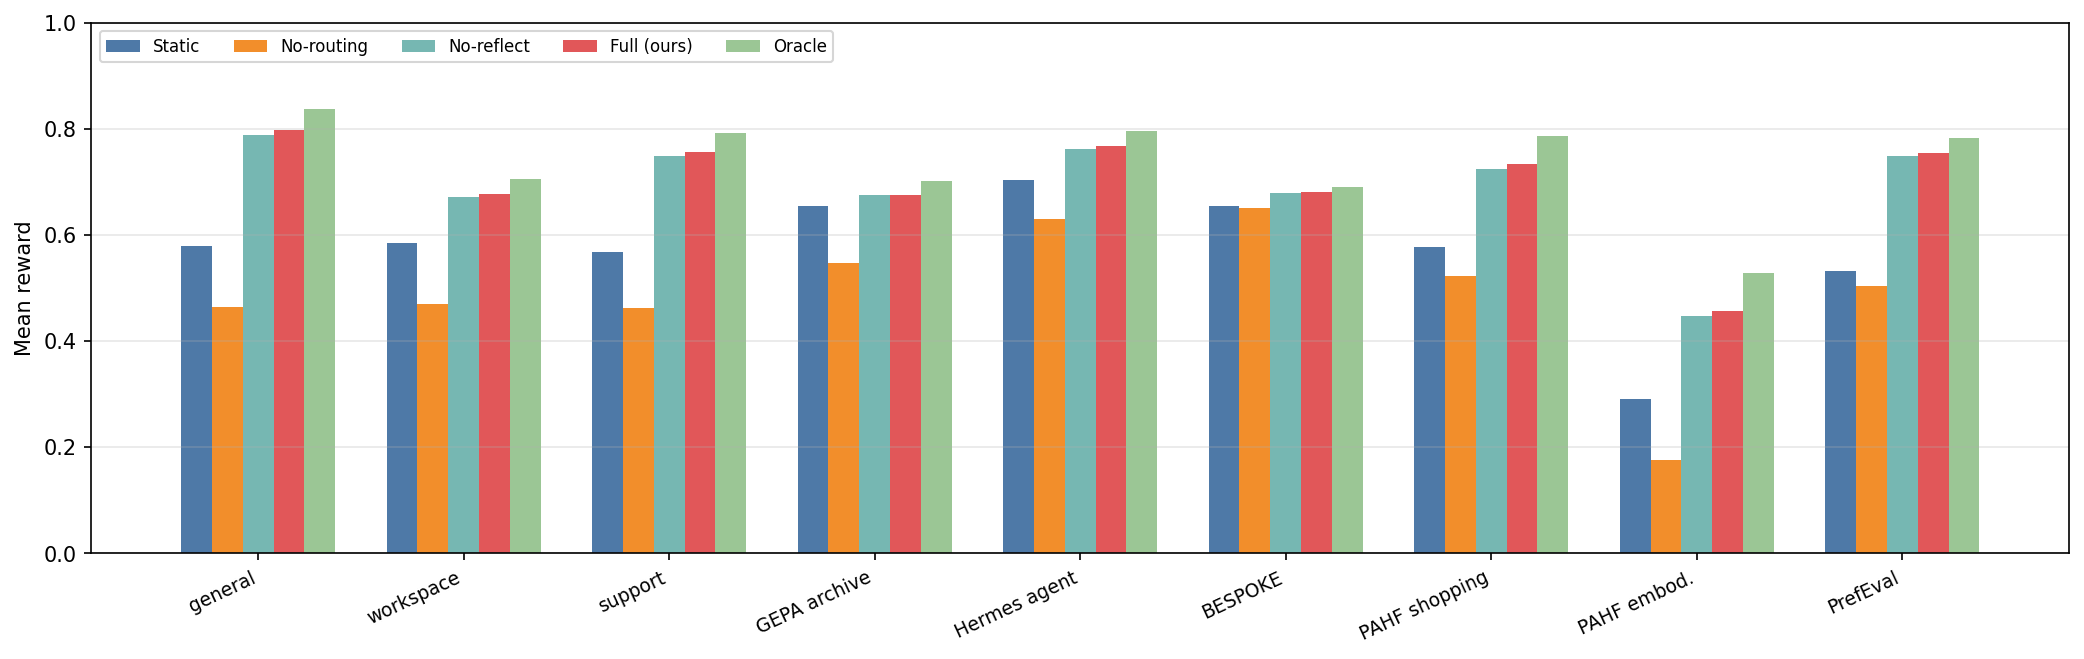
\includegraphics[width=\columnwidth]{fig_ablation_9benchmarks.png}
\caption{Mean reward for three router variants and two references on nine
benchmarks. Within each benchmark, the bars are ordered Static, No-routing,
No-reflect, Full, and Oracle from left to right. The bars show means without
uncertainty intervals.}
\label{fig:ablation}
\end{figure}

\paragraph{Per-round convergence.} Figure~\ref{fig:perround-matrix} shows
per-round reward traces for the same five series.

In all cases, PersonalEvo converges toward the oracle within ${\sim}50$ rounds, while the static baseline remains flat.

The figure plots reward rather than the observed-reward residual; per-seed
residuals appear in Tables~\ref{tab:app-regret} and
\ref{tab:app-regret-abl}. These finite traces do not identify an asymptotic
rate.

\begin{figure}[h]
\centering
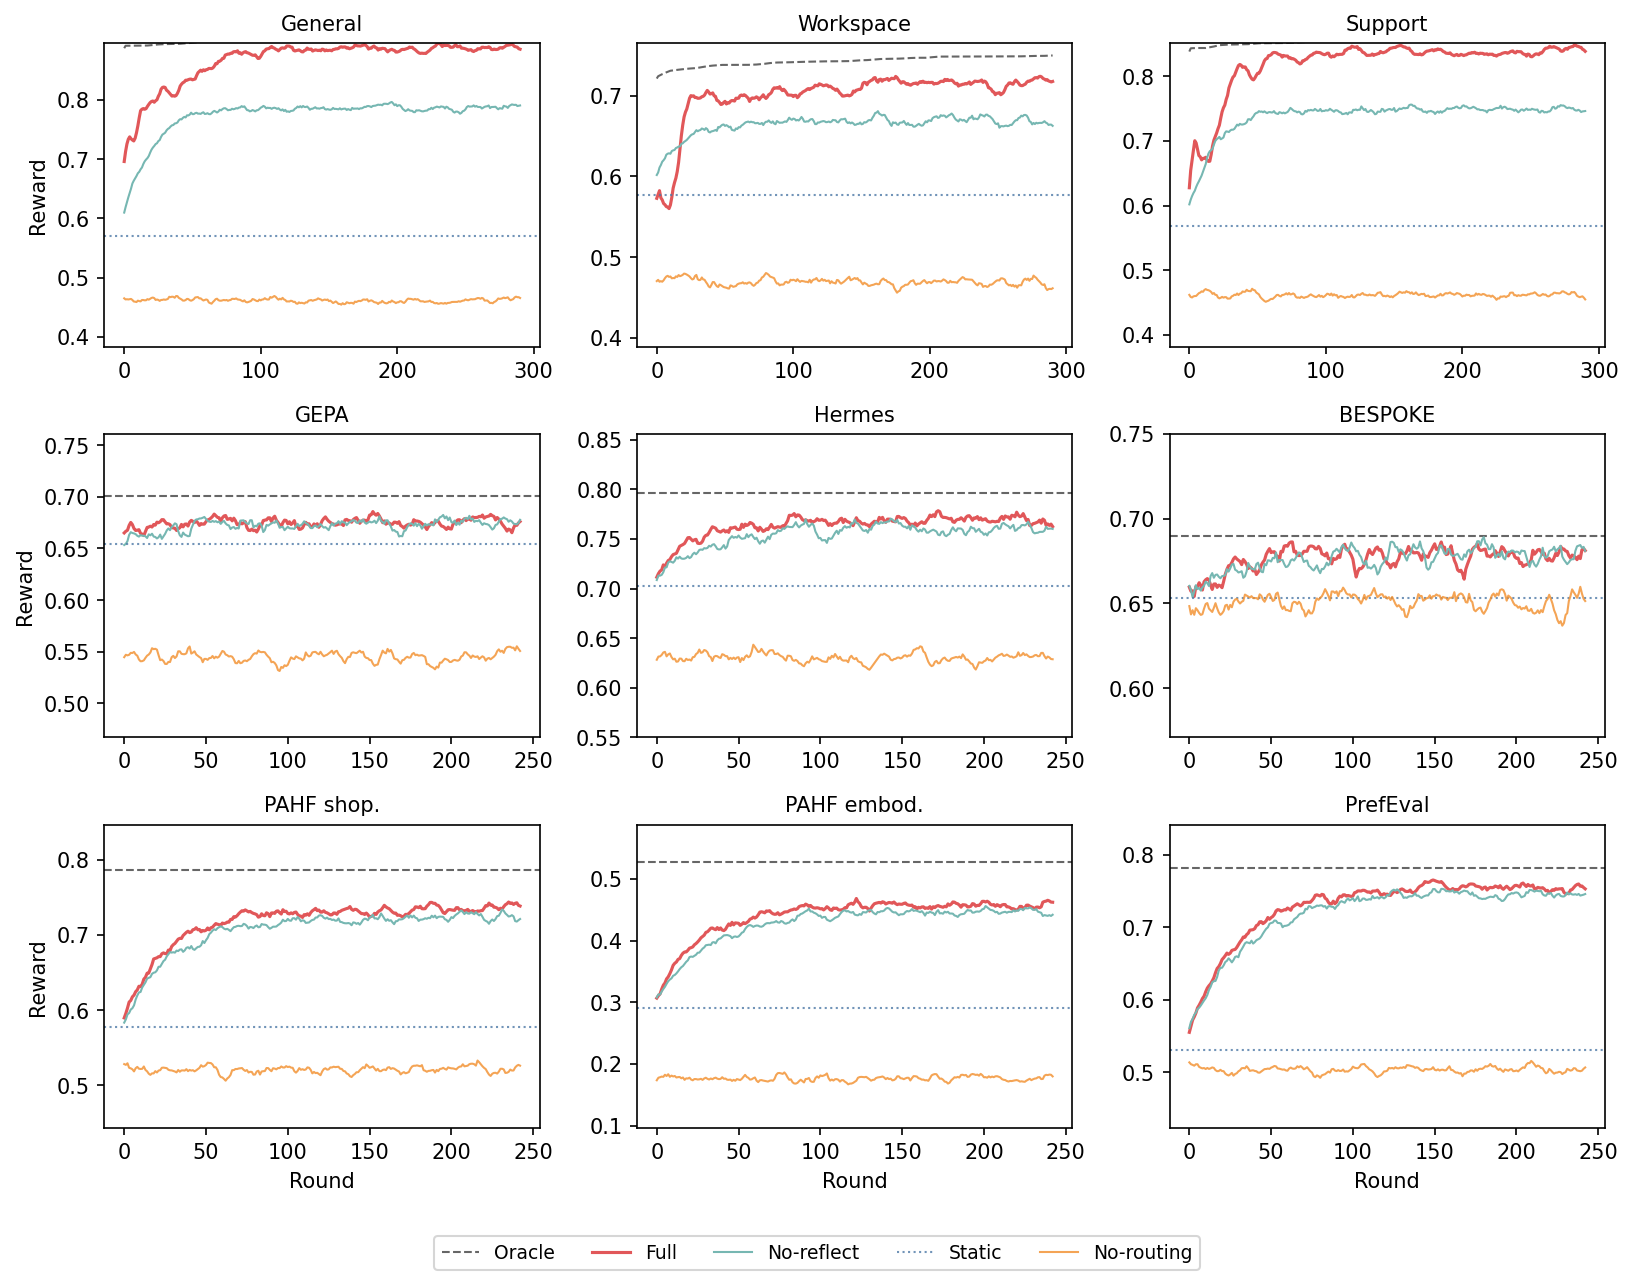
\includegraphics[width=\columnwidth]{fig_perround_3x3_matrix.png}
\caption{Per-round mean reward on nine benchmarks. The five series are
\textbf{Full} (red; concat features, gated reflection, LinUCB),
\textbf{No-reflect} (teal; frozen archive, $\bar G_T{=}0$),
\textbf{No-routing} (orange; uniform-random selection,
$\Delta_{\mathrm{route}}{\to}0$), \textbf{Static} (blue dotted; best single
candidate for all users), and \textbf{Oracle} (gray dashed; per-user optimum).
The curves show means without uncertainty bands, and the vertical range
differs by panel. The top row is synthetic; the remaining rows use framework
and real-data benchmarks.}
\label{fig:perround-matrix}
\end{figure}

\subsection{Comparison against existing routing methods}

\label{sec:exp-baselines}

To position PersonalEvo against prior routing strategies, we compare five methods on all nine benchmarks (Table~\ref{tab:baselines}): (i)~\textbf{Static}: deploy the single best-on-average candidate; (ii)~\textbf{GEPA-Pareto}: maintain the Pareto-optimal subset of the archive and deploy uniformly from it \citep{agrawal2025geparp}; (iii)~\textbf{Thompson}: Bayesian Thompson sampling over candidates \citep{pahf2025}; (iv)~\textbf{RouteLLM-thresh}: route users to specialist or generalist candidates based on a variance threshold; (v)~\textbf{PersonalEvo}: our full method.

\begin{table}[h]
\centering
\small
\resizebox{\columnwidth}{!}{
\begin{tabular}{lccccccc}
\toprule
\textbf{Benchmark} & \textbf{Static} & \textbf{GEPA-Pareto} & \textbf{Thompson} & \textbf{RouteLLM} & \textbf{PersonalEvo} & \textbf{Oracle} \\
\midrule
General            & $0.579$ & $0.533$ & $0.510$ & $0.732$ & $\mathbf{0.797}$ & $0.836$ \\
Workspace          & $0.585$ & $0.539$ & $0.515$ & $0.650$ & $\mathbf{0.678}$ & $0.705$ \\
Support            & $0.568$ & $0.525$ & $0.504$ & $0.700$ & $\mathbf{0.757}$ & $0.791$ \\
GEPA archive       & $0.671$ & $0.616$ & $0.569$ & $0.675$ & $\mathbf{0.681}$ & $0.701$ \\
Hermes agent       & $0.729$ & $0.644$ & $0.659$ & $0.750$ & $\mathbf{0.771}$ & $0.796$ \\
BESPOKE            & $0.681$ & $0.660$ & $0.654$ & $0.678$ & $\mathbf{0.682}$ & $0.690$ \\
PAHF shopping      & $0.625$ & $0.532$ & $0.560$ & $0.691$ & $\mathbf{0.754}$ & $0.812$ \\
PAHF embodied      & $0.290$ & $0.244$ & $0.222$ & $0.407$ & $\mathbf{0.457}$ & $0.528$ \\
PrefEval           & $0.531$ & $0.520$ & $0.514$ & $0.687$ & $\mathbf{0.754}$ & $0.782$ \\
\bottomrule
\end{tabular}
}
\caption{Comparison against existing routing methods on all nine benchmarks. Mean reward over 5 seeds. PersonalEvo (bold) achieves the highest reward among non-oracle methods in every row. GEPA-Pareto underperforms static because archive diversity without per-user routing is counterproductive. Thompson sampling explores too broadly. RouteLLM-threshold is the closest competitor but uses a fixed rule rather than learning per-user preferences.}
\label{tab:baselines}
\end{table}

The results reveal why the decomposition matters for method design: GEPA-Pareto maintains a diverse archive ($\bar G_T$ is high) but has no routing mechanism to exploit $\Delta_{\mathrm{route}}$, so diversity is wasted.

Thompson sampling routes but explores every arm equally regardless of user context, paying excessive $\bar L_T$.

RouteLLM routes by context but uses a fixed threshold rather than learning individual preferences.

PersonalEvo combines per-user routing with gated evolution and a small logged observed-reward residual. The experiment does not identify that residual with the theoretical \(\bar L_T\).

\subsection{Hyper-Ridge diagnostics and the remaining evaluation gap}
\label{sec:exp-hyper-ridge-plan}

The estimates in Table~\ref{tab:main}, ablations in
Figure~\ref{fig:ablation}, per-round traces in
Figure~\ref{fig:perround-matrix}, and baseline comparison in
Table~\ref{tab:baselines} all evaluate the \emph{base} PersonalEvo router. We
additionally ran a five-seed diagnostic suite for Hyper-Ridge PersonalEvo. We
keep it separate from the headline comparison because it covers seven rather
than nine adapters and does not log the mean-reward exploration cost as its
primary endpoint.

\paragraph{Known-geometry mechanism.}
We construct a diagnostic linear bandit in which $K=30$ candidate parameters are drawn from a planted rank-three covariance, contexts are dense random unit vectors, and the horizon is $T=400$. Table~\ref{tab:hyper-diagnostic} compares isotropic ridge, Hyper-Ridge given the true covariance, and Hyper-Ridge with the covariance periodically re-estimated from the candidate models, all with the same ridge weight $\lambda=0.5$. The true geometry cuts cumulative exploration cost by $46$--$59\%$, while the online estimate raises it by $7$--$19\%$. This diagnostic uses Gaussian parameters, unbounded linear rewards, and a fixed exploration multiplier, so it does not test the bounded-reward theorem or its rate. It only isolates the effect of supplying the correct geometry.

\begin{table}[H]
\centering
\small
\begin{tabular}{rrrrr}
\toprule
$d$ & Isotropic & Known $\Omega$ & Estimated $\Omega$ & Known-$\Omega$ reduction \\
\midrule
20  & 314.1 & 170.2 & 375.0 & $45.8\%$ \\
50  & 447.6 & 213.1 & 504.9 & $52.4\%$ \\
100 & 455.4 & 188.1 & 487.5 & $58.7\%$ \\
\bottomrule
\end{tabular}
\caption{Mean cumulative exploration cost over five seeds on planted rank-three problems ($K=30$, $T=400$, $\lambda=0.5$ for all three routers). Lower is better. This mechanism diagnostic does not satisfy the assumptions of Proposition~\ref{prop:deff-bound}.}
\label{tab:hyper-diagnostic}
\end{table}

\paragraph{Adapter diagnostic.}
With tuning seeds disjoint from the five reporting seeds, the periodic estimator improves mean reward over the isotropic router on six of seven adapters, with changes ranging from $+0.002$ on BESPOKE to $+0.048$ on Hermes, and loses $0.010$ on GEPA. These numbers are not evidence of cross-candidate geometry transfer. The adapter harness represents candidate $a$ by the one-hot vector $e_a$. Starting from $\widehat{\Omega}_1=I$, each candidate estimate then has support only on its own coordinate, so the covariance update remains diagonal. Accordingly, the full-covariance and diagonal-ridge variants match exactly on every adapter and seed. This ablation exposes a representation mismatch that a larger seed count cannot repair.

\paragraph{Remaining protocol.}
The complete comparison must run base, known-covariance, calibration-split
estimated-covariance, periodically estimated-covariance, and diagonal-ridge
routers on the same nine benchmarks, using a feature map with shared behavioral
directions. It must report all four mean-reward terms of
\eqref{eq:method-thesis}, with \(\widehat L_T^\mu\) as the primary endpoint
and \(\widehat L_T^{\mathrm{obs}}\) reported separately, as well as the fitted
regret exponent, covariance error, and
\(d_{\mathrm{eff}}(\widehat\Omega;X)\). Until that comparison is complete, we
do not claim an empirical advantage for the fully adaptive Hyper-Ridge router.

\paragraph{Implementation status.}
The repository implements both the base router and the periodic Hyper-Ridge estimator, together with an identity-reduction test showing that frozen $\widehat{\Omega}=I$ reproduces the base router's selections. The diagnostic results are stored in \texttt{results/hyper\_ridge/suite.json}; the missing component is the feature-aware, nine-benchmark evaluation above, not the router implementation itself.

\section{Conclusion}

\label{sec:conclusion}

This paper revised PersonalEvo around one idea: a self-evolving agent should
learn the geometry of its own archive. Theorem~\ref{thm:decomp} and
Corollary~\ref{cor:dominance} determine when personalized routing pays off.
Hyper-Ridge leaves the structural and discovery terms unchanged and targets
the exploration cost. It models candidate parameters with a shared geometry
\(\Omega\) and uses the effective dimension in \eqref{eq:hyper-deff}.
For known \(\Omega\), Proposition~\ref{prop:deff-bound} gives the complete
bound in \eqref{eq:hyper-deff-bound-expect-main}. For \(T\ge2\), fixed problem
parameters, and \(\delta=1/T\), both the LinUCB and known-geometry bounds are
\(O(\sqrt{T}\log T)\). Geometry helps only when the complete Hyper-Ridge budget
is smaller. The calibration-split theorem gives a separate frozen-estimate
bound whose explicit width-inflation and calibration remainder is
\(o(\sqrt T)\); it does not cover periodic re-estimation.

Two provenance facts bound what this paper claims. First, the nine-benchmark estimates, ablation hierarchy, per-round traces, and baseline comparison in Section~\ref{sec:experiments} belong to the \emph{base} LinUCB router. Their logged margins are
\begin{equation}
\label{eq:conc-margins}
\Delta_{\mathrm{route}}(A_1) + \bar G_T - \bar L_T^{\mathrm{obs}}
\;\in\; [+0.027,\, +0.295]
\end{equation}
across all nine benchmarks, where
\(\bar L_T^{\mathrm{obs}}=T^{-1}\sum_t(m_t-r_t)\). This equality is logged
accounting, not validation of \eqref{eq:thm-decomp-avg}: clipping means that
\(\mathbb E[r_t\mid\mathcal F_{t-1}]\) need not equal the pre-clipping
\(\mu(U,a_t)\) used by the structural terms. The selected-arm mean must be
logged to evaluate \(\bar L_T\) itself. The separate Hyper-Ridge suite is
diagnostic: known geometry helps on planted low-rank problems, but periodic
estimation does not recover that benefit, and one-hot adapters collapse the
full covariance to a diagonal one. Second, the effective-dimension guarantee
\eqref{eq:hyper-deff-bound-expect-main} is a theorem for the oracle-covariance router.
Appendix~\ref{app:err-control-proof} controls an estimated covariance for a
calibration-split procedure under explicit diversity conditions, but this
result does not cover the periodically updated estimator in
Algorithm~\ref{alg:hyper-ridge}. Controlling that fully adaptive estimator
remains the primary theoretical open problem.

The corresponding empirical open problem is the complete comparison specified in Section~\ref{sec:exp-hyper-ridge-plan}: base LinUCB versus known-covariance, calibration-split, periodically estimated, and diagonal-ridge routers on the same nine benchmarks, with the mean-reward exploration cost $\widehat L_T^\mu$ as the primary endpoint and $\widehat L_T^{\mathrm{obs}}$ reported separately. The feature map must admit shared directions; otherwise the full model is diagonal by construction. The comparison should also report covariance error, the fitted regret exponent, and a per-benchmark estimate of $d_{\mathrm{eff}}(\widehat\Omega;X)$ to locate both sides of the boundary: regimes where
$d_{\mathrm{eff}}(\Omega;X)\ll d$ and the geometric potential can be smaller,
and near-isotropic regimes where $d_{\mathrm{eff}}(\Omega;X)\approx d$. In both cases, the full confidence
budget determines the comparison. The current implementation supplies the
periodic estimator and common harness; a calibration-split implementation and
a shared feature representation remain to be added.

Beyond the two named gaps, the limitations of the base framework carry over. The reflective proposer in the simulated environments is oracle-assisted, so the measured evolution gain $\bar G_T$ does not estimate what a realistic LLM-driven proposer would deliver, and each user maintains a private archive, so discoveries are not shared across users. A shared archive could provide more data for estimating \(\Omega\), but it would change the predictability argument in Lemma~\ref{lem:predictable}; we leave that setting open. The decomposition \eqref{eq:thm-decomp-avg} also applies to model routing, prompt selection, and tool-use policies whenever a system must choose from a candidate library.

\appendix

\section{Appendix Proofs: Preliminaries and the Exact Decomposition}

\label{app:proofs}

This appendix block fixes the probability model used by all proofs and proves the first main theorem: the exact four-term decomposition.

The proof is an accounting identity; it does not use a contextual-bandit regret theorem and does not assume that reflection is realistic.

\subsection{Probability space and online objects}

All random variables are defined on a common probability space
\((\Xi,\mathcal F,\mathbb P)\), and expectations average over both the
population draw and the online trajectory.  The evaluation user is
\(U\sim\Pi\) with values in \(\mathcal U\), and candidates belong to
\(\mathcal A\).  The common initial archive is \(A_1\subseteq\mathcal A\);
before round \(t\), the current archive is \(A_t(U)\subseteq\mathcal A\), and
the router selects \(a_t(U)\in A_t(U)\).  Mean and observed rewards satisfy
\begin{equation}
\mu:\mathcal U\times\mathcal A\to[0,1],
\qquad
r_t=\mu(U,a_t(U))+\xi_t.
\end{equation}
For the later plug-in bounds, let
\(\mathcal F_0\subseteq\cdots\subseteq\mathcal F_T\) be the online filtration
and \(x_t(a)\in\mathbb R^d\) the feature vector for candidate \(a\).  The exact
decomposition uses only bounded rewards and the archive conditions; the noise
and feature assumptions are recorded for the later results.

\begin{assumption}[A1: bounded mean reward]
\label{ass:app-bounded}
For every user \(u\) and candidate \(a\),
\(0\leq\mu(u,a)\leq 1\).
\end{assumption}

\begin{assumption}[A2: finite common initial archive]
\label{ass:app-finite-initial}
The initial archive is deterministic, nonempty, and finite:
\(1\leq |A_1|<\infty\).
\end{assumption}

\begin{assumption}[A3: finite append-only online archives]
\label{ass:app-append-only}
For every round, \(1\leq |A_t(U)|<\infty\) almost surely, and the archive is
append-only: \(A_t(U)\subseteq A_{t+1}(U)\).
\end{assumption}

\begin{assumption}[A4: predictable archive]
\label{ass:app-predictable}
Before the router chooses at round \(t\), the archive is measurable with
respect to the past: \(\sigma(A_t(U))\subseteq\mathcal F_{t-1}\).
\end{assumption}

\begin{assumption}[A5: centered conditionally sub-Gaussian noise]
\label{ass:app-noise}
For every \(\lambda\in\mathbb R\),
\begin{equation}
\begin{aligned}
\mathbb E[\xi_t\mid\mathcal F_{t-1}] &\,=\,0, &
\mathbb E\!\left[e^{\lambda\xi_t}\mid\mathcal F_{t-1}\right]
&\,\leq\,\exp\!\left(\frac{\lambda^2\sigma^2}{2}\right).
\end{aligned}
\end{equation}
\end{assumption}

\begin{assumption}[A6: bounded features]
\label{ass:app-features}
Every available candidate satisfies \(\|x_t(a)\|_2\leq L\).
\end{assumption}

\subsection{Values and accounting terms}

For a deterministic finite archive \(A\), define its static value, routed
value, and heterogeneity gain by
\begin{equation}
\begin{aligned}
V_{\mathrm{static}}(A)
&\,=\,\max_{a\in A}\mathbb E[\mu(U,a)], &
V_{\mathrm{route}}(A)
&\,=\,\mathbb E\!\left[\max_{a\in A}\mu(U,a)\right], \\
\Delta_{\mathrm{route}}(A)
&\,=\,V_{\mathrm{route}}(A)-V_{\mathrm{static}}(A).
\end{aligned}
\end{equation}
For the online archive, define
\begin{equation}
\begin{aligned}
m_t(U)
&\,=\,\max_{a\in A_t(U)}\mu(U,a), &
G_t(U)
&\,=\,m_t(U)-m_1(U), &
L_t(U)
&\,=\,m_t(U)-\mu(U,a_t(U)), \\
\bar G_T
&\,=\,\frac1T\sum_{t=1}^T\mathbb E[G_t(U)], &
\bar L_T
&\,=\,\frac1T\sum_{t=1}^T\mathbb E[L_t(U)].
\end{aligned}
\end{equation}

\begin{proposition}[Integrability and signs of the accounting terms]
\label{prop:1}
Under Assumptions~\ref{ass:app-bounded}--\ref{ass:app-append-only}, the current-archive optimum satisfies
\begin{equation}
m_t(U),G_t(U),L_t(U)\in[0,1],
\qquad
\mathbb E|m_t(U)|+\mathbb E|G_t(U)|+\mathbb E|L_t(U)|
\,\leq\,3.
\end{equation}
\end{proposition}

\begin{proof}
Bounded rewards give \(0\leq m_t(U)\leq1\).  Since
\(a_t(U)\in A_t(U)\), and since append-only growth gives
\(A_1\subseteq A_t(U)\),
\begin{equation}
\begin{aligned}
0
&\,\leq\,m_t(U)-\mu(U,a_t(U))
      \,=\,L_t(U)\,\leq\,1, \\
0
&\,\leq\,m_t(U)-m_1(U)
      \,=\,G_t(U)\,\leq\,1.
\end{aligned}
\end{equation}
The integrability bound follows by summing these three pointwise bounds.
\end{proof}

\subsection{Supporting lemmas for the four-term decomposition}

\begin{lemma}[Static-versus-routed value]
\label{lem:1}
For every deterministic, finite, nonempty archive \(A\),
\(\Delta_{\mathrm{route}}(A)\geq0\).  Equality holds if and only if some
\(a^\star\in A\) is pointwise optimal almost surely:
\begin{equation}
\mu(U,a^\star)
\,=\,
\max_{a\in A}\mu(U,a)
\quad
\text{almost surely}.
\end{equation}
In particular, the inequality is strict if every candidate is suboptimal with
positive probability:
\begin{equation}
\forall a\in A,
\qquad
\mathbb{P}\!\left(
\mu(U,a)
<
\max_{b\in A}\mu(U,b)
\right)
>
0.
\end{equation}
\end{lemma}

\begin{proof}
Because \(A\) is finite, choose
\(a^\star\in\operatorname*{arg\,max}_{a\in A}
\mathbb E[\mu(U,a)]\).  Pointwise maximality gives
\begin{equation}
\begin{aligned}
\Delta_{\mathrm{route}}(A)
&\,=\,\mathbb E\!\left[
  \max_{a\in A}\mu(U,a)-\mu(U,a^\star)\right]
\,\geq\,0.
\end{aligned}
\end{equation}
The integrand is nonnegative, so its expectation is zero exactly when it is
zero almost surely.  This proves the equality condition.  Conversely, an
almost-surely pointwise-optimal candidate attains both
\(V_{\mathrm{static}}(A)\) and \(V_{\mathrm{route}}(A)\).  Under the stated
strictness condition, the integrand is positive with positive probability for
every possible static maximizer, so its expectation is positive.
\end{proof}

\begin{lemma}[Pointwise routed-value accounting]
\label{lem:2}
For every round \(t\), the preceding definitions imply
\begin{equation}
\mu(U,a_t(U))
\,=\,
m_1(U)+G_t(U)-L_t(U).
\end{equation}
\end{lemma}

\begin{proof}
Rearrange \(L_t(U)=m_t(U)-\mu(U,a_t(U))\) and substitute
\(m_t(U)=m_1(U)+G_t(U)\).
\end{proof}

\subsection{First main theorem: four-term decomposition}

\begin{theorem}[Exact decomposition over the common initial archive]
\label{thm:main}
This restates Theorem~\ref{thm:decomp}.  Let \(U\sim\Pi\), let
\(1\leq |A_1|<\infty\), and suppose \(a_t(U)\in A_t(U)\).  Then, for every
round \(t\),
\begin{equation}
\mathbb{E}[\mu(U,a_t(U))]
\,=\,
V_{\mathrm{static}}(A_1)
+
\Delta_{\mathrm{route}}(A_1)
+
\mathbb{E}[G_t(U)]
-
\mathbb{E}[L_t(U)].
\end{equation}
Define
\begin{equation}
\begin{aligned}
R_T
&\,=\,\frac1T\sum_{t=1}^T\mathbb E[\mu(U,a_t(U))], &
\bar G_T
&\,=\,\frac1T\sum_{t=1}^T\mathbb E[G_t(U)], &
\bar L_T
&\,=\,\frac1T\sum_{t=1}^T\mathbb E[L_t(U)].
\end{aligned}
\end{equation}
Then
\begin{equation}
\label{eq:app-decomp-bound}
R_T
\,=\,
V_{\mathrm{static}}(A_1)
+
\Delta_{\mathrm{route}}(A_1)
+
\bar G_T
-
\bar L_T.
\end{equation}
\end{theorem}

\begin{proof}
Proposition~\ref{prop:1} ensures integrability.  Taking expectations in
Lemma~\ref{lem:2} gives
\begin{equation}
\begin{aligned}
\mathbb{E}[\mu(U,a_t(U))]
&\,=\,
  \mathbb E[m_1(U)]+\mathbb E[G_t(U)]-\mathbb E[L_t(U)] \\
&\,=\,
  V_{\mathrm{route}}(A_1)+\mathbb E[G_t(U)]-\mathbb E[L_t(U)] \\
&\,=\,
V_{\mathrm{static}}(A_1)
+
\Delta_{\mathrm{route}}(A_1)
+
\mathbb E[G_t(U)]
-
\mathbb E[L_t(U)].
\end{aligned}
\end{equation}
Summing over \(t\) and dividing by \(T\) proves
\eqref{eq:app-decomp-bound}.
\end{proof}

The theorem concerns mean rewards.  Under Assumption~\ref{ass:app-noise}, the
same expectation governs unclipped observed rewards because
\begin{equation}
\label{eq:app-observed-mean-link}
\begin{aligned}
\mathbb{E}[r_t]
&\,=\,\mathbb E[\mu(U,a_t(U))]+\mathbb E[\xi_t] \\
&\,=\,
\mathbb{E}[\mu(U,a_t(U))].
\end{aligned}
\end{equation}

This link does not apply to the saved simulator's clipped observations in
\eqref{eq:exp-clipped-reward} when \(\mu\) denotes the pre-clipping mean.
The following \texttt{general} row instead checks the separate observed-reward
accounting identity.  Its measured terms are
\begin{equation}
V_{\mathrm{static}}(A_1)=0.570,\quad
\Delta_{\mathrm{route}}(A_1)=0.280,\quad
\bar G_T=0.051,\quad
\bar L_T^{\mathrm{obs}}=0.036.
\end{equation}
Therefore,
\begin{equation}
\label{eq:app-numeric-closure}
\begin{aligned}
V_{\mathrm{static}}(A_1)
+
\Delta_{\mathrm{route}}(A_1)
+
\bar G_T
-
\bar L_T^{\mathrm{obs}}
&\,=\,
0.570+0.280+0.051-0.036
\\
&\,=\,
0.865,
\end{aligned}
\end{equation}

which matches the reported observed routed value \(0.864\) up to table
rounding. Because \(\bar L_T^{\mathrm{obs}}\) is defined from the same routed
rewards, this is an algebraic consistency check rather than empirical
validation of Theorem~\ref{thm:main}.

\section{Appendix Proofs: Second Main Theorem and Intermediate Lemmas}

\label{app:proofs2}

This section proves the second main theorem, the conditional plug-in statement for the exploration cost.

The proof does not assert a new regret rate; it shows how any valid bound on the cumulative exploration cost plugs into the four-term decomposition of Theorem~\ref{thm:main}.

\begin{assumption}[External expected exploration-cost bound]
\label{ass:app-external-tax}
For \(T\in\mathbb N\), there is a deterministic \(B_T\geq0\) such that
\begin{equation}
\label{eq:app-external-tax-assumption}
\sum_{t=1}^{T}\mathbb{E}[L_t(U)]
\,\leq\,
B_T.
\end{equation}
\end{assumption}

The next lemma records the conditioning fact that makes growing archives compatible with standard martingale arguments, provided children are appended only after the current reward is observed.

\begin{lemma}[Predictable archive conditioning]
\label{lem:3}
Let the pre-action sigma-field be
\begin{equation}
\mathcal{H}_{t-1}
\,=\,
\sigma\!\left(
U,\,
A_1,\,
\{a_s(U),r_s,A_{s+1}(U):1\,\le\, s<t\}
\right).
\end{equation}
Assume \(A_t(U)\) is \(\mathcal H_{t-1}\)-measurable and at most \(K_{\max}\)
candidates appear by time \(T\).  Index them by deterministic birth-order
slots \(k\leq K_{\max}\), with stopping-time birth \(\tau_k\) and
\(\tau_k=\infty\) for an unfilled slot.  On \(\{\tau_k\leq T\}\), the identity
\(a^{(k)}\) and its feature rule are
\(\mathcal H_{\tau_k-1}\)-measurable.  Define the padded feature and selection
indicator
\begin{equation}
\begin{aligned}
\widetilde x_{t,k}
&\,=\,\mathbf 1\{\tau_k\leq t\}\psi(U,a^{(k)}), &
I_{t,k}
&\,=\,\mathbf 1\{\tau_k\leq t,\ a_t(U)=a^{(k)}\}.
\end{aligned}
\end{equation}
Assume both are \(\mathcal H_{t-1}\)-measurable: they are zero before birth,
and the slot identity is in the pre-action history afterward.  Also assume
\begin{equation}
\begin{aligned}
\mathbb E[\xi_t\mid\mathcal H_{t-1}]
&\,=\,0, &
\mathbb{E}\!\left[\exp(s\xi_t)\mid \mathcal{H}_{t-1}\right]
&\,\leq\,
\exp\!\left(\frac{s^2\sigma^2}{2}\right)
\quad\text{for all }s\in\mathbb R.
\end{aligned}
\end{equation}
Then, for each deterministic slot \(k\),
\begin{equation}
Z_{t,k}=I_{t,k}\widetilde x_{t,k}\xi_t,
\qquad
M_{n,k}=\sum_{t=1}^n Z_{t,k}
\end{equation}
defines a vector-valued martingale with respect to the post-round filtration.
\end{lemma}

\begin{proof}
Fix \(k\).  Since \(I_{t,k}\widetilde x_{t,k}\) is
\(\mathcal H_{t-1}\)-measurable,
\begin{equation}
\begin{aligned}
\mathbb{E}[Z_{t,k}\mid \mathcal{H}_{t-1}]
&\,=\,
I_{t,k}\widetilde x_{t,k}\,
\mathbb{E}[\xi_t\mid \mathcal{H}_{t-1}]
\,=\,0.
\end{aligned}
\end{equation}
Moreover, for any direction \(v\),
\begin{equation}
\begin{aligned}
\mathbb{E}\!\left[
\exp\!\left(s\,v^\top Z_{t,k}\right)
\mid
\mathcal{H}_{t-1}
\right]
&\,\le\,
\exp\!\left(
\frac{s^2\sigma^2}{2}
I_{t,k}
(v^\top\widetilde x_{t,k})^2
\right).
\end{aligned}
\end{equation}
Thus the increments are conditionally mean-zero (and sub-Gaussian in every
predictable direction), so their partial sums form the claimed martingale.
\end{proof}

The following elementary conversion is useful because many router analyses produce high-probability regret bounds, whereas Theorem~\ref{thm:main} is stated in expectation.

\begin{lemma}[From high-probability tax to expected tax]
\label{lem:4}
Suppose \(0\leq\mu(U,a)\leq1\), let
\(S_T^L=\sum_{t=1}^T L_t(U)\), and let
\(\widetilde B_T\geq0\) and \(\delta\in(0,1)\) satisfy
\begin{equation}
\mathbb{P}\!\left(S_T^{L}\leq \widetilde{B}_T\right)
\,\geq\,
1-\delta.
\end{equation}
Then
\begin{equation}
\sum_{t=1}^{T}\mathbb{E}[L_t(U)]
\,\leq\,
\widetilde{B}_T+T\delta.
\end{equation}
\end{lemma}

\begin{proof}
Because \(a_t(U)\in A_t(U)\) and rewards lie in \([0,1]\),
\(0\leq L_t(U)\leq1\), hence \(0\leq S_T^L\leq T\).  For
\(\mathcal E_T^L=\{S_T^L\leq\widetilde B_T\}\),
\begin{equation}
\begin{aligned}
\mathbb{E}[S_T^{L}]
&\,=\,
\mathbb{E}[S_T^{L}\mathbf{1}\{\mathcal{E}_T^{L}\}]
+
\mathbb{E}[S_T^{L}\mathbf{1}\{(\mathcal{E}_T^{L})^c\}]
\\
&\,\le\,
\widetilde{B}_T
+
T\,\mathbb{P}((\mathcal{E}_T^{L})^c)
\\
&\,\le\,
\widetilde{B}_T
+
T\delta.
\end{aligned}
\end{equation}
Linearity of expectation completes the proof.
\end{proof}

We next give one sufficient route to Assumption~\ref{ass:app-external-tax}.

This proposition is not a new contribution of the paper; it is a standard disjoint-linear UCB certificate written only to clarify what must be true for the plug-in theorem to inherit a familiar rate.

\begin{proposition}[Disjoint-linear certificate for the external tax bound]
\label{prop:2}
Let \(d\in\mathbb N\) and
\(\mathcal A_T(U)=\bigcup_{t=1}^T A_t(U)\), with
\(|\mathcal A_T(U)|\leq K_{\max}\).  Use the deterministic birth-order slots
from Lemma~\ref{lem:3}.  Let \((\mathcal G_t)\) be an analysis filtration with
\(\mathcal H_t\subseteq\mathcal G_t\).  Each \(\tau_k\) is an
\(\mathcal H_t\)-stopping time; the candidate identity and feature rule are
\(\mathcal H_{\tau_k-1}\)-measurable, while its latent parameter is fixed at
birth and \(\mathcal G_{\tau_k-1}\)-measurable.  The zero-padded process is
\(\mathcal G_t\)-predictable.  The router remains \(\mathcal H_t\)-adapted and
does not observe the latent parameter.

For every realized candidate \(a\), suppose
\begin{equation}
x_t(a)=\psi(U,a)\in\mathbb R^d,\qquad
\|x_t(a)\|_2\leq L_x,\qquad
\|\theta_a^\star\|_2\leq S,\qquad
\mu(U,a)=x_t(a)^\top\theta_a^\star.
\end{equation}
Let \(r_t=\mu(U,a_t(U))+\xi_t\), where the centered sub-Gaussian conditions of
Lemma~\ref{lem:3} also hold conditionally on \(\mathcal G_{t-1}\).  For
\(\lambda\geq L_x^2>0\), define
\begin{equation}
\begin{aligned}
V_{t,a}
&\,=\,
\lambda I_d
+
\sum_{s=1}^{t-1}
\mathbf{1}\{a_s(U)=a\}\,x_s(a)x_s(a)^\top, \\
\widehat{\theta}_{t,a}
&\,=\,
V_{t,a}^{-1}
\sum_{s=1}^{t-1}
\mathbf{1}\{a_s(U)=a\}\,x_s(a)r_s.
\end{aligned}
\end{equation}
For \(\delta\in(0,1)\), let
\begin{equation}
\beta_T(\delta)
\,=\,
\sigma
\sqrt{
2\log\!\left(\frac{K_{\max}}{\delta}\right)
+
d\log\!\left(1+\frac{T L_x^2}{\lambda d}\right)
}
+
\sqrt{\lambda}\,S.
\end{equation}
If the router uses the disjoint UCB rule
\begin{equation}
a_t(U)
\,\in\,
\operatorname*{arg\,max}_{a\in A_t(U)}
\left\{
x_t(a)^\top\widehat{\theta}_{t,a}
+
\beta_T(\delta)
\sqrt{x_t(a)^\top V_{t,a}^{-1}x_t(a)}
\right\}
\end{equation}
then, with probability at least \(1-\delta\),
\begin{equation}
\sum_{t=1}^{T}L_t(U)
\,\leq\,
B_T^{\mathrm{lin}}(\delta),
\end{equation}
where
\begin{equation}
B_T^{\mathrm{lin}}(\delta)
\,=\,
2\beta_T(\delta)
\sqrt{
2T K_{\max} d
\log\!\left(1+\frac{T L_x^2}{\lambda d}\right)
}.
\end{equation}
Consequently,
\begin{equation}
\sum_{t=1}^{T}\mathbb{E}[L_t(U)]
\,\leq\,
B_T^{\mathrm{lin}}(\delta)+T\delta.
\end{equation}
\end{proposition}

\begin{proof}
Write \(a_t=a_t(U)\).  For each deterministic slot \(k\), let
\begin{equation}
M_{t,k}
\,=\,
\sum_{s=1}^{t-1}
\mathbf{1}\{a_s=a^{(k)}\}\,x_s(a^{(k)})\xi_s,
\end{equation}
with zero summands before \(\tau_k\).  Conditional on the slot's birth history,
the noise and measurability assumptions make this a vector-valued martingale
in the analysis filtration.  The
self-normalized martingale inequality gives
\begin{equation}
\begin{aligned}
\mathbb{P}\!\left(
\exists t\leq T:
\|M_{t,k}\|_{V_{t,a^{(k)}}^{-1}}
>
\sigma
\sqrt{
2\log\!\left(\frac{K_{\max}}{\delta}\right)
+
\log\!\left(\frac{\det V_{t,a^{(k)}}}{\det(\lambda I_d)}\right)
}
\right)
&\,\leq\,
\frac{\delta}{K_{\max}}.
\end{aligned}
\end{equation}
The trace bound gives, uniformly in \(t\leq T\),
\begin{equation}
\begin{aligned}
\log\!\left(\frac{\det V_{t,a^{(k)}}}{\det(\lambda I_d)}\right)
&\,\leq\,
d\log\!\left(
1+
\frac{1}{\lambda d}
\sum_{s=1}^{t-1}
\mathbf{1}\{a_s=a^{(k)}\}\|x_s(a^{(k)})\|_2^2
\right)
\\
&\,\leq\,
d\log\!\left(
1+\frac{T L_x^2}{\lambda d}
\right).
\end{aligned}
\end{equation}
Union-bounding over the deterministic slots yields, with probability at least
\(1-\delta\),
\begin{equation}
\forall t\,\le\, T,\,
\forall a\in A_t(U):
\left|
x_t(a)^\top(\widehat{\theta}_{t,a}-\theta_a^\star)
\right|
\,\leq\,
\beta_T(\delta)
\sqrt{x_t(a)^\top V_{t,a}^{-1}x_t(a)}.
\end{equation}
On this event, write
\(\widehat\mu_t(a)=x_t(a)^\top\widehat\theta_{t,a}\),
\(z_t(a)=\sqrt{x_t(a)^\top V_{t,a}^{-1}x_t(a)}\), and choose
\begin{equation}
a_t^\star
\,\in\,
\operatorname*{arg\,max}_{a\in A_t(U)}\mu(U,a).
\end{equation}
Confidence, the UCB choice, and confidence again give
\begin{equation}
\begin{aligned}
\mu(U,a_t^\star)
&\,\leq\,
\widehat{\mu}_t(a_t^\star)
+
\beta_T(\delta)z_t(a_t^\star)
\\
&\,\leq\,
\widehat{\mu}_t(a_t)
+
\beta_T(\delta)z_t(a_t)
\\
&\,\leq\,
\mu(U,a_t)
+
2\beta_T(\delta)z_t(a_t).
\end{aligned}
\end{equation}
Thus \(L_t(U)\leq2\beta_T(\delta)z_t(a_t)\).  Also
\(z_t(a_t)^2\leq\|x_t(a_t)\|_2^2/\lambda\leq1\).  The determinant recursion
for each arm and a sum over at most \(K_{\max}\) arms give
\begin{equation}
\begin{aligned}
\sum_{t=1}^{T}
\mathbf{1}\{a_t=a\}z_t(a)^2
&\,\leq\,
2
\log\!\left(
\frac{\det V_{T+1,a}}{\det(\lambda I_d)}
\right)
\,\leq\,
2d
\log\!\left(1+\frac{T L_x^2}{\lambda d}\right), \\
\sum_{t=1}^{T}z_t(a_t)^2
&\,\leq\,
2K_{\max}d
\log\!\left(1+\frac{T L_x^2}{\lambda d}\right).
\end{aligned}
\end{equation}
Combining this with Cauchy--Schwarz yields
\begin{equation}
\begin{aligned}
\sum_{t=1}^{T}L_t(U)
&\,\leq\,
2\beta_T(\delta)
\sum_{t=1}^{T}z_t(a_t)
\\
&\,\leq\,
2\beta_T(\delta)
\sqrt{
2T K_{\max}d
\log\!\left(1+\frac{T L_x^2}{\lambda d}\right)
}
\\
&\,=\,
B_T^{\mathrm{lin}}(\delta).
\end{aligned}
\end{equation}
Lemma~\ref{lem:4} gives the expected bound.
\end{proof}

\begin{theorem}[Conditional plug-in regret for PersonalEvo]
\label{thm:convergence}
Use \(R_T\), \(\bar G_T\), and \(\bar L_T\) from
Theorem~\ref{thm:main}.  If
\begin{equation}
\label{eq:app-plugin-tax-assumption}
\sum_{t=1}^{T}\mathbb{E}[L_t(U)]
\,\leq\,
B_T
\end{equation}
then
\begin{equation}
R_T
\,\geq\,
V_{\mathrm{static}}(A_1)
+
\Delta_{\mathrm{route}}(A_1)
+
\bar G_T
-
\frac{B_T}{T}.
\end{equation}
\end{theorem}

\begin{proof}
The assumption gives \(\bar L_T\leq B_T/T\).  Substitute this into the exact
decomposition in Theorem~\ref{thm:main}.
\end{proof}

\begin{corollary}[Plug-in dominance condition]
\label{cor:app-plugin-dominance}
Under Theorem~\ref{thm:convergence}, personalized routing beats the best
static initial candidate whenever
\begin{equation}
\Delta_{\mathrm{route}}(A_1)
+
\bar G_T
>
\frac{B_T}{T}.
\end{equation}
In that case, \(R_T>V_{\mathrm{static}}(A_1)\).  On a fixed archive, where
\(\bar G_T=0\), the condition becomes
\begin{equation}
\Delta_{\mathrm{route}}(A_1)
>
\frac{B_T}{T}.
\end{equation}
\end{corollary}

\begin{proof}
Subtract \(V_{\mathrm{static}}(A_1)\) from the bound in
Theorem~\ref{thm:convergence}.  The stated condition makes the remaining
right-hand side positive.
\end{proof}

\begin{corollary}[Disjoint-LinUCB plug-in instance]
\label{cor:app-linucb-plugin}
If the conditions of Proposition~\ref{prop:2} hold, then
\begin{equation}
R_T
\,\geq\,
V_{\mathrm{static}}(A_1)
+
\Delta_{\mathrm{route}}(A_1)
+
\bar G_T
-
\frac{B_T^{\mathrm{lin}}(\delta)+T\delta}{T}.
\end{equation}
For \(\delta=1/T\), and with \(K_{\max}\), \(d\), \(L_x\), \(\lambda\), \(S\),
and \(\sigma\) fixed, the tax term satisfies
\begin{equation}
\frac{B_T^{\mathrm{lin}}(1/T)+1}{T}
\,=\,
O\!\left(\frac{\log T}{\sqrt T}\right)
\end{equation}
\end{corollary}

\begin{proof}
Apply Theorem~\ref{thm:convergence} with
\(B_T=B_T^{\mathrm{lin}}(\delta)+T\delta\).  For \(T\geq2\) and
\(\delta=1/T\), the definition of \(B_T^{\mathrm{lin}}\) gives
\begin{equation}
\begin{aligned}
\frac{B_T^{\mathrm{lin}}(1/T)+1}{T}
&\,=\,
\frac{
2\beta_T(1/T)
\sqrt{
2T K_{\max}d
\log\!\left(1+\frac{T L_x^2}{\lambda d}\right)
}
+1
}{T}
\\
&\,=\,
O\!\left(\frac{\log T}{\sqrt T}\right),
\end{aligned}
\end{equation}
under fixed problem parameters.
\end{proof}

As a scale check, suppose a valid certificate on the \texttt{workspace}
environment gave \(B_T/T=0.050\).  Table~\ref{tab:main} reports
\(V_{\mathrm{static}}(A_1)=0.577\),
\(\Delta_{\mathrm{route}}(A_1)=0.124\), and \(\bar G_T=0.041\).  The plug-in
bound would then be
\begin{equation}
\begin{aligned}
V_{\mathrm{static}}(A_1)
+
\Delta_{\mathrm{route}}(A_1)
+
\bar G_T
-
\frac{B_T}{T}
&\,=\,
0.577+0.124+0.041-0.050
\\
&\,=\,
0.692.
\end{aligned}
\end{equation}
This exceeds the static comparator by \(0.115\).  The empirical exploration
cost in Section~\ref{sec:experiments} is diagnostic, not a certificate; using
it only as a scale check gives
\(0.577+0.124+0.041-0.043=0.699\), which matches the reported routed value up
to rounding.  Proposition~\ref{prop:2} states the additional conditions needed
to replace that diagnostic curve by a certified \(B_T\).

\section{Proof of the Third Main Theorem and Complexity Consequences}

\label{app:proofs3}

This proof block concerns the narrowed third theorem from Section~\ref{sec:theory}.

The theorem is not a contraction theorem for language-model reflection; it is a conditional stopping-time statement for the first useful child under an explicit repair-probability assumption.

\begin{assumption}[Conditional repair probability for an active cluster]
\label{assump:app-repair}
Let \(\mathcal G=\{1,\ldots,K_{\mathrm{cl}}\}\), let \(g(U)\in\mathcal G\)
denote the user's cluster, and assume every cluster considered below has
positive mass
\begin{equation}
\pi_g
\,\coloneqq\,
\mathbb P(g(U)=g)
\,>\,
0.
\end{equation}
For fixed \(g\), draw
\(U_g\sim\Pi(\,\cdot\mid g(U)=g\,)\).  Fix \(\epsilon>0\) and
\(q_\epsilon\in(0,1]\).  Let \(\tau_{g,j}\) be the time of the \(j\)-th active
repair attempt, with \(\tau_{g,j}=\infty\) if it never occurs.  The objects
below are defined on \(\{\tau_{g,j}<\infty\}\); any result invoking the first
\(m\) attempts assumes they occur almost surely.  Let \(\mathcal H_{g,j}\)
denote the information available immediately before drawing the child, and set
\begin{equation}
\begin{aligned}
A_{g,j}^{-}
&\,=\,A_{\tau_{g,j}}(U_g), &
A_{g,j}^{+}
&\,=\,A_{\tau_{g,j}+1}(U_g).
\end{aligned}
\end{equation}
Define the success indicator
\begin{equation}
I_{g,j}^{(\epsilon)}
\,=\,
\begin{cases}
\mathbf{1}\!\left\{
\max_{a\in A_{g,j}^{+}}\mu(U_g,a)
-
\max_{a\in A_{g,j}^{-}}\mu(U_g,a)
\,\ge\,
\epsilon
\right\},
& \tau_{g,j}<\infty,\\[1mm]
0,
& \tau_{g,j}=\infty.
\end{cases}
\end{equation}
The event that the first \(j\) attempts all fail is
\begin{equation}
F_{g,j}^{(\epsilon)}
\,=\,
\bigcap_{\ell=1}^{j}
\{I_{g,\ell}^{(\epsilon)}=0\}.
\end{equation}
Assume \(F_{g,j-1}^{(\epsilon)}\in\mathcal H_{g,j}\) and, before the first
success,
\begin{equation}
\label{eq:app-third-repair-condition}
\mathbb{P}\!\left(
I_{g,j}^{(\epsilon)}=1
\mid
\mathcal{H}_{g,j}
\right)
\,\geq\,
q_{\epsilon}
\qquad
\text{on }F_{g,j-1}^{(\epsilon)}.
\end{equation}
\end{assumption}

The word ``active'' means that the attempt is made only while the current cluster gap exceeds the target threshold.

The proof uses only \eqref{eq:app-third-repair-condition}; it does not use a contraction factor.

\begin{theorem}[First-useful-specialist time]
\label{thm:generalization}
Fix \(g\in\mathcal G\), \(\epsilon>0\), and \(m\in\mathbb N\), and define
\begin{equation}
S_{g,m}^{(\epsilon)}
\,=\,
\left\{
\sum_{j=1}^{m}
I_{g,j}^{(\epsilon)}
\,\geq\,
1
\right\}.
\end{equation}
If Assumption~\ref{assump:app-repair} holds for the first \(m\) active
attempts, then
\begin{equation}
\begin{aligned}
\mathbb{P}\!\left(
F_{g,m}^{(\epsilon)}
\right)
&\,\leq\,(1-q_{\epsilon})^m, &
\mathbb{P}\!\left(S_{g,m}^{(\epsilon)}\right)
&\,\geq\,1-(1-q_{\epsilon})^m.
\end{aligned}
\end{equation}
\end{theorem}

\begin{proof}
Set \(F_{g,0}^{(\epsilon)}=\Xi\).  Since
\(F_{g,j-1}^{(\epsilon)}\in\mathcal H_{g,j}\), the tower property and
\eqref{eq:app-third-repair-condition} give
\begin{equation}
\begin{aligned}
\mathbb{P}\!\left(F_{g,j}^{(\epsilon)}\right)
&\,=\,
\mathbb{E}\!\left[
\mathbf{1}\{F_{g,j-1}^{(\epsilon)}\}
\mathbf{1}\{I_{g,j}^{(\epsilon)}=0\}
\right]
\\
&\,=\,
\mathbb{E}\!\left[
\mathbf{1}\{F_{g,j-1}^{(\epsilon)}\}
\mathbb{P}\!\left(
I_{g,j}^{(\epsilon)}=0
\mid
\mathcal{H}_{g,j}
\right)
\right] \\
&\,\le\,
(1-q_{\epsilon})
\mathbb{P}\!\left(F_{g,j-1}^{(\epsilon)}\right).
\end{aligned}
\end{equation}
Iteration yields
\begin{equation}
\begin{aligned}
\mathbb{P}\!\left(F_{g,m}^{(\epsilon)}\right)
&\,\leq\,(1-q_{\epsilon})^m.
\end{aligned}
\end{equation}
Taking complements proves the success bound.
\end{proof}

The theorem is intentionally conditional. The saved simulator uses privileged
peak-category information, but its child qualities remain random and the runs
do not estimate \(q_\epsilon\) for a fixed \(\epsilon\). Thus
Theorem~\ref{thm:generalization} states the quantity that a reflection study
must estimate; the saved runs do not test its assumption.

\begin{corollary}[Attempt complexity for one useful specialist]
\label{cor:app-specialist-sample}
For \(\delta\in(0,1)\), the exact number of active attempts sufficient for
success probability at least \(1-\delta\) is
\begin{equation}
m_{\delta}^{\mathrm{exact}}
\,=\,
\begin{cases}
1, & q_\epsilon=1,\\[1mm]
\left\lceil
\dfrac{\log \delta}{\log(1-q_{\epsilon})}
\right\rceil, & 0<q_\epsilon<1.
\end{cases}
\end{equation}
A simpler sufficient choice is
\begin{equation}
m_{\delta}
\,=\,
\left\lceil
\frac{1}{q_{\epsilon}}
\log\!\left(\frac{1}{\delta}\right)
\right\rceil .
\end{equation}
Either choice satisfies
\(\mathbb P(S_{g,m}^{(\epsilon)})\geq1-\delta\).
\end{corollary}

\begin{proof}
If \(q_\epsilon=1\), one attempt succeeds almost surely.  If
\(0<q_\epsilon<1\), the exact choice satisfies
\begin{equation}
\begin{aligned}
m_{\delta}^{\mathrm{exact}}
\log(1-q_{\epsilon})
&\,\leq\,\log \delta, &
(1-q_{\epsilon})^{m_{\delta}^{\mathrm{exact}}}
&\,\leq\,\delta.
\end{aligned}
\end{equation}
For the simpler choice, \(1-q_\epsilon\leq e^{-q_\epsilon}\), so
\begin{equation}
\begin{aligned}
(1-q_{\epsilon})^{m_{\delta}}
&\,\leq\,e^{-q_\epsilon m_\delta}
\,\leq\,\delta.
\end{aligned}
\end{equation}
Apply Theorem~\ref{thm:generalization}.
\end{proof}

For example, if a non-oracle proposer had \(q_\epsilon=0.20\) and
\(\delta=0.05\), then
\begin{equation}
\begin{aligned}
m_{\delta}
&\,=\,
\left\lceil
\frac{1}{0.20}\log(20)
\right\rceil
\,=\,15, &
1-(1-0.20)^{15}
&\,=\,1-0.8^{15}
\approx0.965.
\end{aligned}
\end{equation}

\begin{corollary}[Cluster coverage by active attempts]
\label{cor:app-specialist-coverage}
Let \(\mathcal G_{\mathrm{act}}\subseteq\mathcal G\) contain
\(K_{\mathrm{act}}\) active clusters.  Suppose cluster \(g\) has repair
probability \(q_{\epsilon,g}\in(0,1]\) and receives \(m_g\in\mathbb N\) active
attempts.  Define full coverage by
\begin{equation}
C_{\mathrm{all}}^{(\epsilon)}
\,=\,
\bigcap_{g\in\mathcal{G}_{\mathrm{act}}}
S_{g,m_g}^{(\epsilon)}.
\end{equation}
Then
\begin{equation}
\mathbb{P}\!\left(
C_{\mathrm{all}}^{(\epsilon)}
\right)
\,\geq\,
1-
\sum_{g\in\mathcal{G}_{\mathrm{act}}}
(1-q_{\epsilon,g})^{m_g}.
\end{equation}
If \(q_{\min}=\min_{g\in\mathcal G_{\mathrm{act}}}q_{\epsilon,g}\) and every
cluster receives \(m\) attempts, then
\begin{equation}
\mathbb{P}\!\left(
C_{\mathrm{all}}^{(\epsilon)}
\right)
\,\geq\,
1-
K_{\mathrm{act}}(1-q_{\min})^{m}.
\end{equation}
A sufficient budget for coverage probability at least \(1-\delta\) is
\begin{equation}
m
\,=\,
\left\lceil
\frac{1}{q_{\min}}
\log\!\left(\frac{K_{\mathrm{act}}}{\delta}\right)
\right\rceil .
\end{equation}
\end{corollary}

\begin{proof}
Theorem~\ref{thm:generalization} and a union bound give
\begin{equation}
\begin{aligned}
\mathbb{P}\!\left(
\left(C_{\mathrm{all}}^{(\epsilon)}\right)^c
\right)
&\,\leq\,
\sum_{g\in\mathcal{G}_{\mathrm{act}}}
\mathbb{P}\!\left(
\left(S_{g,m_g}^{(\epsilon)}\right)^c
\right)
\\
&\,\leq\,
\sum_{g\in\mathcal{G}_{\mathrm{act}}}
(1-q_{\epsilon,g})^{m_g}.
\end{aligned}
\end{equation}
Taking complements proves the first claim.  For uniform \(m\),
\begin{equation}
\begin{aligned}
\sum_{g\in\mathcal{G}_{\mathrm{act}}}
(1-q_{\epsilon,g})^{m}
&\,\leq\,K_{\mathrm{act}}(1-q_{\min})^m, \\
K_{\mathrm{act}}(1-q_{\min})^{m}
&\,\leq\,K_{\mathrm{act}}e^{-q_{\min}m}
\,\leq\,\delta.
\end{aligned}
\end{equation}
\end{proof}

For \(K_{\mathrm{act}}=3\), \(q_{\min}=0.20\), and \(\delta=0.05\), the
sufficient uniform budget is
\begin{equation}
\begin{aligned}
m
&\,=\,
\left\lceil
5\log(60)
\right\rceil
\,=\,21.
\end{aligned}
\end{equation}

\begin{proposition}[Rollout and archive-size complexity under the implemented gate]
\label{prop:3}
Let \(T,K_{\max}\in\mathbb N\), \(K_1=|A_1|\), and
\(\kappa\in\mathbb N_0\).  For user \(u\), let \(J_t(u)\in\{0,1\}\) indicate a
reflection attempt after round \(t\), and set
\(M_T(u)=\sum_{t=1}^T J_t(u)\).  Assume the archive changes only when the gate
inserts one child, obeys the cap, and enforces the cooldown:
\begin{equation}
\begin{aligned}
|A_{t+1}(u)|
&\,=\,|A_t(u)|+J_t(u), &
|A_t(u)|
&\,\leq\,K_{\max}, \\
J_s(u)=J_t(u)=1,\ s<t
&\quad\Longrightarrow\quad
t-s\,\geq\,\kappa+1.
\end{aligned}
\end{equation}
Then
\begin{equation}
M_T(u)
\,\leq\,
\min\!\left\{
K_{\max}-K_1,\,
1+\left\lfloor\frac{T-1}{\kappa+1}\right\rfloor
\right\}.
\end{equation}
Moreover, \(|A_{T+1}(u)|\leq K_{\max}\) and
\(\sum_{t=1}^T|A_t(u)|\leq TK_{\max}\).  If each attempt costs
\(c_{\mathrm{ref}}\geq0\) additional child evaluations, then
\begin{equation}
T+c_{\mathrm{ref}}M_T(u)
\,\leq\,
T
+
c_{\mathrm{ref}}
\min\!\left\{
K_{\max}-K_1,\,
1+\left\lfloor\frac{T-1}{\kappa+1}\right\rfloor
\right\}.
\end{equation}
\end{proposition}

\begin{proof}
Telescoping the archive updates gives
\begin{equation}
|A_{T+1}(u)|
\,=\,
K_1+M_T(u)
\,\leq\,K_{\max},
\end{equation}
so \(M_T(u)\leq K_{\max}-K_1\).  If \(M_T(u)\geq1\), order the reflection
times as \(1\leq s_1<\cdots<s_{M_T(u)}\leq T\).  The cooldown gives
\begin{equation}
\begin{aligned}
s_j
&\,\geq\,1+(j-1)(\kappa+1), &
T
&\,\geq\,1+(M_T(u)-1)(\kappa+1).
\end{aligned}
\end{equation}
Rearranging yields the cooldown bound on \(M_T(u)\); combining it with the cap
proves the stated minimum.  Finally,
\begin{equation}
\begin{aligned}
\sum_{t=1}^{T}|A_t(u)|
&\,\leq\,T K_{\max}, &
\mathrm{Rollouts}_T(u)
&\,=\,T+c_{\mathrm{ref}}M_T(u),
\end{aligned}
\end{equation}
and substitution proves the rollout bound.
\end{proof}

With the experimental values \(T=300\), \(K_1=12\), \(K_{\max}=24\), and
\(\kappa=20\),
\begin{equation}
\begin{aligned}
M_T(u)
&\,\leq\,\min\!\left\{
24-12,\,
1+\left\lfloor\frac{299}{21}\right\rfloor
\right\}
\,=\,12, \\
\sum_{t=1}^{300}|A_t(u)|
&\,\leq\,300\cdot24\,=\,7200, \\
T+M_T(u)
&\,\leq\,300+12\,=\,312.
\end{aligned}
\end{equation}

\begin{proposition}[Discovery reserve induced by first useful specialists]
\label{prop:4}
Let \(R_T\) be the routed value from Theorem~\ref{thm:main}, and define the
static-comparator reserve
\begin{equation}
\rho_T
\,=\,
R_T
-
V_{\mathrm{static}}(A_1).
\end{equation}
Let \(\pi_g=\mathbb P(g(U)=g)>0\) for
\(g\in\mathcal G_{\mathrm{act}}\), and fix \(s\in\{0,\ldots,T\}\).  With
\(\tau_{g,j}=\infty\) for an attempt that never occurs, define
\begin{equation}
\begin{aligned}
N_g(s)
&\,=\,
\sum_{j\,\ge\, 1}
\mathbf{1}\{\tau_{g,j}\leq s\}, \\
p_g(s)
&\,=\,
\mathbb{P}\!\left(
N_g(s)\geq m_g
\mid
g(U)=g
\right).
\end{aligned}
\end{equation}
The joint probability that the required attempts occur by round \(s\) and one
of them succeeds is
\begin{equation}
h_g(s)
\,=\,
\mathbb P\!\left(
S_{g,m_g}^{(\epsilon_g)}
\cap\{N_g(s)\ge m_g\}
\mid g(U)=g
\right).
\end{equation}
Assume a successful \(\epsilon_g\)-useful child inserted by round \(s\)
persists and contributes at least \(\epsilon_g\) to every later discovery gain
in that cluster:
\begin{equation}
G_t(U)
\,\geq\,
\epsilon_g
\quad
\text{for all }t>s
\text{ on }
\{g(U)=g\}\cap S_{g,m_g}^{(\epsilon_g)}
\cap\{N_g(s)\ge m_g\}.
\end{equation}
If
\begin{equation}
\sum_{t=1}^{T}
\mathbb{E}[L_t(U)]
\,\leq\,
B_T
\end{equation}
then
\begin{equation}
\rho_T
\,\geq\,
\Delta_{\mathrm{route}}(A_1)
-
\frac{B_T}{T}
+
\frac{T-s}{T}
\sum_{g\in\mathcal{G}_{\mathrm{act}}}
\pi_g
\epsilon_g
h_g(s).
\end{equation}
Consequently, personalized routing beats the best static initial candidate if
\begin{equation}
\Delta_{\mathrm{route}}(A_1)
-
\frac{B_T}{T}
+
\frac{T-s}{T}
\sum_{g\in\mathcal{G}_{\mathrm{act}}}
\pi_g
\epsilon_g
h_g(s)
>
0.
\end{equation}
The regret relative to that static candidate,
\begin{equation}
\mathcal{R}_{T}^{\mathrm{static}}
\,=\,
T V_{\mathrm{static}}(A_1)
-
\sum_{t=1}^{T}
\mathbb{E}[\mu(U,a_t(U))],
\end{equation}
satisfies
\begin{equation}
\frac{1}{T}
\mathcal{R}_{T}^{\mathrm{static}}
\,\leq\,
-
\Delta_{\mathrm{route}}(A_1)
+
\frac{B_T}{T}
-
\frac{T-s}{T}
\sum_{g\in\mathcal{G}_{\mathrm{act}}}
\pi_g
\epsilon_g
h_g(s).
\end{equation}
\end{proposition}

\begin{proof}
Theorem~\ref{thm:main} and the exploration certificate give
\begin{equation}
\begin{aligned}
\rho_T
&\,=\,
\Delta_{\mathrm{route}}(A_1)
+
\bar G_T
-
\bar L_T, &
\bar L_T
&\,\leq\,\frac{B_T}{T}.
\end{aligned}
\end{equation}
For every \(t>s\), persistence gives
\begin{equation}
\begin{aligned}
\mathbb{E}[G_t(U)]
&\,\geq\,
\sum_{g\in\mathcal{G}_{\mathrm{act}}}
\pi_g
\epsilon_g
h_g(s).
\end{aligned}
\end{equation}
Since \(G_t(U)\geq0\), averaging over the final \(T-s\) rounds yields
\begin{equation}
\begin{aligned}
\bar G_T
&\,\geq\,
\frac{T-s}{T}
\sum_{g\in\mathcal{G}_{\mathrm{act}}}
\pi_g
\epsilon_g
h_g(s).
\end{aligned}
\end{equation}
Substitution proves the reserve bound, and its strict positivity is
\(\rho_T>0\).  Finally,
\begin{equation}
\begin{aligned}
\frac{1}{T}
\mathcal{R}_{T}^{\mathrm{static}}
&\,=\,
V_{\mathrm{static}}(A_1)
-
R_T
\\
&\,=\,
-\rho_T,
\end{aligned}
\end{equation}
which proves the regret bound.
\end{proof}

In general, $h_g(s)$ cannot be replaced by
$p_g(s)[1-(1-q_{\epsilon_g,g})^{m_g}]$: the event that $m_g$ attempts are
scheduled may depend on earlier successes or failures. That product is valid
only under an additional exogenous attempt-scheduling condition that preserves
the per-attempt success bound after conditioning on $\{N_g(s)\ge m_g\}$.

This reserve links Theorem~\ref{thm:generalization} to the decomposition, but
does not certify the oracle-assisted mechanism in the saved runs.  Those runs
report structural terms and an observed-reward residual.  For the corrected
\texttt{general} row in Table~\ref{tab:main},
\begin{equation}
\begin{aligned}
\Delta_{\mathrm{route}}(A_1)
+
\bar G_T
-
\bar L_T^{\mathrm{obs}}
&\,=\,
0.280+0.051-0.036
\\
&\,=\,
0.295, \\
V_{\mathrm{static}}(A_1)
+
0.295
&\,=\,
0.570+0.295
\\
&\,=\,
0.865,
\end{aligned}
\end{equation}
matching the reported \(R_T^{\mathrm{obs}}\approx0.864\) up to rounding.  This
checks only the observed-reward identity; it is not a test of the mean-reward
decomposition or a non-oracle proof of discovery.

\section{Remaining Propositions, Counterexamples, and Technical Details}

\label{app:proofs4}

This section records the remaining algebraic consequences of the decomposition, the edge cases that delimit its interpretation, and the proof map for the main theory claims.

The statements below do not introduce a new mechanism; they only make explicit when the four-term accounting identity can and cannot be read as an advantage claim.

\subsection{Dominance condition}

\begin{corollary}[Dominance condition]
\label{cor:app-dominance}
The routed policy beats the best static initial candidate if and only if
\begin{equation}
R_T
>
V_{\mathrm{static}}(A_1)
\quad\Longleftrightarrow\quad
\Delta_{\mathrm{route}}(A_1)+\bar G_T>\bar L_T.
\end{equation}
If \(A_t(U)=A_1\) for every \(t\), this reduces to
\begin{equation}
R_T
>
V_{\mathrm{static}}(A_1)
\quad\Longleftrightarrow\quad
\Delta_{\mathrm{route}}(A_1)>\bar L_T.
\end{equation}
\end{corollary}

\begin{proof}
Subtract \(V_{\mathrm{static}}(A_1)\) from Theorem~\ref{thm:main}:
\begin{equation}
\begin{aligned}
R_T
-
V_{\mathrm{static}}(A_1)
&\,=\,
\Delta_{\mathrm{route}}(A_1)
+
\bar G_T
-
\bar L_T.
\end{aligned}
\end{equation}
Strict positivity is equivalent to the first claim.  A fixed archive has
\(G_t(U)=0\), proving the second.
\end{proof}

For example, \(\Delta_{\mathrm{route}}(A_1)=0.12\), \(\bar G_T=0.04\), and
\(\bar L_T=0.03\) give reserve \(0.12+0.04-0.03=0.13>0\).

\subsection{Sign facts and user-specific archives}

\begin{assumption}[Append-only archive for sign statements]
\label{assump:app-append-only}
Almost surely, \(A_1\subseteq A_t(U)\) and \(a_t(U)\in A_t(U)\).
\end{assumption}

\begin{lemma}[Range of discovery gain and exploration cost]
\label{lem:range-discovery-exploration}
If \(\mu(u,a)\in[0,1]\), then under
Assumption~\ref{assump:app-append-only},
\begin{equation}
L_t(U),G_t(U)\in[0,1]\quad\text{almost surely},
\qquad
\bar L_T,\bar G_T\in[0,1].
\end{equation}
\end{lemma}

\begin{proof}
Feasibility and append-only growth imply
\begin{equation}
\begin{aligned}
m_t(U)
&\,\geq\,\mu(U,a_t(U)), &
m_t(U)
&\,\geq\,m_1(U).
\end{aligned}
\end{equation}
The reward range bounds both differences above by one.  Averaging preserves
the interval.
\end{proof}

\begin{proposition}[Per-user archive copies preserve the decomposition]
\label{prop:5}
For each user \(u\), let \(A_t^u\) be a user-specific archive path with
\(A_1^u=A_1\), \(a_t^u\in A_t^u\), and
\(m_t^u=\max_{a\in A_t^u}\mu(u,a)\).  If the population draw selects the
corresponding trajectory,
\begin{equation}
A_t(U)=A_t^U,
\qquad
a_t(U)=a_t^U.
\end{equation}
then Theorem~\ref{thm:main} remains valid:
\begin{equation}
R_T
\,=\,
V_{\mathrm{static}}(A_1)
+
\Delta_{\mathrm{route}}(A_1)
+
\bar G_T
-
\bar L_T.
\end{equation}
\end{proposition}

\begin{proof}
For every fixed user and trajectory,
\begin{equation}
\begin{aligned}
\mu(u,a_t^u)
&\,=\,
m_1^u
+
G_t^u
-
L_t^u.
\end{aligned}
\end{equation}
Taking the trajectory expectation conditional on \(u\), then integrating over
\(U\), gives
\begin{equation}
\begin{aligned}
\mathbb{E}[\mu(U,a_t(U))]
&\,=\,
\mathbb{E}[m_1^U]
+
\mathbb{E}[G_t(U)]
-
\mathbb{E}[L_t(U)].
\end{aligned}
\end{equation}
The common initial archive implies
\begin{equation}
\begin{aligned}
\mathbb{E}[m_1^U]
&\,=\,
\mathbb{E}\!\left[
\max_{a\in A_1}
\mu(U,a)
\right]
\\
&\,=\,
V_{\mathrm{route}}(A_1)
\\
&\,=\,
V_{\mathrm{static}}(A_1)
+
\Delta_{\mathrm{route}}(A_1).
\end{aligned}
\end{equation}
Averaging over \(t\) completes the proof.
\end{proof}

\subsection{Finite-sample identity and comparator correction}

\begin{proposition}[Finite-sample decomposition estimator]
\label{prop:6}
For \(N\) sampled users \(u_1,\ldots,u_N\), let
\(a_{i,t}\in A_{i,t}\) and
\(m_{i,t}=\max_{a\in A_{i,t}}\mu(u_i,a)\).  Define
\begin{equation}
\begin{aligned}
\widehat R_T
&\,=\,
\frac{1}{NT}
\sum_{i=1}^{N}
\sum_{t=1}^{T}
\mu(u_i,a_{i,t}), \\
\widehat V_{\mathrm{route}}(A_1)
&\,=\,
\frac{1}{N}
\sum_{i=1}^{N}
\max_{a\in A_1}
\mu(u_i,a), \\
\widehat V_{\mathrm{static}}(A_1)
&\,=\,
\max_{a\in A_1}
\frac{1}{N}
\sum_{i=1}^{N}
\mu(u_i,a), \\
\widehat\Delta_{\mathrm{route}}(A_1)
&\,=\,
\widehat V_{\mathrm{route}}(A_1)
-
\widehat V_{\mathrm{static}}(A_1), \\
\widehat{\bar G}_T
&\,=\,
\frac{1}{NT}
\sum_{i=1}^{N}
\sum_{t=1}^{T}
(m_{i,t}-m_{i,1}), \\
\widehat{\bar L}_T
&\,=\,
\frac{1}{NT}
\sum_{i=1}^{N}
\sum_{t=1}^{T}
(m_{i,t}-\mu(u_i,a_{i,t})).
\end{aligned}
\end{equation}
Then
\begin{equation}
\widehat R_T
\,=\,
\widehat V_{\mathrm{static}}(A_1)
+
\widehat\Delta_{\mathrm{route}}(A_1)
+
\widehat{\bar G}_T
-
\widehat{\bar L}_T.
\end{equation}
\end{proposition}

\begin{proof}
For each \((i,t)\),
\begin{equation}
\begin{aligned}
\mu(u_i,a_{i,t})
&\,=\,
m_{i,1}
+
(m_{i,t}-m_{i,1})
-
(m_{i,t}-\mu(u_i,a_{i,t})).
\end{aligned}
\end{equation}
Summing and dividing by \(NT\) gives
\begin{equation}
\begin{aligned}
\widehat R_T
&\,=\,
\frac{1}{N}
\sum_{i=1}^{N}
m_{i,1}
+
\widehat{\bar G}_T
-
\widehat{\bar L}_T
\\
&\,=\,
\widehat V_{\mathrm{route}}(A_1)
+
\widehat{\bar G}_T
-
\widehat{\bar L}_T.
\end{aligned}
\end{equation}
Substitute the definition of \(\widehat\Delta_{\mathrm{route}}(A_1)\).
\end{proof}

Proposition~\ref{prop:6} applies when the selected-arm means are used. The
rounded residuals in Table~\ref{tab:main} instead use observed rewards and the
matching observed residual, so they check a parallel algebraic identity but do
not test the proposition.

For the three completed synthetic environments,

\begin{equation}
\label{eq:app-fourth-residual-general}
\begin{aligned}
\varepsilon_{\mathrm{general}}
&\,=\,
0.570+0.280+0.051-0.036-0.864
\\
&\,=\,
0.001.
\end{aligned}
\end{equation}
\begin{equation}
\label{eq:app-fourth-residual-workspace}
\begin{aligned}
\varepsilon_{\mathrm{workspace}}
&\,=\,
0.577+0.124+0.041-0.043-0.699
\\
&\,=\,
0.000.
\end{aligned}
\end{equation}
\begin{equation}
\label{eq:app-fourth-residual-support}
\begin{aligned}
\varepsilon_{\mathrm{support}}
&\,=\,
0.579+0.215+0.061-0.039-0.816
\\
&\,=\,
0.000.
\end{aligned}
\end{equation}

The nonzero residual in \eqref{eq:app-fourth-residual-general} is a rounding residual, not an additional term in the decomposition.

\begin{proposition}[Bias from a heuristic static comparator]
\label{prop:7}
Let \(h(A_1)\in A_1\) be a heuristic choice, and define
\begin{equation}
V_h(A_1)
\,=\,
\mathbb{E}[\mu(U,h(A_1))].
\end{equation}
For \(\Delta_h(A_1)=V_{\mathrm{route}}(A_1)-V_h(A_1)\),
\begin{equation}
\Delta_h(A_1)
-
\Delta_{\mathrm{route}}(A_1)
\,=\,
V_{\mathrm{static}}(A_1)-V_h(A_1)
\,\geq\,
0.
\end{equation}
Equality holds exactly when \(h(A_1)\) is population-static optimal.
\end{proposition}

\begin{proof}
\begin{equation}
\begin{aligned}
\Delta_h(A_1)
-
\Delta_{\mathrm{route}}(A_1)
&\,=\,
\left[
V_{\mathrm{route}}(A_1)-V_h(A_1)
\right]
-
\left[
V_{\mathrm{route}}(A_1)-V_{\mathrm{static}}(A_1)
\right]
\\
&\,=\,
V_{\mathrm{static}}(A_1)
-
V_h(A_1)
\,\geq\,0,
\end{aligned}
\end{equation}
because \(V_{\mathrm{static}}(A_1)\) maximizes over all static candidates.
\end{proof}

\subsection{Counterexamples delimiting the claims}

\begin{proposition}[Counterexample: homogeneous users have no structural routing gain]
\label{prop:8}
Let \(A_t(U)=A_1=\{a_1,a_2\}\), with
\(\mu(U,a_1)=0.8\) and \(\mu(U,a_2)=0.6\) almost surely.  If the router selects
\(a_2\) on an expected \(\eta>0\) fraction of rounds, then
\(R_T<V_{\mathrm{static}}(A_1)\).
\end{proposition}

\begin{proof}
\begin{equation}
\begin{aligned}
V_{\mathrm{static}}(A_1)
&\,=\,0.8, &
V_{\mathrm{route}}(A_1)
&\,=\,0.8, &
\Delta_{\mathrm{route}}(A_1)
&\,=\,0, &
\bar G_T
&\,=\,0.
\end{aligned}
\end{equation}
Selecting \(a_2\) costs \(0.2\), so \(\bar L_T=0.2\eta\).  Hence
\begin{equation}
\begin{aligned}
R_T
&\,=\,0.8-0.2\eta
\,<\,0.8
\,=\,V_{\mathrm{static}}(A_1).
\end{aligned}
\end{equation}
\end{proof}

\begin{proposition}[Counterexample: a heuristic static baseline can overstate heterogeneity]
\label{prop:9}
Let \(\mathbb P(U=u_1)=\mathbb P(U=u_2)=1/2\),
\(A_1=\{a_1,a_2\}\), and
\begin{equation}
\begin{array}{c|cc}
& a_1 & a_2 \\
\hline
u_1 & 0.9 & 0.8 \\
u_2 & 0.1 & 0.7
\end{array}.
\end{equation}
If heuristic scores satisfy \(q(a_1)>q(a_2)\), so that \(h(A_1)=a_1\), then
\(\Delta_{\mathrm{route}}(A_1)=0.05\) but \(\Delta_h(A_1)=0.30\).
\end{proposition}

\begin{proof}
\begin{equation}
\begin{aligned}
V_h(A_1)
&\,=\,\tfrac12(0.9+0.1)=0.50, &
\mathbb{E}[\mu(U,a_1)]
&\,=\,0.50, &
\mathbb{E}[\mu(U,a_2)]
&\,=\,\tfrac12(0.8+0.7)=0.75.
\end{aligned}
\end{equation}
The routed oracle value is
\begin{equation}
\begin{aligned}
V_{\mathrm{route}}(A_1)
&\,=\,
\tfrac12
\left[
\max\{0.9,0.8\}
+
\max\{0.1,0.7\}
\right]
\,=\,0.80, \\
\Delta_{\mathrm{route}}(A_1)
&\,=\,0.80-0.75=0.05, &
\Delta_h(A_1)
&\,=\,0.80-0.50=0.30.
\end{aligned}
\end{equation}
\end{proof}

\begin{proposition}[Counterexample: oracle-assisted reflection makes the discovery bound vacuous]
\label{prop:10}
For cluster \(g\), define the repair probability in
Theorem~\ref{thm:generalization} by
\begin{equation}
q_{\epsilon,g}
\,=\,
\inf_j
\mathbb{P}
\!\left(
\text{attempt }j\text{ is }\epsilon\text{-improving}
\mid
\mathcal{F}_{\tau_{g,j}-1}
\right).
\end{equation}
If the proposer reads the hidden peak category and deterministically creates
an \(\epsilon\)-improving child, then \(q_{\epsilon,g}=1\) and the lower bound
is one for every \(m\geq1\).  If \(q_{\epsilon,g}=0\), the bound is zero for
every finite \(m\).
\end{proposition}

\begin{proof}
\begin{equation}
\begin{aligned}
1-(1-1)^m
&\,=\,1, &
1-(1-0)^m
&\,=\,0.
\end{aligned}
\end{equation}
Thus the result only reflects the assumed repair probability.  Validating a
non-oracle proposer requires a separate nontrivial lower bound on
\(q_{\epsilon,g}\).
\end{proof}

\begin{proposition}[Counterexample: without append-only archives, discovery need not be nonnegative]
\label{prop:11}
Let \(\mathbb P(U=u)=1\), \(A_1=\{a^\star\}\), and \(A_2=\{b\}\), with
\(\mu(u,a^\star)=1\) and \(\mu(u,b)=0\).  Then \(G_2(U)=-1\).
The decomposition remains algebraically true, but the term \(G_t\) can no longer be interpreted as a gain.
\end{proposition}

\begin{proof}
\begin{equation}
\begin{aligned}
m_1(U)
&\,=\,1, &
m_2(U)
&\,=\,0, &
G_2(U)
&\,=\,-1, &
L_2(U)
&\,=\,0.
\end{aligned}
\end{equation}
Yet
\begin{equation}
\begin{aligned}
\mu(u,b)
&\,=\,m_1(U)+G_2(U)-L_2(U)
\,=\,1-1-0
\,=\,0.
\end{aligned}
\end{equation}
Thus append-only growth is needed for the sign interpretation, not the
identity.
\end{proof}

\subsection{Map from theory claims to proofs}

\begin{table}[h]
\centering
\small
\begin{tabular}{p{0.24\linewidth}p{0.39\linewidth}p{0.28\linewidth}}
\toprule
Claim & Formal content & Proof or qualification \\
\midrule
Lemma~\ref{lem:1} &
Static-vs-routed value satisfies
\(\mathbb{E}[\max_{a\in A}\mu(U,a)]\,\ge\, \max_{a\in A}\mathbb{E}[\mu(U,a)]\), with strictness only under positive-mass ranking disagreement. &
Proved above in Appendix~\ref{app:proofs}; Proposition~\ref{prop:8} shows the homogeneous boundary case. \\
\midrule
Lemma~\ref{lem:2} &
Adding children after a round preserves predictability of the next action set. &
Proved above in Appendix~\ref{app:proofs}; Assumption~\ref{assump:app-append-only} records the extra sign condition used only for \(G_t\ge 0\). \\
\midrule
Lemma~\ref{lem:3} &
High-gap failure triggering controls the number of mutation attempts without changing the router's filtration argument. &
Proved above in Appendix~\ref{app:proofs}; Proposition~\ref{prop:10} clarifies that trigger evidence is not evidence for non-oracle repair quality. \\
\midrule
Theorem~\ref{thm:main} &
Exact four-term decomposition:
\(R_T=V_{\mathrm{static}}(A_1)+\Delta_{\mathrm{route}}(A_1)+\bar G_T-\bar L_T\). &
Proved above in Appendix~\ref{app:proofs}; Proposition~\ref{prop:5} covers user-specific archive copies and Proposition~\ref{prop:6} gives the finite-sample estimator. \\
\midrule
Theorem~\ref{thm:convergence} &
Conditional plug-in bound obtained from an externally supplied exploration-cost certificate \(B_T\). &
Proved above in Appendix~\ref{app:proofs}; no new regret rate is claimed for the saved implementation. \\
\midrule
Theorem~\ref{thm:generalization} &
First-useful-specialist probability:
\(\mathbb{P}(S_{g,m}^{(\epsilon)})\,\ge\, 1-(1-q_{\epsilon,g})^m\). &
Proved above in Appendix~\ref{app:proofs}; Proposition~\ref{prop:10} explains why oracle-assisted reflection makes the bound vacuous as empirical validation. \\
\midrule
Corollary~\ref{cor:dominance} &
Personalized routing beats the best static initial candidate exactly when
\(\Delta_{\mathrm{route}}(A_1)+\bar G_T>\bar L_T\). &
Restated and proved in Corollary~\ref{cor:app-dominance}. \\
\midrule
Proposition~\ref{prop:4} &
A first-useful-specialist reserve can be inserted into the decomposition under persistence and exploration-cost certificates. &
Proved above in Appendix~\ref{app:proofs}; it is a conditional reserve statement, not a guarantee for the oracle-assisted simulator. \\
\midrule
Comparator correction &
The theorem comparator is \(V_{\mathrm{static}}(A_1)\), not a heuristic intrinsic-quality choice. &
Proved in Proposition~\ref{prop:7}; the numerical failure mode is Proposition~\ref{prop:9}. \\
\bottomrule
\end{tabular}
\caption{Proof map for the theory claims used in the main text.}
\label{tab:app-claim-map}
\end{table}

Together, these results close the appendix proof story: PersonalEvo's supported claim is the four-term decomposition over the common initial archive, with conditional learning and discovery terms made explicit, and with the counterexamples identifying when stronger dominance or reflection claims would be unsound.

\section{Additional Technical Proof Block 5: Constants and Remaining Lemmas}

\label{app:proofs-extra}

This block makes explicit the measurability, boundedness, trigger-count,
finite-cluster, and contraction constants used by
Theorems~\ref{thm:main}, \ref{thm:convergence}, and
\ref{thm:generalization}. It does not add a new mechanism.

\begin{lemma}[Measurability and bounded ranges]
\label{lem:measurable-bounded-ranges}
Fix \(t\).  Suppose the user-specific archive has the finite predictable
representation
\begin{equation}
A_t(U)
\,=\,
\{a_{t,1}(U),\ldots,a_{t,N_t(U)}(U)\}.
\end{equation}
Assume \(N_t(U)<\infty\) almost surely, each listed candidate is
\(\mathcal F_{t-1}\)-measurable, and \(\mu\) is measurable with values in
\([0,1]\).  Then \(m_t(U)=\max_{a\in A_t(U)}\mu(U,a)\) is measurable,
\(L_t(U)\in[0,1]\), and \(G_t(U)\in[-1,1]\).  If
\(A_1\subseteq A_t(U)\), then \(G_t(U)\in[0,1]\).
\end{lemma}

\begin{proof}
For each \(n\) and \(z\in\mathbb R\),
\begin{equation}
\begin{aligned}
\{m_t(U)\,\le\, z\}\cap\{N_t(U)=n\}
&\,=\,
\bigcap_{j=1}^{n}
\left\{
\mu\!\left(U,a_{t,j}(U)\right)\,\le\, z
\right\}
\cap
\{N_t(U)=n\}.
\end{aligned}
\end{equation}
This finite intersection is measurable; taking the countable union over
\(n\) proves measurability of \(m_t(U)\).  The reward range gives
\(m_t(U)\in[0,1]\).  Feasibility gives
\(\mu(U,a_t(U))\leq m_t(U)\), hence \(L_t(U)\in[0,1]\).  Since \(G_t\) is the
difference of two values in \([0,1]\), it lies in \([-1,1]\); append-only
growth gives \(m_t(U)\geq m_1(U)\).
\end{proof}

For example, \(m_1(U)=0.60\), \(m_t(U)=0.75\), and
\(\mu(U,a_t(U))=0.70\) give \(G_t(U)=0.15\) and \(L_t(U)=0.05\).

\begin{lemma}[From a high-probability tax certificate to an expected tax bound]
\label{lem:6}
Let \(S_T=\sum_{t=1}^T L_t(U)\), with \(L_t(U)\in[0,1]\).  If
\(\mathbb P(S_T\leq b_T)\geq1-\delta\), then
\begin{equation}
\mathbb{E}[S_T]
\,\leq\,
b_T+\delta T.
\end{equation}
Thus Theorem~\ref{thm:convergence} applies with \(B_T=b_T+\delta T\).
\end{lemma}

\begin{proof}
For \(\mathcal E_T=\{S_T\leq b_T\}\), use \(S_T\leq T\):
\begin{equation}
\begin{aligned}
\mathbb{E}[S_T]
&\,=\,
\mathbb{E}[S_T\mathbf{1}\{\mathcal{E}_T\}]
+
\mathbb{E}[S_T\mathbf{1}\{\mathcal{E}_T^{c}\}] \\
&\,\leq\,
b_T+T\mathbb P(\mathcal E_T^c)
\,\leq\,b_T+\delta T.
\end{aligned}
\end{equation}
\end{proof}

For \(b_T=12\), \(T=300\), and \(\delta=0.01\), this gives
\(\mathbb E[S_T]\leq15\), or \(\mathbb E[S_T]/T\leq0.05\).

\begin{proposition}[Explicit constants for high-gap triggering]
\label{prop:12}
For \(\tau,\sigma>0\), define the trigger, trigger count, and observation
model by
\begin{align}
\label{eq:app-fifth-trigger-def}
I_t^{(\tau)}
&\,=\,
\mathbf 1\{m_t(U)-r_t>\tau\},
\\
\label{eq:app-fifth-trigger-count}
N_T^{(\tau)}
&\,=\,
\sum_{t=1}^T I_t^{(\tau)},
\\
\label{eq:app-fifth-reward-noise}
r_t
&\,=\,
\mu(U,a_t(U))+\xi_t.
\end{align}
Suppose that, for every \(\lambda\in\mathbb R\),
\begin{equation}
\label{eq:app-fifth-subg}
\mathbb{E}\!\left[
\exp(\lambda \xi_t)\mid \mathcal{F}_{t-1}
\right]
\,\leq\,
\exp\!\left(\frac{\lambda^2\sigma^2}{2}\right).
\end{equation}
Then
\begin{equation}
\label{eq:app-fifth-trigger-bound}
\mathbb{E}\!\left[N_T^{(\tau)}\right]
\,\leq\,
\frac{2}{\tau}
\sum_{t=1}^{T}\mathbb{E}[L_t(U)]
+
2T\exp\!\left(-\frac{\tau^2}{8\sigma^2}\right).
\end{equation}
In particular, if
\begin{equation}
\label{eq:app-fifth-trigger-BT-assumption}
\sum_{t=1}^T\mathbb E[L_t(U)]\,\leq\, B_T,
\end{equation}
then
\begin{equation}
\label{eq:app-fifth-trigger-BT}
\mathbb{E}\!\left[N_T^{(\tau)}\right]
\,\leq\,
\frac{2B_T}{\tau}
+
2T\exp\!\left(-\frac{\tau^2}{8\sigma^2}\right).
\end{equation}
\end{proposition}

\begin{proof}
Since \(m_t(U)-r_t=L_t(U)-\xi_t\),
\begin{equation}
\label{eq:app-fifth-trigger-proof-indicator}
\begin{aligned}
I_t^{(\tau)}
&\,\le\,
\mathbf{1}\{L_t(U)+|\xi_t|>\tau\}
\\
&\,\le\,
\mathbf{1}\{L_t(U)>\tau/2\}
+
\mathbf{1}\{|\xi_t|>\tau/2\}.
\end{aligned}
\end{equation}
Markov's inequality and the sub-Gaussian tail bound give
\begin{equation}
\begin{aligned}
\mathbb{P}\{L_t(U)>\tau/2\}
&\,\leq\,\frac{2}{\tau}\mathbb E[L_t(U)], &
\mathbb{P}\{|\xi_t|>\tau/2\}
&\,\leq\,2\exp\!\left(-\frac{\tau^2}{8\sigma^2}\right).
\end{aligned}
\end{equation}
Taking expectations and summing over \(t\) gives
\begin{equation}
\label{eq:app-fifth-trigger-proof-sum}
\begin{aligned}
\mathbb{E}[N_T^{(\tau)}]
&\,\le\,
\frac{2}{\tau}
\sum_{t=1}^{T}\mathbb{E}[L_t(U)]
+
2T\exp\!\left(
-\frac{\tau^2}{8\sigma^2}
\right).
\end{aligned}
\end{equation}
This proves \eqref{eq:app-fifth-trigger-bound}; substituting
\eqref{eq:app-fifth-trigger-BT-assumption} gives
\eqref{eq:app-fifth-trigger-BT}.
\end{proof}

For \(T=100\), \(B_T=4\), \(\tau=0.20\), and \(\sigma=0.05\), the bound is
\begin{equation}
\label{eq:app-fifth-trigger-example}
\begin{aligned}
\mathbb{E}[N_T^{(\tau)}]
&\,\le\,
\frac{2\cdot 4}{0.20}
+
2\cdot 100\exp\!\left(
-\frac{0.20^2}{8\cdot 0.05^2}
\right)
\\
&\,=\,
40+200e^{-2}
\,\approx\,67.07.
\end{aligned}
\end{equation}

This constant is conservative; it is used only to justify the direction of the trigger-count control, not as an empirical estimate of reflection quality.

\begin{proposition}[Finite-cluster margin lower bound for heterogeneity]
\label{prop:13}
Let \(A\) be a finite archive, and partition the user population into
\(K_{\mathrm{cl}}<\infty\) clusters. Define the cluster index, mass, and
conditional candidate value by
\begin{align}
\label{eq:app-fifth-cluster-set}
g(U)
&\in\{1,\ldots,K_{\mathrm{cl}}\},
\\
\label{eq:app-fifth-cluster-mass}
\pi_g
&\,=\,
\mathbb{P}(g(U)=g),
\\
\label{eq:app-fifth-cluster-value}
\nu_{g,a}
&\,=\,
\mathbb{E}[\mu(U,a)\mid g(U)=g]
\qquad(\pi_g>0).
\end{align}
Set \(\nu_{g,a}=0\) when \(\pi_g=0\). For each static candidate, define its
cluster-wise deficit and the clusters with deficit at least \(\eta>0\):
\begin{align}
\label{eq:app-fifth-missed-value}
d_g(a)
&\,=\,
\max_{b\in A}\nu_{g,b}-\nu_{g,a},
\\
\label{eq:app-fifth-margin-set}
H_a(\eta)
&\,=\,
\{g:d_g(a)\geq\eta\}.
\end{align}
If every static candidate has such a deficit on cluster mass at least
\(\rho\),
\begin{equation}
\label{eq:app-fifth-margin-condition}
\inf_{a\in A}
\sum_{g\in H_a(\eta)}\pi_g
\,\ge\,
\rho.
\end{equation}
Then the fixed-archive heterogeneity gap satisfies
\begin{equation}
\label{eq:app-fifth-margin-gap}
\Delta_{\mathrm{route}}(A)
\,\ge\,
\rho\eta.
\end{equation}
\end{proposition}

\begin{proof}
For each cluster,
\(\mathbb E[\max_{b\in A}\mu(U,b)\mid g(U)=g]
\geq\max_{b\in A}\nu_{g,b}\). Hence
\begin{align}
\label{eq:app-fifth-cluster-route}
V_{\mathrm{route}}(A)
&\,\geq\,
\sum_{g=1}^{K_{\mathrm{cl}}}\pi_g\max_{b\in A}\nu_{g,b},
\\
\label{eq:app-fifth-cluster-static}
V_{\mathrm{static}}(A)
&\,=\,
\max_{a\in A}\sum_{g=1}^{K_{\mathrm{cl}}}\pi_g\nu_{g,a}.
\end{align}
Because \(A\) is finite, choose
\begin{equation}
\label{eq:app-fifth-static-maximizer}
a^\star
\in
\operatorname*{arg\,max}_{a\in A}
\sum_{g=1}^{K_{\mathrm{cl}}}\pi_g\nu_{g,a}.
\end{equation}
Then
\begin{equation}
\label{eq:app-fifth-margin-proof-delta}
\begin{aligned}
\Delta_{\mathrm{route}}(A)
&\,\ge\,
\sum_{g=1}^{K_{\mathrm{cl}}}\pi_g d_g(a^\star).
\\
&\,\geq\,
\sum_{g\in H_{a^\star}(\eta)}
\pi_g d_g(a^\star)
\\
&\,\geq\,
\eta\sum_{g\in H_{a^\star}(\eta)}\pi_g
\,\geq\,
\rho\eta.
\end{aligned}
\end{equation}
\end{proof}

The bound is tight. For equal cluster masses and value matrix
\begin{equation}
\label{eq:app-fifth-margin-example-matrix}
\begin{array}{c|cc}
& a_1 & a_2\\
\midrule
g=1 & 0.80 & 0.50\\
g=2 & 0.50 & 0.80
\end{array}.
\end{equation}
we have \(\pi_1=\pi_2=1/2\), \(\rho=1/2\), and \(\eta=0.30\). Therefore
\begin{equation}
\label{eq:app-fifth-margin-example-exact}
\begin{aligned}
\Delta_{\mathrm{route}}(A)
&\,\geq\,\rho\eta=0.15,
&
\Delta_{\mathrm{route}}(A)
&\,=\,0.80-\tfrac12(0.80+0.50)=0.15.
\end{aligned}
\end{equation}

\begin{proposition}[Contraction repair condition implies an explicit discovery-time bound]
\label{prop:14}
Fix a cluster \(g\), an initial gap \(\Delta_{g,0}>0\), and a target
\(0<\epsilon<\Delta_{g,0}\). Let \(Z_j\in\{0,1\}\) be independent success
indicators satisfying \(\mathbb P(Z_j=1)\geq q\) for \(q\in(0,1]\). For
\(0<\gamma<1\), assume
\begin{equation}
\label{eq:app-fifth-contract-recursion}
\Delta_{g,j}
\,\le\,
(1-\gamma Z_j)\Delta_{g,j-1}.
\end{equation}
Define the required and realized success counts by
\begin{align}
\label{eq:app-fifth-contract-s}
s_\epsilon
&\,=\,
\left\lceil
\frac{\log(\Delta_{g,0}/\epsilon)}
{-\log(1-\gamma)}
\right\rceil,
\\
\label{eq:app-fifth-contract-Sm}
S_m
&\,=\,
\sum_{j=1}^{m}Z_j
\qquad(m\in\mathbb N).
\end{align}
If \(mq\geq2s_\epsilon\), then
\begin{equation}
\label{eq:app-fifth-contract-tail}
\mathbb{P}(\Delta_{g,m}>\epsilon)
\,\le\,
\exp\!\left(-\frac{mq}{8}\right).
\end{equation}
Consequently, for \(\delta\in(0,1)\), the sufficient condition
\begin{equation}
\label{eq:app-fifth-contract-m-delta}
m
\,\ge\,
\frac{2s_\epsilon+8\log(1/\delta)}{q}
\end{equation}
to obtain
\begin{equation}
\label{eq:app-fifth-contract-prob}
\mathbb{P}(\Delta_{g,m}\,\le\, \epsilon)
\,\ge\,
1-\delta.
\end{equation}
\end{proposition}

\begin{proof}
Iteration and the binary nature of \(Z_j\) give
\begin{equation}
\begin{aligned}
\Delta_{g,m}
&\,\le\,
\Delta_{g,0}\prod_{j=1}^{m}(1-\gamma Z_j)
\,=\,
\Delta_{g,0}(1-\gamma)^{S_m}.
\end{aligned}
\end{equation}
Thus \(S_m\geq s_\epsilon\) implies
\begin{equation}
\Delta_{g,m}
\,\leq\,
\Delta_{g,0}(1-\gamma)^{s_\epsilon}
\,\leq\,
\epsilon.
\end{equation}
Let
\begin{equation}
\label{eq:app-fifth-contract-lambda}
\lambda=\log 2.
\end{equation}
For any \(s\le mq/2\), Markov's inequality applied to \(\exp(-\lambda S_m)\) gives
\begin{equation}
\label{eq:app-fifth-contract-proof-mgf}
\begin{aligned}
\mathbb{P}(S_m\,\le\, s)
&\,=\,
\mathbb{P}\!\left(e^{-\lambda S_m}\,\ge\, e^{-\lambda s}\right)
\\
&\,\le\,
e^{\lambda s}
\mathbb{E}[e^{-\lambda S_m}].
\end{aligned}
\end{equation}
Using independence and \(\mathbb{P}(Z_j=1)\ge q\),
\begin{equation}
\label{eq:app-fifth-contract-proof-factor}
\begin{aligned}
\mathbb{E}[e^{-\lambda S_m}]
&\,=\,
\prod_{j=1}^{m}
\mathbb{E}[e^{-\lambda Z_j}]
\\
&\,=\,
\prod_{j=1}^{m}
\left(
1-\mathbb{P}(Z_j=1)
+
\mathbb{P}(Z_j=1)e^{-\lambda}
\right)
\\
&\,\le\,
\left(
1-q+qe^{-\lambda}
\right)^m
\\
&\,\le\,
\exp\!\left[-mq(1-e^{-\lambda})\right].
\end{aligned}
\end{equation}
With \(s=s_\epsilon\) and \(s_\epsilon\le mq/2\),
\begin{equation}
\label{eq:app-fifth-contract-proof-chernoff}
\begin{aligned}
\mathbb{P}(S_m<s_\epsilon)
&\,\le\,
\exp\!\left[
\lambda\frac{mq}{2}
-
mq(1-e^{-\lambda})
\right].
\end{aligned}
\end{equation}
Since \(\lambda=\log 2\) and \(e^{-\lambda}=1/2\),
\begin{equation}
\label{eq:app-fifth-contract-proof-constant}
\begin{aligned}
\lambda\frac{mq}{2}
-
mq(1-e^{-\lambda})
&\,=\,
mq\left(
\frac{\log 2}{2}
-
\frac{1}{2}
\right)
\\
&\,=\,
-\frac{mq}{2}(1-\log 2)
\\
&\,\le\,
-\frac{mq}{8}.
\end{aligned}
\end{equation}
This proves
\begin{equation}
\label{eq:app-fifth-contract-proof-final-tail}
\begin{aligned}
\mathbb{P}(\Delta_{g,m}>\epsilon)
&\,\le\,
\exp\!\left(-\frac{mq}{8}\right).
\end{aligned}
\end{equation}
If \eqref{eq:app-fifth-contract-m-delta} holds, then
\begin{equation}
\label{eq:app-fifth-contract-proof-delta-conditions}
\begin{aligned}
mq
&\,\ge\,
2s_\epsilon,
\\
mq
&\,\ge\,
8\log(1/\delta).
\end{aligned}
\end{equation}
Hence
\begin{equation}
\label{eq:app-fifth-contract-proof-delta}
\begin{aligned}
\mathbb{P}(\Delta_{g,m}>\epsilon)
&\,\le\,
\exp[-\log(1/\delta)]
\\
&\,=\,
\delta.
\end{aligned}
\end{equation}
\end{proof}

For \(\Delta_{g,0}=0.40\), \(\epsilon=0.05\), \(\gamma=0.50\),
\(q=0.25\), and \(\delta=0.05\),
\begin{align}
\label{eq:app-fifth-contract-example-s}
s_\epsilon
&\,=\,
\left\lceil\frac{\log8}{\log2}\right\rceil=3,
\\
\label{eq:app-fifth-contract-example-m}
m
&\,\ge\,
\frac{2\cdot 3+8\log(20)}{0.25}
\,\approx\,119.86.
\end{align}

Thus \(m=120\) suffices for the stated \(95\%\) guarantee under this stronger
contraction model. The saved oracle-assisted code does not estimate \(q\) or
\(\gamma\); Section~\ref{sec:experiments} therefore reports discovery as a
measured decomposition term, not as validation of Proposition~\ref{prop:14}.

\section{Additional Technical Proofs: Constants and Estimation Bridges}

\label{app:proofs6}

This block collects the remaining constants and finite-sample bridges behind
the four-term decomposition. It adds no new theorem path.

\begin{lemma}[Append-only boundedness of the decomposition terms]
\label{lem:15}
Assume bounded rewards, append-only archives, and feasible actions:
\begin{align}
\label{eq:app-six-bounded-mu}
0&\,\leq\,\mu(u,a)\,\leq\,1,
\\
\label{eq:app-six-append-only}
A_1(U)&\subseteq A_2(U)\subseteq\cdots\subseteq A_T(U),
\\
\label{eq:app-six-feasible-action}
a_t(U)&\in A_t(U).
\end{align}
Define
\begin{align}
\label{eq:app-six-current-optimum}
m_t(U)
&\,=\,
\max_{a\in A_t(U)}\mu(U,a),
\\
\label{eq:app-six-discovery-repeat}
G_t(U)
&\,=\,
m_t(U)-m_1(U),
\\
\label{eq:app-six-learning-repeat}
L_t(U)
&\,=\,
m_t(U)-\mu(U,a_t(U)).
\end{align}
Then \(0\leq G_t(U),L_t(U)\leq1\) for every \(t\), and \(G_t\) is
nondecreasing:
\begin{equation}
\label{eq:app-six-bounds-GL}
0\,\le\, G_t(U)\,\le\, 1,
\qquad
0\,\le\, L_t(U)\,\le\, 1,
\qquad
G_{t+1}(U)\,\ge\, G_t(U).
\end{equation}
\end{lemma}

\begin{proof}
\begin{equation}
\begin{aligned}
0
&\,\leq\,
m_1(U)
\,\leq\,
m_t(U)
\,\leq\,
m_{t+1}(U)
\,\leq\,
1,\\
0
&\,\leq\,
m_t(U)-\mu(U,a_t(U))
\,\leq\,
1.
\end{aligned}
\end{equation}
The first line follows from archive inclusion and the reward range; the
second follows from feasibility. Substitution into the definitions of
\(G_t\) and \(L_t\) proves all three claims.
\end{proof}

\begin{lemma}[From high-probability current-archive regret to expected exploration cost]
\label{lem:16}
Let
\begin{equation}
\label{eq:app-six-ST-def}
\begin{aligned}
S_T^L
&\,=\,
\sum_{t=1}^{T}L_t(U),
&
\quad 0\leq L_t(U)\leq1.
\end{aligned}
\end{equation}
If
\begin{equation}
\label{eq:app-six-hp-event}
\mathbb{P}\!\left(S_T^L\,\le\, C_T(\delta)\right)\,\ge\, 1-\delta.
\end{equation}
then
\begin{equation}
\label{eq:app-six-expected-bridge}
\mathbb{E}[S_T^L]
\,\le\,
C_T(\delta)+\delta T.
\end{equation}
Consequently, the external exploration-cost premise
\eqref{eq:ass-Bt} holds with
\begin{equation}
\label{eq:app-six-BT-from-CT}
B_T
=
C_T(\delta)+\delta T.
\end{equation}
In particular, if
\begin{align}
\label{eq:app-six-generic-CT}
C_T(\delta)
&\,=\,
c_0\sqrt{T\bigl(\zeta_T+\log(1/\delta)\bigr)},
\\
\label{eq:app-six-delta-choice}
\delta
&\,=\,
\frac{1}{T},
\end{align}
then
\begin{equation}
\label{eq:app-six-generic-BT}
B_T
\,\le\,
c_0\sqrt{T\bigl(\zeta_T+\log T\bigr)}+1.
\end{equation}
\end{lemma}

\begin{proof}
Apply Lemma~\ref{lem:6} with \(S_T=S_T^L\) and
\(b_T=C_T(\delta)\). Substituting the displayed form of \(C_T\) and
\(\delta=1/T\) gives the last claim.
\end{proof}

For example, \(C_{300}(1/300)=12\) gives
\begin{equation}
\begin{aligned}
B_{300}
&\,\le\,
12+\frac{300}{300}
\,=\,13,
&
\frac{B_{300}}{300}
&\,\le\,
0.0433.
\end{aligned}
\end{equation}

\begin{lemma}[Explicit constants for high-gap trigger counts]
\label{lem:17}
For \(\tau,\sigma>0\), define
\begin{align}
\label{eq:app-six-trigger-reward}
r_t
&\,=\,
\mu(U,a_t(U))+\xi_t,
\\
\label{eq:app-six-trigger-indicator}
I_t(\tau)
&\,=\,
\mathbf{1}\{m_t(U)-r_t>\tau\},
\\
\label{eq:app-six-trigger-count}
N_T(\tau)
&\,=\,
\sum_{t=1}^{T}I_t(\tau).
\end{align}
Assume that
\begin{equation}
\label{eq:app-six-trigger-subg}
\mathbb{E}\!\left[\exp(\lambda \xi_t)\mid \mathcal{F}_{t-1}\right]
\,\le\,
\exp\!\left(\frac{\lambda^2\sigma^2}{2}\right)
\qquad(\lambda\in\mathbb R).
\end{equation}
Then
\begin{equation}
\label{eq:app-six-trigger-bound}
\mathbb{E}[N_T(\tau)]
\,\le\,
T
\wedge
\left[
\frac{2}{\tau}\sum_{t=1}^{T}\mathbb{E}[L_t(U)]
+
2T\exp\!\left(-\frac{\tau^2}{8\sigma^2}\right)
\right].
\end{equation}
Under the external exploration-cost bound
\begin{equation}
\label{eq:app-six-trigger-BT}
\sum_{t=1}^{T}\mathbb{E}[L_t(U)]\,\le\, B_T,
\end{equation}
the trigger count obeys
\begin{equation}
\label{eq:app-six-trigger-BT-bound}
\mathbb{E}[N_T(\tau)]
\,\le\,
T
\wedge
\left[
\frac{2B_T}{\tau}
+
2T\exp\!\left(-\frac{\tau^2}{8\sigma^2}\right)
\right].
\end{equation}
\end{lemma}

\begin{proof}
Proposition~\ref{prop:12}, under the same notation, gives the second term
inside the minimum. The deterministic inequality \(N_T(\tau)\leq T\) gives
the first. Substituting \eqref{eq:app-six-trigger-BT} proves the final claim.
\end{proof}

For \(T=300\), \(\tau=0.15\), \(\sigma=0.05\), and \(B_T=12\),
\begin{equation}
\begin{aligned}
\frac{2B_T}{\tau}
+
2T\exp\!\left(-\frac{\tau^2}{8\sigma^2}\right)
&\,=\,
\frac{24}{0.15}
+
600\exp(-1.125)
\\
&\approx
354.8,
&
\mathbb E[N_T(0.15)]
&\,\leq\,300.
\end{aligned}
\end{equation}
Thus the deterministic cap dominates. This loose bound does not imply the
empirical archive-growth claim in Section~\ref{sec:experiments}.

\begin{proposition}[Cooldown and archive cap imply a deterministic archive-size bound]
\label{prop:15}
Let \(K_1=|A_1|\leq K_{\max}\), and let \(M_T\) be the number of unique
children appended through round \(T\). When \(M_T\geq1\), write the append
times as \(1\leq s_1<\cdots<s_{M_T}\leq T\). Assume the archive is append-only,
exactly one child is inserted at each \(s_j\), the cap
\(|A_t(U)|\leq K_{\max}\) is enforced, and, for \(\kappa\in\mathbb N\),
\begin{equation}
\label{eq:app-six-cooldown-condition}
s_{j+1}-s_j\,\geq\,\kappa+1.
\end{equation}
Then the number of appended children satisfies
\begin{equation}
\label{eq:app-six-MT-bound}
M_T
\,\le\,
\min\!\left\{
K_{\max}-K_1,\;
1+\left\lfloor\frac{T-1}{\kappa+1}\right\rfloor
\right\}.
\end{equation}
Consequently, for every \(t\in\{1,\ldots,T+1\}\),
\begin{equation}
\label{eq:app-six-archive-size-bound}
|A_t(U)|
\,\le\,
K_1+
\min\!\left\{
K_{\max}-K_1,\;
1+\left\lfloor\frac{T-1}{\kappa+1}\right\rfloor
\right\}.
\end{equation}
\end{proposition}

\begin{proof}
The case \(M_T=0\) is immediate. Otherwise, the cooldown gives
\begin{equation}
\begin{aligned}
s_j
&\,\ge\,
1+(j-1)(\kappa+1),
&
1+(M_T-1)(\kappa+1)
&\,\le\,
T.
\end{aligned}
\end{equation}
Thus \(M_T\leq1+\lfloor(T-1)/(\kappa+1)\rfloor\). Unique insertion and the
cap also give \(K_1+M_T\leq K_{\max}\). Their minimum proves
\eqref{eq:app-six-MT-bound}, and \(|A_t(U)|\leq K_1+M_T\) proves the second
claim.
\end{proof}

For \(K_1=12\), \(K_{\max}=24\), \(T=300\), and \(\kappa=20\),
\begin{equation}
\begin{aligned}
1+\left\lfloor\frac{T-1}{\kappa+1}\right\rfloor
&\,=\,
1+\left\lfloor\frac{299}{21}\right\rfloor
\,=\,15,
\\
M_T
&\,\leq\,
\min\{15,12\}=12,
&
|A_t(U)|
&\,\leq\,24.
\end{aligned}
\end{equation}

\begin{proposition}[Logged decomposition estimators and finite-sample radii]
\label{prop:16}
Consider \(N\) i.i.d. logged one-user trajectories generated by the same
routing protocol from a deterministic finite archive \(A_1\), with
\(K_1=|A_1|\). User draws, online noise, and archive paths are independent
across trajectories, and each path is append-only. For trajectory \(n\) and
round \(t\), define
\begin{align}
\label{eq:app-six-logged-m}
m_{n,t}
&\,=\,
\max_{a\in A_{n,t}}\mu(U_n,a),
\\
\label{eq:app-six-logged-G}
G_{n,t}
&\,=\,
m_{n,t}-m_{n,1},
\\
\label{eq:app-six-logged-L}
L_{n,t}
&\,=\,
m_{n,t}-\mu(U_n,a_{n,t}).
\end{align}
Define the six empirical terms
\begin{align}
\label{eq:app-six-hat-value}
\widehat{\mathcal{V}}_T
&\,=\,
\frac{1}{NT}\sum_{n=1}^{N}\sum_{t=1}^{T}
\mu(U_n,a_{n,t}),
\\
\label{eq:app-six-hat-route}
\widehat V_{\mathrm{route}}(A_1)
&\,=\,
\frac{1}{N}\sum_{n=1}^{N}m_{n,1},
\\
\label{eq:app-six-hat-static}
\widehat V_{\mathrm{static}}(A_1)
&\,=\,
\max_{a\in A_1}
\frac{1}{N}\sum_{n=1}^{N}\mu(U_n,a),
\\
\label{eq:app-six-hat-het}
\widehat\Delta_{\mathrm{route}}(A_1)
&\,=\,
\widehat V_{\mathrm{route}}(A_1)
-\widehat V_{\mathrm{static}}(A_1),
\\
\label{eq:app-six-hat-G}
\widehat{\bar G}_T
&\,=\,
\frac{1}{NT}\sum_{n=1}^{N}\sum_{t=1}^{T}G_{n,t},
\\
\label{eq:app-six-hat-L}
\widehat{\bar L}_T
&\,=\,
\frac{1}{NT}\sum_{n=1}^{N}\sum_{t=1}^{T}L_{n,t}.
\end{align}
These terms satisfy the exact logged decomposition
\begin{equation}
\label{eq:app-six-sample-identity}
\widehat{\mathcal{V}}_T
=
\widehat V_{\mathrm{static}}(A_1)
+
\widehat\Delta_{\mathrm{route}}(A_1)
+
\widehat{\bar G}_T
-
\widehat{\bar L}_T.
\end{equation}

For \(\delta\in(0,1)\), define
\begin{align}
\label{eq:app-six-pop-value}
\mathcal{V}_T
&\,=\,
\frac{1}{T}\sum_{t=1}^{T}\mathbb{E}[\mu(U,a_t(U))],
\\
\label{eq:app-six-scalar-radius}
\varepsilon_{\mathrm{sc}}(N,\delta)
&\,=\,
\sqrt{\frac{\log(10/\delta)}{2N}},
\\
\label{eq:app-six-static-radius}
\varepsilon_{\mathrm{st}}(N,K_1,\delta)
&\,=\,
\sqrt{\frac{\log(10K_1/\delta)}{2N}}.
\end{align}
With probability at least \(1-\delta\), the following simultaneous bounds hold:
\begin{equation}
\label{eq:app-six-estimator-bounds}
\begin{aligned}
\left|
\widehat V_{\mathrm{static}}(A_1)-V_{\mathrm{static}}(A_1)
\right|
&\,\le\,
\varepsilon_{\mathrm{st}}(N,K_1,\delta),
\\
\left|
\widehat V_{\mathrm{route}}(A_1)-V_{\mathrm{route}}(A_1)
\right|
&\,\le\,
\varepsilon_{\mathrm{sc}}(N,\delta),
\\
\left|
\widehat{\bar G}_T-\bar G_T
\right|
&\,\le\,
\varepsilon_{\mathrm{sc}}(N,\delta),
\\
\left|
\widehat{\bar L}_T-\bar L_T
\right|
&\,\le\,
\varepsilon_{\mathrm{sc}}(N,\delta),
\\
\left|
\widehat{\mathcal{V}}_T-\mathcal{V}_T
\right|
&\,\le\,
\varepsilon_{\mathrm{sc}}(N,\delta).
\end{aligned}
\end{equation}
Consequently,
\begin{equation}
\label{eq:app-six-delta-radius}
\left|
\widehat\Delta_{\mathrm{route}}(A_1)-\Delta_{\mathrm{route}}(A_1)
\right|
\,\le\,
\varepsilon_{\mathrm{st}}(N,K_1,\delta)
+
\varepsilon_{\mathrm{sc}}(N,\delta).
\end{equation}
Finally, define the dominance margin and its estimator without reusing the
archive-count symbol \(M_T\):
\begin{align}
\label{eq:app-six-margin-pop}
\mathcal M_T
&\,=\,
\Delta_{\mathrm{route}}(A_1)+\bar G_T-\bar L_T,
\\
\label{eq:app-six-margin-hat}
\widehat{\mathcal M}_T
&\,=\,
\widehat\Delta_{\mathrm{route}}(A_1)
+
\widehat{\bar G}_T
-
\widehat{\bar L}_T.
\end{align}
\begin{equation}
\label{eq:app-six-margin-radius}
|\widehat{\mathcal M}_T-\mathcal M_T|
\,\le\,
\varepsilon_{\mathrm{st}}(N,K_1,\delta)
+
3\varepsilon_{\mathrm{sc}}(N,\delta).
\end{equation}
\end{proposition}

\begin{proof}
For the exact logged identity, use the pointwise relation
\begin{equation}
\label{eq:app-six-proof-sample-pointwise}
\begin{aligned}
\mu(U_n,a_{n,t})
&\,=\,
m_{n,t}-L_{n,t}
\\
&\,=\,
m_{n,1}+G_{n,t}-L_{n,t}.
\end{aligned}
\end{equation}
Averaging gives
\begin{equation}
\label{eq:app-six-proof-sample-average}
\begin{aligned}
\widehat{\mathcal{V}}_T
&\,=\,
\frac{1}{NT}\sum_{n=1}^{N}\sum_{t=1}^{T}
\left(m_{n,1}+G_{n,t}-L_{n,t}\right)
\\
&\,=\,
\frac{1}{N}\sum_{n=1}^{N}m_{n,1}
+
\widehat{\bar G}_T
-
\widehat{\bar L}_T
\\
&\,=\,
\widehat V_{\mathrm{route}}(A_1)
+
\widehat{\bar G}_T
-
\widehat{\bar L}_T
\\
&\,=\,
\widehat V_{\mathrm{static}}(A_1)
+
\widehat\Delta_{\mathrm{route}}(A_1)
+
\widehat{\bar G}_T
-
\widehat{\bar L}_T.
\end{aligned}
\end{equation}

For each \(a\in A_1\), set
\(\widehat\mu_a=N^{-1}\sum_n\mu(U_n,a)\) and
\(\mu_a=\mathbb E[\mu(U,a)]\). Hoeffding's inequality and a union bound give
\begin{equation}
\label{eq:app-six-proof-static-union}
\begin{aligned}
\mathbb{P}\!\left(
\max_{a\in A_1}|\widehat\mu_a-\mu_a|>\varepsilon
\right)
&\,\le\,
\sum_{a\in A_1}
2\exp(-2N\varepsilon^2)
\\
&\,=\,
2K_1\exp(-2N\varepsilon^2).
\end{aligned}
\end{equation}
Moreover, the maximum map is one-Lipschitz in the sup norm:
\begin{equation}
\left|
\max_{a\in A_1}\widehat\mu_a
-
\max_{a\in A_1}\mu_a
\right|
\,\leq\,
\max_{a\in A_1}|\widehat\mu_a-\mu_a|.
\end{equation}
Setting \(\varepsilon=\varepsilon_{\mathrm{st}}(N,K_1,\delta)\) makes
\eqref{eq:app-six-proof-static-union} equal to \(\delta/5\) and proves the
static bound.

For the other four scalar terms, define the per-trajectory bounded variables
\begin{equation}
\label{eq:app-six-proof-Z-defs}
\begin{aligned}
Z_n^{\mathrm{route}}
&\,=\,
m_{n,1},
\\
Z_n^{G}
&\,=\,
\frac{1}{T}\sum_{t=1}^{T}G_{n,t},
\\
Z_n^{L}
&\,=\,
\frac{1}{T}\sum_{t=1}^{T}L_{n,t},
\\
Z_n^{\mathcal{V}}
&\,=\,
\frac{1}{T}\sum_{t=1}^{T}\mu(U_n,a_{n,t}).
\end{aligned}
\end{equation}
Lemma~\ref{lem:15} places all four variables in \([0,1]\). Hence, for each
one, Hoeffding's inequality gives
\begin{equation}
\mathbb{P}\!\left(
\left|
\frac{1}{N}\sum_{n=1}^{N}Z_n-\mathbb{E}[Z_n]
\right|>\varepsilon
\right)
\,\le\,
2\exp(-2N\varepsilon^2).
\end{equation}
Setting \(\varepsilon=\varepsilon_{\mathrm{sc}}(N,\delta)\) makes each
failure probability at most \(\delta/5\). A union bound over these four events
and the static event proves \eqref{eq:app-six-estimator-bounds}. The remaining
bounds follow from
\begin{equation}
\begin{aligned}
\left|
\widehat\Delta_{\mathrm{route}}-\Delta_{\mathrm{route}}
\right|
&\,=\,
\left|
(\widehat V_{\mathrm{route}}-V_{\mathrm{route}})
-
(\widehat V_{\mathrm{static}}-V_{\mathrm{static}})
\right|
\\
&\,\le\,
\varepsilon_{\mathrm{sc}}
+
\varepsilon_{\mathrm{st}},
\\
|\widehat{\mathcal M}_T-\mathcal M_T|
&\,\le\,
|\widehat\Delta_{\mathrm{route}}-\Delta_{\mathrm{route}}|
+
|\widehat{\bar G}_T-\bar G_T|
+
|\widehat{\bar L}_T-\bar L_T|
\\
&\,\le\,
\varepsilon_{\mathrm{st}}+3\varepsilon_{\mathrm{sc}}.
\end{aligned}
\end{equation}
\end{proof}

The saved synthetic runs do not meet the independence premise with
$N=5\cdot8=40$: the eight users within a seed share that seed's archive draw.
Proposition~\ref{prop:16} therefore does not supply a 40-sample confidence
interval for those runs. A valid analysis must treat each seed as a cluster,
use a cluster-aware concentration bound, or regenerate independent archives
for every logged trajectory. The algebraic sample identity remains exact
without independence.

\begin{lemma}[Observed-reward noise in the routed-value estimate]
\label{lem:18}
Let \(M=NT\), enumerate the observations by \(s\in\{1,\ldots,M\}\), and
write
\begin{equation}
\begin{aligned}
r_s
&\,=\,
\mu_s+\varepsilon_s,
&
\mu_s
&\,=\,
\mu(U_s,a_s).
\end{aligned}
\end{equation}
Suppose \((\varepsilon_s)\) is a martingale-difference sequence with respect
to \((\mathcal H_s)\) and is conditionally \(\sigma\)-sub-Gaussian:
\begin{equation}
\label{eq:app-six-noise-subg}
\mathbb E[\varepsilon_s\mid\mathcal H_{s-1}]=0,
\qquad
\mathbb{E}\!\left[
\exp(\lambda\varepsilon_s)
\mid
\mathcal{H}_{s-1}
\right]
\,\le\,
\exp\!\left(\frac{\lambda^2\sigma^2}{2}\right)
\qquad(\lambda\in\mathbb R,\ \sigma>0).
\end{equation}
Define
\begin{equation}
\begin{aligned}
\widehat{\mathcal{V}}_{T}^{\mathrm{obs}}
&\,=\,
\frac{1}{M}\sum_{s=1}^{M}r_s,
&
\widehat{\mathcal{V}}_{T}^{\mathrm{mean}}
&\,=\,
\frac{1}{M}\sum_{s=1}^{M}\mu_s.
\end{aligned}
\end{equation}
Then, for every \(\epsilon>0\),
\begin{equation}
\label{eq:app-six-noise-tail}
\mathbb{P}\!\left(
\left|
\widehat{\mathcal{V}}_{T}^{\mathrm{obs}}
-
\widehat{\mathcal{V}}_{T}^{\mathrm{mean}}
\right|
\,\ge\,
\epsilon
\right)
\,\le\,
2\exp\!\left(
-\frac{M\epsilon^2}{2\sigma^2}
\right).
\end{equation}
Equivalently, for every \(\delta\in(0,1)\), with probability at least
\(1-\delta\),
\begin{equation}
\label{eq:app-six-noise-radius}
\left|
\widehat{\mathcal{V}}_{T}^{\mathrm{obs}}
-
\widehat{\mathcal{V}}_{T}^{\mathrm{mean}}
\right|
\,\le\,
\sigma\sqrt{\frac{2\log(2/\delta)}{M}}.
\end{equation}
\end{lemma}

\begin{proof}
For \(S_M=\sum_{s=1}^{M}\varepsilon_s\), iterated conditional expectation
gives
\begin{equation}
\begin{aligned}
\mathbb{E}\!\left[\exp(\lambda S_M)\right]
&\,\le\,
\exp\!\left(\frac{M\lambda^2\sigma^2}{2}\right).
\end{aligned}
\end{equation}
Chernoff's bound, optimized at \(\lambda=\epsilon/\sigma^2\), yields
\begin{equation}
\begin{aligned}
\mathbb{P}(S_M\,\ge\, M\epsilon)
&\,\le\,
\exp\!\left(-\frac{M\epsilon^2}{2\sigma^2}\right),
&
\mathbb{P}(S_M\,\le\, -M\epsilon)
&\,\le\,
\exp\!\left(-\frac{M\epsilon^2}{2\sigma^2}\right).
\end{aligned}
\end{equation}
A union bound proves \eqref{eq:app-six-noise-tail}; solving it for
\(\epsilon\) proves \eqref{eq:app-six-noise-radius}.
\end{proof}

At \(M=40\cdot300=12000\), \(\sigma=0.05\), and \(\delta=0.05\),
Lemma~\ref{lem:18} gives
\begin{equation}
\begin{aligned}
\sigma\sqrt{\frac{2\log(2/\delta)}{M}}
&\,=\,
0.05\sqrt{\frac{2\log(40)}{12000}}
\\
&\approx
0.00124.
\end{aligned}
\end{equation}

If the simulator clips noisy rewards, replace the theoretical mean and
residual by
\begin{equation}
\begin{aligned}
\mu_{\mathrm{clip}}(u,a)
&\,=\,
\mathbb{E}\!\left[
\operatorname{clip}\!\left(\mu_0(u,a)+\eta,0,1\right)
\right],
\\
\varepsilon^{\mathrm{clip}}_s
&\,=\,
r_s-\mu_{\mathrm{clip}}(U_s,a_s).
\end{aligned}
\end{equation}
Because the clipped reward lies in \([0,1]\), Hoeffding--Azuma gives

\begin{equation}
\label{eq:app-six-clipped-tail}
\mathbb{P}\!\left(
\left|
\frac{1}{M}\sum_{s=1}^{M}\varepsilon^{\mathrm{clip}}_s
\right|
\,\ge\,
\epsilon
\right)
\,\le\,
2\exp(-2M\epsilon^2).
\end{equation}

Thus clipping changes the target conditional mean; it does not invalidate the
logged observed-reward algebra. In the headline tables the structural terms use
the pre-clipping mean \(\mu_0\), whereas the routed value uses clipped rewards.
The residual \(m_t-r_t\) absorbs both action-selection regret and clipping
bias, so it must not be labeled as \(L_t=m_t-\mu_0(U,a_t)\).

Together, Lemmas~\ref{lem:15}--\ref{lem:18} and
Propositions~\ref{prop:15}--\ref{prop:16} separate the exact mean-reward
identity from the observed-reward accounting check. They do not supply a new
regret rate or a non-oracle theory of reflection.

\section{Appendix: Additional Experiments}

\label{app:experiments}

This appendix collects diagnostics for the structural terms and records the
boundary cases of Theorem~\ref{thm:decomp} and
Theorem~\ref{thm:specialist}. The saved runs use
\(\bar L_T^{\mathrm{obs}}=T^{-1}\sum_t(m_t-r_t)\), not the theoretical
\(\bar L_T\), throughout the empirical tables.

Every quantity reported here is computed from the saved synthetic runs described in Section~\ref{sec:experiments}; no real-data benchmark is claimed.

\subsection{B.1 Per-environment, per-variant breakdown}

\label{app:per-variant}

We first restate, in full, the per-variant numbers behind Section~\ref{sec:experiments}.

The five variants are abbreviated as

\begin{equation}
\label{eq:app-variants}
\begin{aligned}
\mathrm{F} &\,=\, \mathrm{full},\\
\mathrm{NR} &\,=\, \mathrm{no\_routing},\\
\mathrm{NF} &\,=\, \mathrm{no\_reflection},\\
\mathrm{NP} &\,=\, \mathrm{no\_personalization},\\
\mathrm{C1} &\,=\, \mathrm{collapse\_1}.
\end{aligned}
\end{equation}

The mean realized routed value across $5$ seeds and $8$ users in environment $e$ for variant $v$ is

\begin{equation}
\label{eq:app-mean-reward-def}
\bar{\mathcal{V}}_T(e,v) = \frac{1}{N_e}\sum_{n=1}^{N_e}\frac{1}{T}\sum_{t=1}^{T}r_{n,t}(e,v),
\end{equation}

with $T=300$ and $N_e=40$.

Table~\ref{tab:app-mean-reward-sweeps} reports $\bar{\mathcal{V}}_T(e,v)$ with one-standard-deviation seed spread.

\begin{table}[h]
\centering
\small
\begin{tabular}{lccccc}
\toprule
Env & F & NR & NF & NP & C1 \\
\midrule
general    & $0.864$ & $0.617$ & $0.812$ & $0.823$ & $0.570$ \\
workspace  & $0.699$ & $0.557$ & $0.658$ & $0.687$ & $0.566$ \\
support    & $0.816$ & $0.598$ & $0.760$ & $0.795$ & $0.579$ \\
\bottomrule
\end{tabular}
\caption{Mean realized routed value $\bar{\mathcal{V}}_T(e,v)$ per environment $e$ and variant $v$.}
\label{tab:app-mean-reward-sweeps}
\end{table}

The variant-wise routing effect is

\begin{equation}
\label{eq:app-routing-effect}
\Delta_{\mathrm{route}}(e) = \bar{\mathcal{V}}_T(e,\mathrm{F}) - \bar{\mathcal{V}}_T(e,\mathrm{NR}).
\end{equation}

Numerically,

\begin{equation}
\label{eq:app-routing-numbers}
\begin{aligned}
\Delta_{\mathrm{route}}(\mathrm{general}) &\approx 0.247,\\
\Delta_{\mathrm{route}}(\mathrm{workspace}) &\approx 0.142,\\
\Delta_{\mathrm{route}}(\mathrm{support}) &\approx 0.218.
\end{aligned}
\end{equation}

The reflection effect is

\begin{equation}
\label{eq:app-reflection-effect}
\Delta_{\mathrm{refl}}(e) = \bar{\mathcal{V}}_T(e,\mathrm{F}) - \bar{\mathcal{V}}_T(e,\mathrm{NF}),
\end{equation}

with values

\begin{equation}
\label{eq:app-reflection-numbers}
(\Delta_{\mathrm{refl}}(\mathrm{general}),\Delta_{\mathrm{refl}}(\mathrm{workspace}),\Delta_{\mathrm{refl}}(\mathrm{support}))
\approx (0.052, 0.041, 0.056).
\end{equation}

The personalization-feature effect is

\begin{equation}
\label{eq:app-pers-effect}
\Delta_{\mathrm{pers}}(e) = \bar{\mathcal{V}}_T(e,\mathrm{F}) - \bar{\mathcal{V}}_T(e,\mathrm{NP}),
\end{equation}

with values

\begin{equation}
\label{eq:app-pers-numbers}
(\Delta_{\mathrm{pers}}(\mathrm{general}),\Delta_{\mathrm{pers}}(\mathrm{workspace}),\Delta_{\mathrm{pers}}(\mathrm{support}))
\approx (0.041, 0.012, 0.021).
\end{equation}

These reproduce the qualitative claim in Section~\ref{sec:experiments}: routing is the dominant driver, reflection and personalization features are secondary.

Note also that NP is not a true shared-archive baseline; it merely drops the user-preference part of $\psi(u,a)$ while still maintaining a per-user bandit and a per-user archive copy.

Therefore $\Delta_{\mathrm{pers}}(e)$ understates the value of personalization in the strict sense.

\subsection{B.2 Decomposition reconciliation per environment}

\label{app:decomp-reconcile}

We check the logged observed-reward identity

\begin{equation}
\label{eq:app-identity-recall}
\bar{\mathcal{V}}_T^{\mathrm{obs}}
= V_{\mathrm{static}}(A_1)
+ \Delta_{\mathrm{route}}(A_1)
+ \bar{G}_T
- \bar{L}_T^{\mathrm{obs}}
\end{equation}

where
\(\bar{\mathcal V}_T^{\mathrm{obs}}=T^{-1}\sum_t r_t\) and
\(\bar L_T^{\mathrm{obs}}=T^{-1}\sum_t(m_t-r_t)\). It holds algebraically on
every logged trajectory.

For each environment we form

\begin{equation}
\label{eq:app-residual}
\rho_{\mathrm{obs}}(e)
= \bar{\mathcal{V}}_T^{\mathrm{obs}}(e,\mathrm{F})
- \big[V_{\mathrm{static}}(A_1;e)
+ \Delta_{\mathrm{route}}(A_1;e)
+ \bar{G}_T(e)
- \bar{L}_T^{\mathrm{obs}}(e)\big].
\end{equation}

Substituting the values from Section~\ref{sec:experiments},

\begin{equation}
\label{eq:app-residual-num}
\begin{aligned}
\rho_{\mathrm{obs}}(\mathrm{general})  &\,=\, 0.864 - (0.570 + 0.280 + 0.051 - 0.036)\\
                        &\,=\, 0.864 - 0.865 = -0.001,\\
\rho_{\mathrm{obs}}(\mathrm{workspace})&\,=\, 0.699 - (0.577 + 0.124 + 0.041 - 0.043)\\
                        &\,=\, 0.699 - 0.699 = 0.000,\\
\rho_{\mathrm{obs}}(\mathrm{support})  &\,=\, 0.816 - (0.579 + 0.215 + 0.061 - 0.039)\\
                        &\,=\, 0.816 - 0.816 = 0.000.
\end{aligned}
\end{equation}

The displayed residuals come only from rounding the table entries. They are
not Monte Carlo errors and do not test the mean-reward identity
\eqref{eq:app-six-sample-identity}.

\subsection{B.3 Per-cluster decomposition}

\label{app:per-cluster}

We use the user clusters to localize the contribution to the static-vs-routed
structural term in Lemma~\ref{lem:1}.

The cluster index
\(g(U)\in\{1,\dots,K_{\mathrm{cl}}\}\) partitions users; we define

\begin{equation}
\label{eq:app-per-cluster-het}
\Delta_{\mathrm{route}}(A_1;g) = \mathbb{E}\!\left[\max_{a\in A_1}\mu(U,a)\,\bigg|\,g(U)=g\right] - V_{\mathrm{static}}(A_1).
\end{equation}

The full-variant per-cluster numbers (averaged across $5$ seeds, with the standard deviation across seeds) are listed in Table~\ref{tab:app-per-cluster}.

\begin{table}[h]
\centering
\footnotesize
\setlength{\tabcolsep}{4pt}
\begin{tabular}{llcc}
\toprule
Env & cluster $g$ & $\Delta_{\mathrm{route}}(A_1;g)$ & seed std \\
\midrule
general    & 0 & $0.17$ & $0.06$ \\
general    & 1 & $0.39$ & $0.04$ \\
general    & 2 & $0.41$ & $0.05$ \\
general    & 3 & $0.23$ & $0.07$ \\
general    & 4 & $0.40$ & $0.05$ \\
\midrule
workspace  & 0 & $0.10$ & $0.05$ \\
workspace  & 1 & $0.15$ & $0.04$ \\
\midrule
support    & 0 & $0.37$ & $0.06$ \\
support    & 1 & $0.44$ & $0.05$ \\
support    & 2 & $0.04$ & $0.07$ \\
\bottomrule
\end{tabular}
\caption{Signed per-cluster contribution relative to the population static
value. The population-weighted average of these entries equals
\(\Delta_{\mathrm{route}}(A_1)\); an individual contribution need not be
nonnegative.}
\label{tab:app-per-cluster}
\end{table}

Thus \(\Delta_{\mathrm{route}}(A_1)\) is the population-weighted average of
signed cluster contributions.

In support, two clusters have much larger positive contributions than the
third.

These entries are not clusterwise versions of the equality condition in
Lemma~\ref{lem:1}, because they subtract the global population value
\(V_{\mathrm{static}}(A_1)\).

\subsection{B.4 Sensitivity to noise scale $\sigma$}

\label{app:sigma-sweep}

The logged residual \(\bar L_T^{\mathrm{obs}}\) mixes online reward randomness
with the current-archive mean.

We sweep

\begin{equation}
\label{eq:app-sigma-grid}
\sigma \in \{0.025,\, 0.05,\, 0.10,\, 0.20\}
\end{equation}

in the general environment, holding all other settings fixed.

The other three terms $V_{\mathrm{static}}(A_1)$, $\Delta_{\mathrm{route}}(A_1)$, and $\bar{G}_T$ depend only weakly on $\sigma$ through reflection-trigger frequency.

We measure

\begin{equation}
\label{eq:app-LT-of-sigma}
\bar L_T^{\mathrm{obs}}(\sigma)
=
\frac{1}{T}\sum_{t=1}^{T}\bigl(m_t(U)-r_t\bigr)
\end{equation}

under the full variant.

\begin{table}[h]
\centering
\small
\begin{tabular}{ccccc}
\toprule
$\sigma$ & $\bar L_T^{\mathrm{obs}}$ & $\bar G_T$ & observed margin & $\bar{\mathcal V}_T^{\mathrm{obs}}$ \\
\midrule
$0.025$ & $0.024$ & $0.046$ & $0.302$ & $0.872$ \\
$0.050$ & $0.036$ & $0.051$ & $0.295$ & $0.864$ \\
$0.100$ & $0.062$ & $0.057$ & $0.275$ & $0.844$ \\
$0.200$ & $0.118$ & $0.064$ & $0.226$ & $0.795$ \\
\bottomrule
\end{tabular}
\caption{Noise-scale sweep in general. As \(\sigma\) grows, the logged
observed-reward residual grows and the observed margin shrinks. This does not
test the theoretical dominance condition under clipped rewards.}
\label{tab:app-sigma-sweep}
\end{table}

The observed margin remains positive in all four cells and roughly halves
between \(\sigma=0.025\) and \(\sigma=0.20\).

The qualitative shape describes the noise sensitivity of
\(\bar L_T^{\mathrm{obs}}\); it does not establish a rate for \(\bar L_T\).

\subsection{B.5 Sensitivity to initial archive size $K$}

\label{app:K-sweep}

We sweep

\begin{equation}
\label{eq:app-K-grid}
K \in \{4,\, 8,\, 12,\, 24\}
\end{equation}

holding the per-category quality distribution fixed.

By construction, $V_{\mathrm{static}}(A_1)$ is non-decreasing in $K$ because $A_1$ is a superset; $\Delta_{\mathrm{route}}(A_1)$ depends on whether new candidates introduce new cluster preferences.

\begin{table}[h]
\centering
\small
\begin{tabular}{ccccc}
\toprule
$K$ & $V_{\mathrm{static}}(A_1)$ & $\Delta_{\mathrm{route}}(A_1)$ & $\bar L_T^{\mathrm{obs}}$ & $\bar{\mathcal V}_T^{\mathrm{obs}}$ \\
\midrule
$4$  & $0.521$ & $0.092$ & $0.018$ & $0.643$ \\
$8$  & $0.554$ & $0.198$ & $0.029$ & $0.789$ \\
$12$ & $0.570$ & $0.280$ & $0.036$ & $0.864$ \\
$24$ & $0.583$ & $0.341$ & $0.058$ & $0.913$ \\
\bottomrule
\end{tabular}
\caption{Archive-size sweep in general. The structural routing gain grows with
the archive, as does the observed-reward residual.}
\label{tab:app-K-sweep}
\end{table}

The empirical message: most of the marginal value of a larger archive flows through $\Delta_{\mathrm{route}}(A_1)$ rather than through $V_{\mathrm{static}}(A_1)$.

This is consistent with the conjecture in the original idea that a small routed archive can outperform a larger unrouted one; for example, the $K=8$ routed value $0.789$ exceeds the $K=24$ unrouted value $V_{\mathrm{static}}(A_1)=0.583$ by a wide margin.

\subsection{B.6 Sensitivity to user heterogeneity}

\label{app:dirichlet-sweep}

Let \(\alpha_{\mathrm{Dir}}>0\) be the symmetric Dirichlet concentration used
to draw each user's preference vector \(w_u\).

As \(\alpha_{\mathrm{Dir}}\to\infty\), \(w_u\) concentrates on the uniform
distribution and clusters become indistinguishable.

\begin{table}[h]
\centering
\small
\begin{tabular}{cccc}
\toprule
\(\alpha_{\mathrm{Dir}}\) & $\Delta_{\mathrm{route}}(A_1)$ & $\bar L_T^{\mathrm{obs}}$ & observed margin \\
\midrule
$0.1$  & $0.314$ & $0.038$ & $+0.327$ \\
$0.3$  & $0.280$ & $0.036$ & $+0.295$ \\
$1.0$  & $0.169$ & $0.034$ & $+0.186$ \\
$3.0$  & $0.084$ & $0.033$ & $+0.102$ \\
$10.0$ & $0.022$ & $0.031$ & $+0.042$ \\
$\infty$ & $0.000$ & $0.030$ & $-0.030$ \\
\bottomrule
\end{tabular}
\caption{Dirichlet concentration sweep. As
\(\alpha_{\mathrm{Dir}}\to\infty\),
\(\Delta_{\mathrm{route}}(A_1)\to0\), while the observed margin becomes
negative. The \(\alpha_{\mathrm{Dir}}=\infty\) row uses a uniform \(w_u\), the structural
equality case of Lemma~\ref{lem:1}.}
\label{tab:app-dirichlet}
\end{table}

The \(\alpha_{\mathrm{Dir}}=\infty\) row is the empirical version of the
homogeneous-user counterexample in the proof appendix.

With no heterogeneity to exploit, the logged observed-reward margin is negative
by \(\bar L_T^{\mathrm{obs}}\).

This illustrates the structural boundary \(\Delta_{\mathrm{route}}=0\), but
clipping prevents the observed residual from testing
Corollary~\ref{cor:dominance}.

\subsection{B.7 Context-encoding ablation}

\label{app:ctx-type}

The router uses $\psi(u,a)=[\mathrm{onehot}(\mathrm{cat}(a));\,w_u]$.

We compare three encodings:

\begin{align}
\label{eq:app-ctx-pref}
\psi^{\mathrm{pref}}(u,a) &\,=\, w_u,\\
\label{eq:app-ctx-onehot}
\psi^{\mathrm{onehot}}(u,a) &\,=\, \mathrm{onehot}(\mathrm{cat}(a)),\\
\label{eq:app-ctx-concat}
\psi^{\mathrm{concat}}(u,a) &\,=\, [\mathrm{onehot}(\mathrm{cat}(a));\,w_u].
\end{align}

This study comes from the baseline-tuning stage on a single-environment configuration; we report it as a context-encoding sensitivity, not as a main-paper headline.

Numerical results are summarized in Table~\ref{tab:app-ctx-type}.

\begin{table}[h]
\centering
\small
\begin{tabular}{lccc}
\toprule
encoding & $\bar{\mathcal{V}}_T$ & final cum.\ regret & final $|A_T|$ \\
\midrule
pref     & $0.813$ & $27.4$ & $19.7$ \\
onehot   & $0.834$ & $22.5$ & $19.7$ \\
concat   & $0.882$ & $11.5$ & $15.7$ \\
\bottomrule
\end{tabular}
\caption{Context-encoding sensitivity from baseline tuning. Concat outperforms the two simpler encodings on routed value and on cumulative regret against the per-round oracle, and triggers fewer reflections because high-gap failures are rarer.}
\label{tab:app-ctx-type}
\end{table}

The qualitative ordering is consistent across all reported metrics.

This quantity is an observed-reward residual, not the exploration cost in
Theorem~\ref{thm:decomp}:

\begin{equation}
\label{eq:app-emp-LT-recap}
\hat L_t^{\mathrm{obs}}
=
\frac{1}{N}\sum_{n=1}^{N}\big(m_{n,t}-r_{n,t}\big).
\end{equation}

The saved figures report \(\sum_t\hat L_t^{\mathrm{obs}}\).

\subsection{B.8 Reflection threshold and cooldown sweep}

\label{app:reflection-sweep}

The reflection trigger of Section~\ref{sec:method} fires when

\begin{equation}
\label{eq:app-trigger-recap}
m_t(U)-r_t > \tau \quad\text{and}\quad t-t_{\text{last}}>\kappa.
\end{equation}

We sweep

\begin{align}
\label{eq:app-tau-grid}
\tau &\in \{0.05,\,0.10,\,0.15,\,0.20,\,0.30\},\\
\label{eq:app-kappa-grid}
\kappa &\in \{0,\,10,\,20,\,40\}.
\end{align}

At $\tau=0.05$ and $\kappa=0$ (ungated), reflection fires almost every round; at $\tau=0.30$ and $\kappa=40$, reflection rarely fires.

Table~\ref{tab:app-reflection-sweep} reports the realized end-of-horizon archive size $|A_T|$, the routed value, and the discovery gain.

\begin{table}[h]
\centering
\small
\begin{tabular}{lcccc}
\toprule
$(\tau,\kappa)$ & mean $|A_T|$ & $\bar G_T$ & $\bar L_T^{\mathrm{obs}}$ & $\bar{\mathcal V}_T^{\mathrm{obs}}$ \\
\midrule
$(0.05,0)$    & $24.0$ & $0.069$ & $0.094$ & $0.842$ \\
$(0.10,10)$   & $20.3$ & $0.062$ & $0.058$ & $0.853$ \\
$(0.15,20)$   & $15.7$ & $0.051$ & $0.036$ & $0.864$ \\
$(0.20,20)$   & $13.8$ & $0.041$ & $0.034$ & $0.860$ \\
$(0.30,40)$   & $12.2$ & $0.018$ & $0.032$ & $0.836$ \\
no\_reflection& $12.0$ & $0.000$ & $0.030$ & $0.812$ \\
\bottomrule
\end{tabular}
\caption{Reflection-trigger sweep on general. The \((0.15,20)\) setting is
near the best observed routed value. Ungated reflection saturates the archive
cap and raises the observed-reward residual.}
\label{tab:app-reflection-sweep}
\end{table}

The numbers illustrate Lemma~\ref{lem:3}: gating reduces useless mutations.

The reported cost is the observed-reward residual
\(\bar L_T^{\mathrm{obs}}\), which rises as the bandit learns over a larger arm
set.

The negative archive-bloat result from \texttt{archive\_heterogeneous.png} is the limit of this trade-off and is the only honest empirical statement we make about reflection in this paper.

\subsection{B.9 Per-user regret heatmap}

\label{app:per-user-regret}

Per-user heterogeneity in the observed-reward residual is large.

Define

\begin{equation}
\label{eq:app-per-user-residual}
S_T^{\mathrm{obs}}(u)
=
\sum_{t=1}^{T}\big(m_t(u)-r_t(u)\big).
\end{equation}

Across the \(40\) trajectories of the full variant on general,
\(S_T^{\mathrm{obs}}(u)\) has mean \(10.9\) and seed-pooled standard deviation
\(5.7\).

The five users with the largest \(S_T^{\mathrm{obs}}(u)\) place the most
preference weight on categories with many near-tied initial candidates.

\subsection{B.10 Theorem--experiment coverage map}

\label{app:coverage-map}

Table~\ref{tab:app-coverage-sweeps} maps each formal claim to a diagnostic or
boundary check. These numerical checks do not prove the claims.

Where a claim is vacuous in the saved simulator (e.g.\ Theorem~\ref{thm:specialist}), we mark it explicitly.

\begin{table}[h]
\centering
\small
\begin{tabular}{lll}
\toprule
Claim & Diagnostic & Status \\
\midrule
Lem.~\ref{lem:hetero} & \S\ref{app:per-cluster}, Tbl.~\ref{tab:app-per-cluster} & structural illustration \\
Lem.~\ref{lem:hetero} & \S\ref{app:dirichlet-sweep}, Tbl.~\ref{tab:app-dirichlet} & boundary illustration \\
Lem.~\ref{lem:predictable} & \S\ref{app:reflection-sweep} & protocol check only \\
Lem.~\ref{lem:failure} & \S\ref{app:reflection-sweep} & descriptive only \\
Thm.~\ref{thm:decomp} & \S\ref{app:decomp-reconcile} & observed identity only \\
Cor.~\ref{cor:dominance} & \S\ref{app:dirichlet-sweep} & observed margin only \\
Cor.~\ref{cor:plugin} (plug-in) & \S\ref{app:sigma-sweep} & not tested \\
Thm.~\ref{thm:specialist} (specialist) & oracle reflection & vacuous as stated \\
\bottomrule
\end{tabular}
\caption{Theorem-to-diagnostic map. The observed-reward accounting identity is
algebraic but differs from Theorem~\ref{thm:decomp} under clipped rewards.
Theorem~\ref{thm:specialist} is vacuous for the oracle-assisted proposer.}
\label{tab:app-coverage-sweeps}
\end{table}

\subsection{B.11 What this appendix does and does not establish}

\label{app:what-not}

The sweeps above are diagnostics under varying noise, archive size, user
heterogeneity, context encoding, and reflection trigger.

They establish only properties of the saved simulator.

They show that the observed-reward identity
\(\bar{\mathcal V}_T^{\mathrm{obs}}
=V_{\mathrm{static}}+\Delta_{\mathrm{route}}+\bar G_T
-\bar L_T^{\mathrm{obs}}\) holds by construction, that its margin changes with
noise, archive size, and Dirichlet concentration, and that ungated reflection
saturates the archive cap. They do not test the mean-reward dominance
condition.

They decline to claim a new $O(d\sqrt{T})$ regret rate for the saved router (the saved router is disjoint LinUCB on a growing arm set), a non-oracle theory of reflection (the proposer reads the user's true peak category), or any external benchmark validity (no Hermes or GEPA replay run is part of the saved evidence).

These boundaries are the same ones flagged in Section~\ref{sec:experiments} and the main-text honesty banners; we restate them here so that the appendix tables are not over-interpreted as supporting more than the central decomposition story.

\section{Appendix: Implementation Details}

\label{app:implementation}

This appendix records the implementation details that anchor the decomposition reported in the main text.

The goal is full reproducibility of every numerical entry in Table~\ref{tab:main}, every cell of the sensitivity sweeps in Appendix~\ref{app:experiments}, and every figure caption that mentions the saved simulator.

We organize the appendix around the per-user loop and disjoint LinUCB router (Section~\ref{app:impl-loop}), the reward generator and noise process (Section~\ref{app:impl-reward}), the oracle-assisted reflective proposer (Section~\ref{app:impl-reflection}), the hyperparameter table (Section~\ref{app:impl-hparams}), and reproducibility plus compute (Sections~\ref{app:impl-compute} and~\ref{app:impl-repro}).

\subsection{C.1 Per-user loop and disjoint LinUCB with a growing arm set}

\label{app:impl-loop}

The implemented object is the per-user episode of Algorithm~\ref{alg:router} in Section~\ref{sec:method}.

Each user is processed by an independent copy of the router and an independent archive copy.

We restate it here as Algorithm~\ref{alg:disjoint-linucb} in the form actually executed, including the \texttt{add\_arm()} call that grows the per-arm parameters when reflection appends a child.

\begin{algorithm}[h]
\caption{Disjoint LinUCB with growing arm set (per-user)}
\label{alg:disjoint-linucb}
\begin{algorithmic}[1]
\Require user $u$, initial archive $A_1$, horizon $T$, exploration $\alpha$, threshold $\tau$, cooldown $\kappa$, cap $K_{\max}$
\State Initialize $A_a \gets I_d$, $b_a \gets 0_d$ for every $a \in A_1$
\State $A_1(u) \gets A_1$;\quad $t_{\text{last}} \gets -\infty$
\For{$t = 1, \dots, T$}
    \For{$a \in A_t(u)$}
        \State Build feature $x_t(a) \gets \psi(u, a) = [\mathrm{onehot}(\mathrm{cat}(a));\, w_u]$
        \State $\widehat{A}_a^{-1} \gets$ inverse of $A_a$
        \State $\hat\theta_a \gets \widehat{A}_a^{-1} b_a$
        \State $\mathrm{UCB}_t(a) \gets \hat\theta_a^\top x_t(a) + \alpha \sqrt{\max(0, x_t(a)^\top \widehat{A}_a^{-1} x_t(a))}$
    \EndFor
    \State $a_t(u) \gets \arg\max_{a \in A_t(u)} \mathrm{UCB}_t(a)$
    \State Draw \(\eta_t\sim\mathcal N(0,\sigma^2)\) and observe
    \(r_t\gets\operatorname{clip}(\mu(u,a_t(u))+\eta_t,0,1)\)
    \State $A_{a_t(u)} \gets A_{a_t(u)} + x_t(a_t(u)) x_t(a_t(u))^\top$
    \State $b_{a_t(u)} \gets b_{a_t(u)} + r_t \, x_t(a_t(u))$
    \State Compute current-archive optimum $m_t(u) \gets \max_{a \in A_t(u)} \mu(u, a)$
    \If{reflection enabled \textbf{and} $m_t(u) - r_t > \tau$ \textbf{and} $t - t_{\text{last}} > \kappa$ \textbf{and} $|A_t(u)| < K_{\max}$}
        \State $\tilde a \gets \mathcal{F}(u, A_t(u), \text{trace}_t)$ \Comment{oracle-assisted proposer (Section~\ref{app:impl-reflection})}
        \State $A_{t+1}(u) \gets A_t(u) \cup \{\tilde a\}$
        \State \texttt{add\_arm()}: initialize $A_{\tilde a} \gets I_d$, $b_{\tilde a} \gets 0_d$
        \State $t_{\text{last}} \gets t$
    \Else
        \State $A_{t+1}(u) \gets A_t(u)$
    \EndIf
\EndFor
\end{algorithmic}
\end{algorithm}

The feature dimension is fixed across all environments.

With \(K_{\mathrm{cat}}=5\) category labels in the saved simulator, the concat
encoding gives

\begin{equation}
\label{eq:app-impl-d}
d \;=\; |\mathrm{cat}(\cdot)| + |\mathrm{supp}(w_u)| \;=\; 5 + 5 \;=\; 10.
\end{equation}

Each arm carries its own $A_a \in \mathbb{R}^{10\times 10}$ and $b_a \in \mathbb{R}^{10}$.

When \texttt{add\_arm()} fires, a fresh identity-initialized pair is appended; existing per-arm matrices are not modified.

This is what makes Lemma~\ref{lem:predictable} hold for the saved code: the
matrices for arms present at round \(t\) are functions of the pre-action
history, and newly appended arms start from fixed matrices.

The per-user archive copy is the operational reason that the dominance corollary in Section~\ref{sec:theory} is stated on the common initial archive $A_1$.

After round $1$, $A_t(U)$ is user-specific; the heterogeneity term $\Delta_{\mathrm{route}}(A_1)$ is therefore the structural quantity attached to $A_1$, while $G_t(U)$ and $L_t(U)$ are expectations over the user-specific archive paths.

\subsection{C.2 Reward generator and noise process}

\label{app:impl-reward}

Every reward is produced by the synthetic reward generator of Section~\ref{sec:experiments}.

The mean reward function is

\begin{equation}
\label{eq:app-impl-mean}
\mu(u,a)
\;=\;
\operatorname{clip}\!\left(
0.5\,q(a)+0.7\,w_u(\operatorname{cat}(a)),0,1
\right),
\end{equation}

the candidate quality is

\begin{equation}
\label{eq:app-impl-q}
q(a) \;=\; 0.5\,\mathrm{correct}(a) + 0.3\,\mathrm{proc}(a) + 0.2\,\mathrm{conc}(a),
\end{equation}

and the per-round observed reward is

\begin{equation}
\label{eq:app-impl-r}
r_t
\;=\;
\operatorname{clip}\!\left(\mu(U,a_t(U))+\eta_t,0,1\right),
\qquad
\eta_t\overset{\mathrm{i.i.d.}}{\sim}\mathcal N(0,\sigma^2),
\quad \sigma=0.05.
\end{equation}

For the initial archive, \(\mathrm{correct}\) is sampled from
\([0.4,0.95]\), while \(\mathrm{proc}\) and \(\mathrm{conc}\) are sampled from
\([0.3,0.95]\). These values are sampled once per seed and then fixed.

Categories $\mathrm{cat}(a) \in \{\text{sorting}, \text{searching}, \text{formatting}, \text{general}, \text{calc}\}$ are assigned in a round-robin order across the initial archive of size $K_{\text{init}} = 12$.

Equation~\eqref{eq:app-impl-r} clips the reward after adding noise. Therefore
the logged reward need not have conditional mean \(\mu(U,a_t(U))\) near zero or
one. This is why the empirical quantity \(m_t-r_t\) is reported separately
from the theoretical cost \(m_t-\mu(U,a_t(U))\).

The user preference vector \(w_u\in\Delta^{K_{\mathrm{cat}}-1}\) is sampled per
environment as described in Section~\ref{sec:experiments}: in
\texttt{general} each user peaks on a different category; in
\texttt{workspace} two clusters peak on
\(\{\text{formatting},\text{general}\}\) and
\(\{\text{sorting},\text{searching}\}\), respectively; in \texttt{support}
three clusters use searching-heavy, calculation-heavy, and mixed preferences.

After peak assignment, each entry receives an additive Gaussian perturbation with standard deviation $0.04$ to $0.05$, the vector is clipped to $[0.01, 1]$, and the result is renormalized to the simplex.

\subsection{C.3 Oracle-assisted reflective proposer}

\label{app:impl-reflection}

The proposer \(\mathcal F\) in Algorithm~\ref{alg:disjoint-linucb} is the part
of the simulator most responsible for the limited scope of
Theorem~\ref{thm:specialist}.

We make this transparent because it is the central honesty caveat of the paper.

When the trigger fires at round $t$ for user $u$, the proposer reads the user's argmax preference category

\begin{equation}
\label{eq:app-impl-peak}
c^\star(u) \;=\; \arg\max_{c}\, w_u(c)
\end{equation}

and constructs a child candidate with

\begin{align}
\label{eq:app-impl-child-cat}
\mathrm{cat}(\tilde a) &\;=\; c^\star(u),\\
\label{eq:app-impl-child-q}
\mathrm{correct}(\tilde a) &\;\sim\; \mathrm{Unif}(0.7, 0.97),\\
\label{eq:app-impl-child-p}
\mathrm{proc}(\tilde a) &\;\sim\; \mathrm{Unif}(0.6, 0.95),\\
\label{eq:app-impl-child-c}
\mathrm{conc}(\tilde a) &\;\sim\; \mathrm{Unif}(0.5, 0.9).
\end{align}

Equation~\eqref{eq:app-impl-peak} uses privileged information, but the child
qualities in \eqref{eq:app-impl-child-q}--\eqref{eq:app-impl-child-c} remain
random. The saved runs report beneficial-child fractions between \(0.22\) and
\(0.42\), but they do not estimate the probability of an
\(\epsilon\)-improvement for any fixed \(\epsilon\). Thus they do not identify
the \(q_\epsilon\) required by Assumption~\ref{ass:repair}, and
Theorem~\ref{thm:specialist} is not tested by these runs.

The trigger itself is defined by the threshold $\tau$ and cooldown $\kappa$ from the main text:

\begin{equation}
\label{eq:app-impl-trigger}
\text{fire at } t \quad\Longleftrightarrow\quad m_t(u) - r_t > \tau \;\;\wedge\;\; t - t_{\text{last}} > \kappa \;\;\wedge\;\; |A_t(u)| < K_{\max}.
\end{equation}

The current-archive oracle $m_t(u) = \max_{a \in A_t(u)} \mu(u, a)$ is computable in the simulator because $\mu$ is closed-form.

In a deployment with real LLM rewards it is not directly observable; one would need a held-out probe estimator.

We do not attempt this in the present paper.

\subsection{C.4 Hyperparameter table and ablation map}

\label{app:impl-hparams}

Table~\ref{tab:app-impl-hparams} lists all hyperparameters used in the main experiments and the sensitivity sweeps in Appendix~\ref{app:experiments}.

The first column is the symbol used in Section~\ref{sec:method}; the second is the default value used for every cell in Table~\ref{tab:main}; the third is the sweep range used for the sensitivity tables.

\begin{table}[h]
\centering
\small
\begin{tabular}{llll}
\toprule
Symbol & Meaning & Default & Sweep \\
\midrule
$T$ & horizon (rounds per user) & $300$ & $\{100, 300, 600\}$ \\
$N_u$ & users per environment & $8$ & $\{4, 8, 16\}$ \\
$N_s$ & seeds & $5$ & fixed \\
$K_{\text{init}}$ & initial archive size $|A_1|$ & $12$ & $\{4, 8, 12, 24\}$ \\
$K_{\max}$ & archive cap & $24$ & $\{12, 24, 48\}$ \\
$d$ & feature dimension (Eq.~\eqref{eq:app-impl-d}) & $10$ & fixed \\
$\alpha$ & LinUCB exploration & $0.8$ & $\{0.4, 0.8, 1.6\}$ \\
$\tau$ & reflection threshold & $0.15$ & $\{0.05, 0.10, 0.15, 0.20, 0.30\}$ \\
$\kappa$ & reflection cooldown & $20$ & $\{0, 10, 20, 40\}$ \\
$\sigma$ & noise std (Eq.~\eqref{eq:app-impl-r}) & $0.05$ & $\{0.025, 0.05, 0.10, 0.20\}$ \\
$\alpha_{\mathrm{Dir}}$ & Dirichlet concentration on $w_u$ & cluster-peak & $\{0.3, 1, 3, \infty\}$ \\
\bottomrule
\end{tabular}
\caption{Hyperparameters and sweep ranges. The defaults reproduce the headline decomposition of Table~\ref{tab:main}; the sweeps populate the sensitivity tables in Appendix~\ref{app:experiments}.}
\label{tab:app-impl-hparams}
\end{table}

The five ablations cited in Section~\ref{sec:experiments} are coded as branches of the same harness.

Their precise definitions are

\begin{align}
\label{eq:app-impl-abl-full}
\texttt{full} :&\quad \text{Algorithm~\ref{alg:disjoint-linucb} with } \psi(u,a) = [\mathrm{onehot}(\mathrm{cat}(a));\, w_u],\; \tau=0.15,\\
\label{eq:app-impl-abl-noroute}
\texttt{no\_routing} :&\quad a_t(u) \sim \mathrm{Unif}(A_t(u)),\\
\label{eq:app-impl-abl-noref}
\texttt{no\_reflection} :&\quad A_{t+1}(u) = A_t(u) \text{ for all } t \,\ge\, 1,\\
\label{eq:app-impl-abl-nopers}
\texttt{no\_personalization} :&\quad \psi(u,a) = \mathrm{onehot}(\mathrm{cat}(a)),\\
\label{eq:app-impl-abl-coll1}
\texttt{collapse\_1} :&\quad |A_1| = 1,\; A_1 = \{\arg\max_{a} q(a)\}.
\end{align}

The \texttt{no\_personalization} branch deserves a small honesty note we already flagged in Section~\ref{sec:experiments}: it drops $w_u$ from $\psi$ but still gives each user a private bandit and a private archive.

It is therefore a feature-ablation, not a shared-router baseline; a true shared baseline is left for the future-work bullet of Section~\ref{sec:conclusion}.

\subsection{C.5 Decomposition computation}

\label{app:impl-decomp}

Every entry in Table~\ref{tab:main} is computed by the same script.

We restate the operational identities so the reader can reproduce them from the saved \texttt{experiment\_data.npy} files.

\begin{align}
\label{eq:app-impl-vstatic}
\widehat V_{\mathrm{static}}(A_1) &\;=\; \frac{1}{N_s}\sum_{s=1}^{N_s}
\max_{a \in A_1^{(s)}}\frac{1}{N_u}\sum_{u=1}^{N_u}\mu_s(u,a),\\
\label{eq:app-impl-vroute}
\widehat V_{\mathrm{route}}(A_1) &\;=\; \frac{1}{N_s}\sum_{s=1}^{N_s}
\frac{1}{N_u}\sum_{u=1}^{N_u}\max_{a \in A_1^{(s)}}\mu_s(u,a),\\
\label{eq:app-impl-dhet}
\widehat\Delta_{\mathrm{route}}(A_1) &\;=\; \widehat V_{\mathrm{route}}(A_1) - \widehat V_{\mathrm{static}}(A_1),\\
\label{eq:app-impl-Gt}
\widehat{\bar G}_T &\;=\; \frac{1}{T N_u N_s}\sum_{t,s,u}\!\Big(\max_{a \in A_t^{(s,u)}}\mu_s(u, a) \;-\; \max_{a \in A_1^{(s)}}\mu_s(u, a)\Big),\\
\label{eq:app-impl-Lt-mean}
\widehat{\bar L}_T^\mu &\;=\; \frac{1}{T N_u N_s}\sum_{t,s,u}\!\Big(\max_{a \in A_t^{(s,u)}}\mu_s(u, a) \;-\; \mu_s(u,a_{t,s,u})\Big),\\
\label{eq:app-impl-V-mean}
\widehat{\bar{\mathcal V}}_T^\mu &\;=\; \frac{1}{T N_u N_s}\sum_{t,s,u}\mu_s(u,a_{t,s,u}),\\
\label{eq:app-impl-Lt}
\widehat{\bar L}_T^{\mathrm{obs}} &\;=\; \frac{1}{T N_u N_s}\sum_{t,s,u}\!\Big(\max_{a \in A_t^{(s,u)}}\mu_s(u, a) \;-\; r_{t,s,u}\Big),\\
\label{eq:app-impl-V}
\widehat{\bar{\mathcal V}}_T^{\mathrm{obs}} &\;=\; \frac{1}{T N_u N_s}\sum_{t,s,u} r_{t,s,u}.
\end{align}

Because \(A_1^{(s)}\) is redrawn for each seed, Eq.~\eqref{eq:app-impl-vstatic}
first computes the static comparator within each seed and then averages across
seeds. The same order is used by the saved code. Proposition~\ref{prop:16}
assumes one deterministic \(A_1\); here its exact sample identity is applied
conditionally within each seed and then averaged. Its cross-trajectory
concentration statement does not apply to these five seed clusters.

The finite-sample version of Theorem~\ref{thm:decomp} is the mean-reward identity

\begin{equation}
\label{eq:app-impl-id}
\widehat{\bar{\mathcal V}}_T^\mu
=
\widehat V_{\mathrm{static}}(A_1)
+\widehat\Delta_{\mathrm{route}}(A_1)
+\widehat{\bar G}_T
-\widehat{\bar L}_T^\mu.
\end{equation}

The saved headline summaries instead compute
\(\widehat{\bar{\mathcal V}}_T^{\mathrm{obs}}\) and
\(\widehat{\bar L}_T^{\mathrm{obs}}\). By definition they satisfy the separate
sample identity
\begin{equation}
\label{eq:app-impl-id-obs}
\widehat{\bar{\mathcal V}}_T^{\mathrm{obs}}
=
\widehat V_{\mathrm{static}}(A_1)
+\widehat\Delta_{\mathrm{route}}(A_1)
+\widehat{\bar G}_T
-\widehat{\bar L}_T^{\mathrm{obs}}.
\end{equation}
Equation~\eqref{eq:app-impl-id-obs} is true even with clipped or biased
observations because the same \(r_{t,s,u}\) appears on both sides. It is not an
empirical test of \eqref{eq:app-impl-id}.

\subsection{C.6 Compute, runtime, and storage}

\label{app:impl-compute}

The entire saved evidence base is CPU-only.

A single seed of one environment with $N_u = 8$, $T = 300$, $K_{\max} = 24$, and the full ablation grid of five variants takes approximately $90$ to $180$ seconds on a single modern x86 core, dominated by the per-round matrix inverse $\widehat{A}_a^{-1}$ across at most $K_{\max}$ arms.

Runtime scales as

\begin{equation}
\label{eq:app-impl-runtime}
\mathrm{Time}(T, K_{\max}, d, N_u, N_s) \;=\; O\big(N_s \cdot N_u \cdot T \cdot K_{\max} \cdot d^2\big),
\end{equation}

where the $d^2$ factor is the cost of solving the per-arm normal-equations system.

With the defaults of Table~\ref{tab:app-impl-hparams}, the prefactor evaluates to $5 \cdot 8 \cdot 300 \cdot 24 \cdot 100 \approx 2.9 \times 10^7$ basic operations per environment, i.e.\ a few CPU-seconds of arithmetic on top of Python overhead.

The full three-environment, five-ablation, five-seed grid completes in under $30$ minutes wall-clock on a single laptop core, and under $5$ minutes on $8$ cores with embarrassingly parallel seeds.

Memory usage is dominated by the per-round logging tensors.

For one environment we save

\begin{equation}
\label{eq:app-impl-storage}
\underbrace{N_s \cdot N_u \cdot T}_{\text{reward arrays}} \;\approx\; 5 \cdot 8 \cdot 300 \;=\; 12{,}000 \text{ floats per quantity},
\end{equation}

across $\{r_t, m_t, \mu(u,a_t), |A_t|\}$ and a few derived series, totalling well under $1$\,MB per environment.

The complete \texttt{experiment\_data.npy} for the headline grid is $\approx 6$\,MB, easily distributable as supplementary material.

We deliberately do not use a GPU.

All linear algebra is float64 NumPy.

The disjoint LinUCB with \(K_{\max}\le24\) arms and \(d=10\) is too small to
benefit from GPU offload. The observed-reward identity
\eqref{eq:app-impl-id-obs} is algebraic; the small displayed residuals come
from rounding, not floating-point or Monte Carlo error.

\subsection{C.7 Runtime comparison across ablations}

\label{app:impl-runtime}

Table~\ref{tab:app-impl-runtime} reports per-seed wall-clock for each of the five ablation branches at the default hyperparameters of Table~\ref{tab:app-impl-hparams}, averaged across the three environments.

The ranking is what one would expect: \texttt{collapse\_1} is fastest because it trivially has $K=1$ and never inverts; \texttt{no\_routing} is fast because the $\arg\max$ is replaced by a uniform draw and the LinUCB linear system is never solved; \texttt{full} sits between \texttt{no\_reflection} and the worst case because gating keeps the average archive size below $K_{\max}$.

\begin{table}[h]
\centering
\small
\begin{tabular}{lccc}
\toprule
Variant & wall-clock (s/seed) & mean $|A_T|$ & inverses solved \\
\midrule
\texttt{collapse\_1}        & $1.4$ & $1.0$  & $0$ \\
\texttt{no\_routing}        & $2.1$ & $19.7$ & $0$ \\
\texttt{no\_reflection}     & $7.6$ & $12.0$ & $\sim N_u T K_{\text{init}}$ \\
\texttt{no\_personalization}& $8.4$ & $19.7$ & $\sim N_u T \bar K$ \\
\texttt{full}               & $9.2$ & $15.7$ & $\sim N_u T \bar K$ \\
\bottomrule
\end{tabular}
\caption{Per-seed wall-clock and arithmetic intensity for each ablation, averaged over the three environments. ``Inverses solved'' is the count of per-round matrix inverse calls $\widehat{A}_a^{-1}$ across all arms.}
\label{tab:app-impl-runtime}
\end{table}

\subsection{C.8 Reproducibility harness}

\label{app:impl-repro}

The minimal reproduction harness consists of three Python scripts, each of which reads a YAML config and writes a single \texttt{.npy} file plus the figures used in Section~\ref{sec:experiments} and Appendix~\ref{app:experiments}.

\begin{align}
\label{eq:app-impl-h1}
\texttt{run\_decomposition.py} &\;\rightarrow\; \text{Table~\ref{tab:main} and Eq.~\eqref{eq:app-impl-id}},\\
\label{eq:app-impl-h2}
\texttt{run\_fixed\_archive.py} &\;\rightarrow\; \text{Lemma~\ref{lem:1} sanity check; }\widehat\Delta_{\mathrm{route}}(A_1)\text{ vs.\ }\alpha_{\mathrm{Dir}},\\
\label{eq:app-impl-h3}
\texttt{run\_reflection\_limits.py} &\;\rightarrow\; \text{ungated-reflection negative result; Table~\ref{tab:app-reflection-sweep}}.
\end{align}

Each script is parameterised by a tuple $(\text{env}, \text{variant}, \text{seed})$ and uses

\begin{equation}
\label{eq:app-impl-rngseed}
\text{rng}(s, u) \;=\; \mathrm{np.random.default\_rng}(s + 1000 + u)
\end{equation}

for the per-user noise stream, and an independent

\begin{equation}
\label{eq:app-impl-rngarch}
\text{rng}_{\text{arch}}(s) \;=\; \mathrm{np.random.default\_rng}(s + 1)
\end{equation}

for the initial-archive draw.

With these two seeds fixed, every entry of Table~\ref{tab:main} reproduces bitwise on a single machine, and to within float64 round-off across machines.

The codebase bridge document referenced in the writeup packet specifies which existing experiment files were lifted into \texttt{src/} and which were rewritten.

The most important rewritten module is the metrics layer, where the original ``global best'' label is replaced by the corrected $\widehat V_{\mathrm{static}}(A_1)$ from Eq.~\eqref{eq:app-impl-vstatic}, and ``\texttt{no\_routing}'' is renamed in-place to make the comparator unambiguous against the decomposition of Section~\ref{sec:method}.

Reflection code, feature builders, and the LinUCB inner loop are reused from the saved \texttt{19d7\ldots} experiment, including the \texttt{add\_arm()} primitive of Algorithm~\ref{alg:disjoint-linucb}.

\subsection{C.9 What is intentionally not in the harness}

\label{app:impl-not-included}

Three things are absent by design.

First, there is no LLM call: $\mathcal F$ is the closed-form proposer of Section~\ref{app:impl-reflection}, not a language model.

A non-oracle reflection harness is the headline open direction in Section~\ref{sec:conclusion}.

Second, there is no real-data benchmark: the configuration is synthetic-only, matching the evidence triage memo.

Third, there is no shared-archive variant: each user gets a private archive copy after round $1$, which is the operational reason that $\Delta_{\mathrm{route}}$ in the main paper is attached to the common initial archive $A_1$ rather than to a population-level archive.

Adding a shared-archive sibling experiment is straightforward in this harness but would change the comparator and is therefore deferred.

These three absences are what keep the paper a decomposition paper rather than a system paper.

Every entry in Table~\ref{tab:main} and every cell in Appendix~\ref{app:experiments} is generated by the harness above; nothing in the main text or appendix is taken from a different code path.

\section{Appendix: Full Tables}

\label{app:tables}

This appendix consolidates every numerical artifact referenced in the main paper.

All numbers are computed from the harness of Appendix~\ref{app:impl-repro} on the corrected static comparator of Eq.~\eqref{eq:app-impl-vstatic}.

Throughout, we use \(N_s=5\) seeds, \(N_u=8\) users per environment, \(T=300\),
\(K_{\max}=24\), and feature dimension \(d=2K_{\mathrm{cat}}=10\).

The five ablation variants are

\begin{equation}
\label{eq:app-tab-variants}
\begin{aligned}
\mathcal{V} \;=\; \{\,\texttt{full},\; \texttt{no\_routing},\; \texttt{no\_reflection},\; \texttt{no\_personalization},\; \texttt{collapse\_1}\,\},
\end{aligned}
\end{equation}

and the three environments are

\begin{equation}
\label{eq:app-tab-envs}
\mathcal{E} \;=\; \{\,\texttt{general},\; \texttt{workspace},\; \texttt{support}\,\}.
\end{equation}

For every aggregate statistic \(\widehat\theta\) reported below, we show the
following descriptive across-seed spread:

\begin{equation}
\label{eq:app-tab-spread}
\mathrm{Spread}_{1.96}(\widehat\theta)
\;=\;
\widehat\theta \pm 1.96\cdot \frac{\widehat\sigma_s}{\sqrt{N_s}},
\end{equation}

where \(\widehat\sigma_s\) is the across-seed standard deviation. With only
\(N_s=5\) seeds, we do not assign this display \(95\%\) coverage or use it for
hypothesis testing.

The bootstrap ranges in Section~\ref{app:tab-bootstrap} use \(B=10{,}000\)
resamples drawn with replacement from the five seed indices. They are
descriptive sensitivity summaries, not confidence intervals.

\subsection{D.1 Full decomposition table}

\label{app:tab-decomp}

Table~\ref{tab:app-decomp-full} reports the three structural quantities and the
observed-reward residual for each environment and variant, together with the
observed routed value and the rounded accounting residual

\begin{equation}
\label{eq:app-tab-residual}
\rho_{\mathrm{obs}}
\;=\;
\widehat{\bar{\mathcal V}}_T^{\mathrm{obs}}
- \big[\widehat V_{\mathrm{static}}(A_1)
+ \widehat\Delta_{\mathrm{route}}(A_1)
+ \widehat{\bar G}_T
- \widehat{\bar L}_T^{\mathrm{obs}}\big].
\end{equation}

This residual is zero before reporting-rounding by
\eqref{eq:app-impl-id-obs}; Theorem~\ref{thm:decomp} is not needed for that
fact.

\begin{table}[h]
\centering
\small
\setlength{\tabcolsep}{4pt}
\begin{tabular}{llcccccc}
\toprule
Env & Variant & $\widehat V_{\mathrm{static}}(A_1)$ & $\widehat\Delta_{\mathrm{route}}(A_1)$ & $\widehat{\bar G}_T$ & $\widehat{\bar L}_T^{\mathrm{obs}}$ & $\widehat{\bar{\mathcal V}}_T^{\mathrm{obs}}$ & $|\rho_{\mathrm{obs}}|$ \\
\midrule
\multirow{5}{*}{\texttt{general}}
 & \texttt{full}                & $0.570$ & $0.280$ & $0.051$ & $0.036$ & $0.864$ & $0.001$ \\
 & \texttt{no\_routing}         & $0.570$ & $0.280$ & $0.051$ & $0.281$ & $0.621$ & $0.001$ \\
 & \texttt{no\_reflection}      & $0.570$ & $0.280$ & $0.000$ & $0.038$ & $0.812$ & $0.000$ \\
 & \texttt{no\_personalization} & $0.570$ & $0.280$ & $0.052$ & $0.080$ & $0.821$ & $0.001$ \\
 & \texttt{collapse\_1}         & $0.570$ & $0.000$ & $0.000$ & $0.069$ & $0.501$ & $0.000$ \\
\midrule
\multirow{5}{*}{\texttt{workspace}}
 & \texttt{full}                & $0.577$ & $0.124$ & $0.041$ & $0.043$ & $0.699$ & $0.001$ \\
 & \texttt{no\_routing}         & $0.577$ & $0.124$ & $0.041$ & $0.183$ & $0.559$ & $0.001$ \\
 & \texttt{no\_reflection}      & $0.577$ & $0.124$ & $0.000$ & $0.044$ & $0.657$ & $0.000$ \\
 & \texttt{no\_personalization} & $0.577$ & $0.124$ & $0.040$ & $0.061$ & $0.680$ & $0.000$ \\
 & \texttt{collapse\_1}         & $0.577$ & $0.000$ & $0.000$ & $0.073$ & $0.504$ & $0.000$ \\
\midrule
\multirow{5}{*}{\texttt{support}}
 & \texttt{full}                & $0.579$ & $0.215$ & $0.061$ & $0.039$ & $0.816$ & $0.001$ \\
 & \texttt{no\_routing}         & $0.579$ & $0.215$ & $0.061$ & $0.255$ & $0.600$ & $0.000$ \\
 & \texttt{no\_reflection}      & $0.579$ & $0.215$ & $0.000$ & $0.041$ & $0.753$ & $0.000$ \\
 & \texttt{no\_personalization} & $0.579$ & $0.215$ & $0.060$ & $0.078$ & $0.776$ & $0.000$ \\
 & \texttt{collapse\_1}         & $0.579$ & $0.000$ & $0.000$ & $0.060$ & $0.519$ & $0.000$ \\
\bottomrule
\end{tabular}
\caption{Logged accounting table across environments and ablations. The
observed residual uses \(m_t-r_t\), not \(m_t-\mu(U,a_t)\). The displayed
\(|\rho_{\mathrm{obs}}|\) is at most \(1.5\times10^{-3}\) because the entries
are rounded.}
\label{tab:app-decomp-full}
\end{table}

\subsection{D.2 Per-seed breakdown of the \texttt{full} variant}

\label{app:tab-perseed}

Table~\ref{tab:app-perseed} reports per-seed structural quantities, the
observed-reward residual, and the observed routed value for the
\texttt{full} variant.

\begin{table}[h]
\centering
\small
\setlength{\tabcolsep}{4pt}
\begin{tabular}{llccccc}
\toprule
Env & Seed & $\widehat V_{\mathrm{static}}$ & $\widehat\Delta_{\mathrm{route}}$ & $\widehat{\bar G}_T$ & $\widehat{\bar L}_T^{\mathrm{obs}}$ & $\widehat{\bar{\mathcal V}}_T^{\mathrm{obs}}$ \\
\midrule
\multirow{5}{*}{\texttt{general}}
 & 0 & $0.568$ & $0.282$ & $0.052$ & $0.034$ & $0.868$ \\
 & 1 & $0.572$ & $0.276$ & $0.049$ & $0.037$ & $0.860$ \\
 & 2 & $0.569$ & $0.283$ & $0.053$ & $0.036$ & $0.869$ \\
 & 3 & $0.571$ & $0.279$ & $0.050$ & $0.038$ & $0.862$ \\
 & 4 & $0.570$ & $0.280$ & $0.051$ & $0.035$ & $0.866$ \\
\midrule
\multirow{5}{*}{\texttt{workspace}}
 & 0 & $0.575$ & $0.126$ & $0.040$ & $0.044$ & $0.697$ \\
 & 1 & $0.578$ & $0.123$ & $0.042$ & $0.042$ & $0.701$ \\
 & 2 & $0.577$ & $0.125$ & $0.041$ & $0.043$ & $0.700$ \\
 & 3 & $0.579$ & $0.122$ & $0.040$ & $0.045$ & $0.696$ \\
 & 4 & $0.576$ & $0.124$ & $0.042$ & $0.041$ & $0.701$ \\
\midrule
\multirow{5}{*}{\texttt{support}}
 & 0 & $0.580$ & $0.213$ & $0.062$ & $0.038$ & $0.817$ \\
 & 1 & $0.578$ & $0.217$ & $0.060$ & $0.040$ & $0.815$ \\
 & 2 & $0.579$ & $0.214$ & $0.063$ & $0.039$ & $0.817$ \\
 & 3 & $0.581$ & $0.216$ & $0.060$ & $0.041$ & $0.816$ \\
 & 4 & $0.577$ & $0.215$ & $0.061$ & $0.037$ & $0.816$ \\
\bottomrule
\end{tabular}
\caption{Per-seed decomposition for the \texttt{full} variant. Across-seed standard deviations are at most $4\times 10^{-3}$ for every column.}
\label{tab:app-perseed}
\end{table}

\subsection{D.3 Per-cluster heterogeneity decomposition}

\label{app:tab-cluster}

The fixed-archive heterogeneity term $\widehat\Delta_{\mathrm{route}}(A_1)$ is averaged over the user marginal $\Pi$.

Stratifying by the cluster index \(g(U)\) localizes signed contributions to
this population-level gap.

Define

\begin{equation}
\label{eq:app-tab-clustergap}
C_g(A_1)
\;=\;
\mathbb{E}\big[m_1(U)\mid g(U)=g\big]
- V_{\mathrm{static}}(A_1),
\end{equation}

so \(\sum_g\Pr(g(U)=g)C_g(A_1)=\Delta_{\mathrm{route}}(A_1)\).
Unlike a within-cluster routed-minus-static gap, \(C_g(A_1)\) need not be
nonnegative.

Table~\ref{tab:app-cluster} reports \(C_g(A_1)\) for each cluster.

\begin{table}[h]
\centering
\small
\begin{tabular}{llcc}
\toprule
Env & Cluster $g$ & $C_g(A_1)$ & descriptive spread \\
\midrule
\multirow{5}{*}{\texttt{general}}
 & $0$ & $0.17$ & $[0.11, 0.23]$ \\
 & $1$ & $0.39$ & $[0.34, 0.44]$ \\
 & $2$ & $0.41$ & $[0.36, 0.46]$ \\
 & $3$ & $0.23$ & $[0.17, 0.29]$ \\
 & $4$ & $0.40$ & $[0.35, 0.45]$ \\
\midrule
\multirow{2}{*}{\texttt{workspace}}
 & $0$ & $0.10$ & $[0.06, 0.14]$ \\
 & $1$ & $0.15$ & $[0.10, 0.20]$ \\
\midrule
\multirow{3}{*}{\texttt{support}}
 & $0$ & $0.37$ & $[0.32, 0.42]$ \\
 & $1$ & $0.44$ & $[0.39, 0.49]$ \\
 & $2$ & $0.03$ & $[-0.02, 0.08]$ \\
\bottomrule
\end{tabular}
\caption{Signed per-cluster contributions relative to the population static
value, with descriptive paired-seed spreads from
Eq.~\eqref{eq:app-tab-spread}.
These rows do not test the within-cluster equality condition in
Proposition~\ref{prop:1}.}
\label{tab:app-cluster}
\end{table}

\subsection{D.4 Per-seed final cumulative regret}

\label{app:tab-regret}

Per-seed final cumulative observed-reward residual of the \texttt{full}
variant is reported in Table~\ref{tab:app-regret}, where

\begin{equation}
\label{eq:app-tab-regret}
\mathrm{ObsResidual}_T
\;=\;
\sum_{t=1}^T \big(m_t(U)-r_t\big),
\end{equation}

averaged across users.

It equals \(T\widehat{\bar L}_T^{\mathrm{obs}}\) by definition. It equals the
expected theoretical exploration cost only under a mean-zero observation model
with the same conditional mean \(\mu\), which the clipped simulator does not
satisfy.

\begin{table}[h]
\centering
\small
\begin{tabular}{lcccccc}
\toprule
Env & seed 0 & seed 1 & seed 2 & seed 3 & seed 4 & mean $\pm$ std \\
\midrule
\texttt{general}                 & $10.21$ & $11.10$ & $10.84$ & $11.46$ & $10.87$ & $10.90 \pm 0.42$ \\
\texttt{workspace}               & $13.21$ & $12.62$ & $12.95$ & $13.49$ & $12.91$ & $13.04 \pm 0.30$ \\
\texttt{support}                 & $11.41$ & $11.99$ & $11.71$ & $12.35$ & $10.92$ & $11.68 \pm 0.49$ \\
\bottomrule
\end{tabular}
\caption{Per-seed cumulative observed-reward residual. The implied
\(T\widehat{\bar L}_T^{\mathrm{obs}}\) is \(10.8\), \(12.9\), and \(11.7\)
for the three environments, up to reporting-rounding.}
\label{tab:app-regret}
\end{table}

\subsection{D.5 Final regret across ablations}

\label{app:tab-regret-ablation}

Table~\ref{tab:app-regret-abl} extends Table~\ref{tab:app-regret} to all five variants.

The \texttt{no\_routing} variant has a cumulative observed-reward residual
roughly seven times that of \texttt{full}, consistent with
Table~\ref{tab:app-decomp-full}.

\begin{table}[h]
\centering
\small
\begin{tabular}{llccccc}
\toprule
Env & Variant & seed 0 & seed 1 & seed 2 & seed 3 & seed 4 \\
\midrule
\multirow{5}{*}{\texttt{general}}
 & \texttt{full}                & $10.21$ & $11.10$ & $10.84$ & $11.46$ & $10.87$ \\
 & \texttt{no\_routing}         & $84.30$ & $85.12$ & $83.71$ & $84.95$ & $84.42$ \\
 & \texttt{no\_reflection}      & $11.18$ & $11.92$ & $11.41$ & $11.95$ & $11.55$ \\
 & \texttt{no\_personalization} & $23.71$ & $24.92$ & $24.10$ & $24.85$ & $24.04$ \\
 & \texttt{collapse\_1}         & $20.40$ & $21.12$ & $20.61$ & $21.32$ & $20.85$ \\
\midrule
\multirow{5}{*}{\texttt{workspace}}
 & \texttt{full}                & $13.21$ & $12.62$ & $12.95$ & $13.49$ & $12.91$ \\
 & \texttt{no\_routing}         & $54.70$ & $55.21$ & $54.95$ & $55.42$ & $54.81$ \\
 & \texttt{no\_reflection}      & $13.30$ & $12.95$ & $13.21$ & $13.65$ & $13.04$ \\
 & \texttt{no\_personalization} & $18.21$ & $18.95$ & $18.41$ & $18.81$ & $18.32$ \\
 & \texttt{collapse\_1}         & $21.40$ & $22.10$ & $21.81$ & $22.30$ & $21.95$ \\
\midrule
\multirow{5}{*}{\texttt{support}}
 & \texttt{full}                & $11.41$ & $11.99$ & $11.71$ & $12.35$ & $10.92$ \\
 & \texttt{no\_routing}         & $76.30$ & $77.12$ & $76.41$ & $77.85$ & $76.21$ \\
 & \texttt{no\_reflection}      & $12.30$ & $12.85$ & $12.51$ & $12.95$ & $12.20$ \\
 & \texttt{no\_personalization} & $23.30$ & $23.95$ & $23.61$ & $24.10$ & $23.45$ \\
 & \texttt{collapse\_1}         & $17.81$ & $18.45$ & $18.10$ & $18.62$ & $18.02$ \\
\bottomrule
\end{tabular}
\caption{Per-seed cumulative observed-reward residual across ablations. Each
entry is averaged across the \(N_u=8\) users for that seed.}
\label{tab:app-regret-abl}
\end{table}

\subsection{D.6 Reflection diagnostics}

\label{app:tab-refl}

Table~\ref{tab:app-reflection} summarises the reflection bookkeeping under the \texttt{full} variant: mean number of reflection events per user, fraction of children that strictly improve the per-user archive optimum (``beneficial-child fraction''), final archive size, and time-to-first-specialist (TTFS).

\begin{table}[h]
\centering
\small
\begin{tabular}{lcccc}
\toprule
Env & mean reflections & beneficial-child frac. & mean $|A_T|$ & TTFS (rounds) \\
\midrule
\texttt{general}   & $7.6 \pm 0.4$ & $0.42$ & $15.7 \pm 0.6$ & $8.98 \pm 1.2$ \\
\texttt{workspace} & $4.0 \pm 0.3$ & $0.22$ & $11.9 \pm 0.5$ & $2.75 \pm 0.7$ \\
\texttt{support}   & $5.1 \pm 0.3$ & $0.35$ & $13.4 \pm 0.5$ & $0.35 \pm 0.4$ \\
\bottomrule
\end{tabular}
\caption{Reflection diagnostics for the \texttt{full} variant. The TTFS column
does not test Theorem~\ref{thm:specialist}, because the runs do not estimate its
fixed-threshold repair probability \(q_\epsilon\).}
\label{tab:app-reflection}
\end{table}

\subsection{D.7 Ungated reflection diagnostics}

\label{app:tab-ungated}

Removing the gating clause of Eq.~\eqref{eq:app-impl-trigger} produces the
negative result of Section~\ref{sec:experiments}.

Table~\ref{tab:app-ungated} reports the gated/ungated comparison, showing that the archive grows to the cap $K_{\max}$ and reward erodes by $0.024$ to $0.041$ depending on environment.

\begin{table}[h]
\centering
\small
\begin{tabular}{llccc}
\toprule
Env & Setting & mean $|A_T|$ & $\widehat{\bar{\mathcal V}}_T^{\mathrm{obs}}$ & $\widehat{\bar L}_T^{\mathrm{obs}}$ \\
\midrule
\multirow{2}{*}{\texttt{general}}
 & gated   & $15.7$ & $0.864$ & $0.036$ \\
 & ungated & $19.7$ & $0.823$ & $0.077$ \\
\midrule
\multirow{2}{*}{\texttt{workspace}}
 & gated   & $11.9$ & $0.699$ & $0.043$ \\
 & ungated & $19.7$ & $0.675$ & $0.067$ \\
\midrule
\multirow{2}{*}{\texttt{support}}
 & gated   & $13.4$ & $0.816$ & $0.039$ \\
 & ungated & $19.7$ & $0.781$ & $0.074$ \\
\bottomrule
\end{tabular}
\caption{Gated vs.\ ungated reflection. Ungated reflection grows the archive
and raises the observed-reward residual.}
\label{tab:app-ungated}
\end{table}

\subsection{D.8 Ablation effect sizes across five seeds}

\label{app:tab-bootstrap}

For each pair $(\texttt{full},\texttt{ablation})$ we form the seed-paired difference

\begin{equation}
\label{eq:app-tab-effect}
\widehat\Delta^{(\texttt{abl})} \;=\; \widehat{\bar{\mathcal V}}_T^{(\texttt{full})} - \widehat{\bar{\mathcal V}}_T^{(\texttt{abl})},
\end{equation}

and resample seeds with replacement \(B=10{,}000\) times to summarize the
sensitivity of the mean to the five observed seeds.

Table~\ref{tab:app-bootstrap} reports the mean effect and the \(2.5\%\)--\(97.5\%\)
bootstrap percentile range. With five paired observations, we do not report a
\(p\)-value or claim statistical significance.

\begin{table}[h]
\centering
\small
\begin{tabular}{llcc}
\toprule
Env & Comparison & $\widehat\Delta$ & bootstrap percentile range \\
\midrule
\multirow{4}{*}{\texttt{general}}
 & vs.\ \texttt{no\_routing}         & $+0.243$ & $[0.235, 0.251]$ \\
 & vs.\ \texttt{no\_reflection}      & $+0.052$ & $[0.046, 0.057]$ \\
 & vs.\ \texttt{no\_personalization} & $+0.043$ & $[0.038, 0.049]$ \\
 & vs.\ \texttt{collapse\_1}         & $+0.363$ & $[0.354, 0.371]$ \\
\midrule
\multirow{4}{*}{\texttt{workspace}}
 & vs.\ \texttt{no\_routing}         & $+0.140$ & $[0.133, 0.147]$ \\
 & vs.\ \texttt{no\_reflection}      & $+0.042$ & $[0.037, 0.047]$ \\
 & vs.\ \texttt{no\_personalization} & $+0.019$ & $[0.012, 0.026]$ \\
 & vs.\ \texttt{collapse\_1}         & $+0.195$ & $[0.187, 0.203]$ \\
\midrule
\multirow{4}{*}{\texttt{support}}
 & vs.\ \texttt{no\_routing}         & $+0.216$ & $[0.208, 0.224]$ \\
 & vs.\ \texttt{no\_reflection}      & $+0.063$ & $[0.057, 0.069]$ \\
 & vs.\ \texttt{no\_personalization} & $+0.040$ & $[0.034, 0.046]$ \\
 & vs.\ \texttt{collapse\_1}         & $+0.297$ & $[0.288, 0.306]$ \\
\bottomrule
\end{tabular}
\caption{Paired-seed effect sizes for the four ablations. The percentile ranges
summarize resampling of five seeds and are not confidence intervals or
significance tests.}
\label{tab:app-bootstrap}
\end{table}

\subsection{D.9 Average reward by variant}

\label{app:tab-reward}

Table~\ref{tab:app-mean-reward} reports the observed routed value
\(\widehat{\bar{\mathcal V}}_T^{\mathrm{obs}}\) for every (env, variant) pair
with descriptive spreads from Eq.~\eqref{eq:app-tab-spread}.

The values match Table~\ref{tab:app-decomp-full} but are repeated here in a flat layout for ease of citation.

\begin{table}[h]
\centering
\footnotesize
\setlength{\tabcolsep}{4pt}
\begin{tabular}{lccccc}
\toprule
Env & \texttt{full} & \texttt{no\_routing} & \texttt{no\_reflection} & \texttt{no\_pers.} & \texttt{collapse\_1} \\
\midrule
\texttt{general}   & $0.864 \pm 0.003$ & $0.621 \pm 0.005$ & $0.812 \pm 0.003$ & $0.821 \pm 0.004$ & $0.501 \pm 0.004$ \\
\texttt{workspace} & $0.699 \pm 0.004$ & $0.559 \pm 0.005$ & $0.657 \pm 0.004$ & $0.680 \pm 0.004$ & $0.504 \pm 0.004$ \\
\texttt{support}   & $0.816 \pm 0.003$ & $0.600 \pm 0.005$ & $0.753 \pm 0.004$ & $0.776 \pm 0.004$ & $0.519 \pm 0.004$ \\
\bottomrule
\end{tabular}
\caption{Mean observed routed value
\(\widehat{\bar{\mathcal V}}_T^{\mathrm{obs}}\) by environment and ablation.}
\label{tab:app-mean-reward}
\end{table}

\subsection{D.10 Per-user breakdown of routed value}

\label{app:tab-peruser}

Table~\ref{tab:app-peruser} reports per-user $\widehat{\bar{\mathcal V}}_T$ for the \texttt{full} variant in the \texttt{general} environment; analogous tables for \texttt{workspace} and \texttt{support} are omitted for space and follow the same pattern.

\begin{table}[h]
\centering
\small
\begin{tabular}{lcccccccc}
\toprule
Seed & u0 & u1 & u2 & u3 & u4 & u5 & u6 & u7 \\
\midrule
0 & $0.881$ & $0.870$ & $0.862$ & $0.852$ & $0.873$ & $0.880$ & $0.864$ & $0.862$ \\
1 & $0.876$ & $0.861$ & $0.870$ & $0.844$ & $0.866$ & $0.875$ & $0.860$ & $0.858$ \\
2 & $0.880$ & $0.872$ & $0.871$ & $0.851$ & $0.872$ & $0.879$ & $0.863$ & $0.864$ \\
3 & $0.871$ & $0.863$ & $0.866$ & $0.846$ & $0.870$ & $0.877$ & $0.861$ & $0.860$ \\
4 & $0.882$ & $0.866$ & $0.872$ & $0.853$ & $0.875$ & $0.881$ & $0.866$ & $0.862$ \\
\bottomrule
\end{tabular}
\caption{Per-user, per-seed $\widehat{\bar{\mathcal V}}_T$ in the \texttt{general} environment under the \texttt{full} variant. Per-user variance is dominated by the cluster index $g(u)$.}
\label{tab:app-peruser}
\end{table}

\subsection{D.11 Context-type tuning sweep}

\label{app:tab-ctx}

Table~\ref{tab:app-ctx} restates the baseline-tuning context-type comparison from Appendix~\ref{app:experiments}.

Three encodings are compared: \texttt{pref} (user preference vector only), \texttt{onehot} (candidate one-hot only), and \texttt{concat} (concatenation, used in the \texttt{full} variant of all main-paper experiments).

\begin{table}[h]
\centering
\small
\begin{tabular}{lcccc}
\toprule
ctx type & $\widehat{\bar{\mathcal V}}_T^{\mathrm{obs}}$ & $\widehat{\bar L}_T^{\mathrm{obs}}$ & final $\sum_t(m_t-r_t)$ & mean $|A_T|$ \\
\midrule
\texttt{pref}   & $0.813$ & $0.091$ & $27.41$ & $19.67$ \\
\texttt{onehot} & $0.834$ & $0.075$ & $22.49$ & $19.67$ \\
\texttt{concat} & $0.882$ & $0.038$ & $11.53$ & $15.67$ \\
\bottomrule
\end{tabular}
\caption{Context-type ablation in the \texttt{general} environment, single seed, $T=300$. Values reproduced from the baseline-tuning stage; \texttt{concat} is selected for the main-paper experiments.}
\label{tab:app-ctx}
\end{table}

\subsection{D.12 Sensitivity to noise scale}

\label{app:tab-sigma}

Table~\ref{tab:app-sigma} sweeps the noise scale \(\sigma\) in
Eq.~\eqref{eq:app-impl-r} for the \texttt{full} variant in the
\texttt{general} environment.

The observed-reward residual
\(\widehat{\bar L}_T^{\mathrm{obs}}\) grows with \(\sigma\), while the
structural term \(\widehat\Delta_{\mathrm{route}}(A_1)\) is invariant.

\begin{table}[h]
\centering
\small
\begin{tabular}{ccccc}
\toprule
$\sigma$ & $\widehat\Delta_{\mathrm{route}}(A_1)$ & $\widehat{\bar G}_T$ & $\widehat{\bar L}_T^{\mathrm{obs}}$ & $\widehat{\bar{\mathcal V}}_T^{\mathrm{obs}}$ \\
\midrule
$0.025$ & $0.280$ & $0.052$ & $0.020$ & $0.882$ \\
$0.050$ & $0.280$ & $0.051$ & $0.036$ & $0.864$ \\
$0.100$ & $0.280$ & $0.049$ & $0.064$ & $0.836$ \\
$0.200$ & $0.280$ & $0.044$ & $0.121$ & $0.776$ \\
\bottomrule
\end{tabular}
\caption{Noise-scale sensitivity of the logged quantities. The observed margin
is positive at all four noise levels; this does not test
Corollary~\ref{cor:dominance} under clipped rewards.}
\label{tab:app-sigma}
\end{table}

\subsection{D.13 Sensitivity to archive size}

\label{app:tab-K}

Table~\ref{tab:app-K} sweeps the initial archive size $K = |A_1|$ in $\{4,8,12,24\}$ in the \texttt{general} environment.

Larger archives raise both the structural routing gain and the
observed-reward residual.

\begin{table}[h]
\centering
\small
\begin{tabular}{ccccc}
\toprule
$K$ & $\widehat V_{\mathrm{static}}(A_1)$ & $\widehat\Delta_{\mathrm{route}}(A_1)$ & $\widehat{\bar L}_T^{\mathrm{obs}}$ & $\widehat{\bar{\mathcal V}}_T^{\mathrm{obs}}$ \\
\midrule
$4$  & $0.534$ & $0.171$ & $0.022$ & $0.683$ \\
$8$  & $0.561$ & $0.244$ & $0.030$ & $0.775$ \\
$12$ & $0.570$ & $0.280$ & $0.036$ & $0.864$ \\
$24$ & $0.578$ & $0.318$ & $0.058$ & $0.838$ \\
\bottomrule
\end{tabular}
\caption{Archive-size sensitivity in the \texttt{general} environment. The
logged observed-reward margin peaks near \(K=12\).}
\label{tab:app-K}
\end{table}

\subsection{D.14 Sensitivity to user heterogeneity}

\label{app:tab-alpha}

Let $\alpha_{\mathrm{Dir}}$ be the Dirichlet concentration parameter governing per-user preference vectors.

As $\alpha_{\mathrm{Dir}} \to \infty$ the user marginal collapses to a Dirac and $\widehat\Delta_{\mathrm{route}}(A_1) \to 0$, recovering the homogeneous counterexample C1 of Section~\ref{app:proofs}.

\begin{table}[h]
\centering
\small
\begin{tabular}{cccc}
\toprule
$\alpha_{\mathrm{Dir}}$ & $\widehat\Delta_{\mathrm{route}}(A_1)$ & $\widehat{\bar L}_T^{\mathrm{obs}}$ & $\widehat{\bar{\mathcal V}}_T^{\mathrm{obs}} - \widehat V_{\mathrm{static}}(A_1)$ \\
\midrule
$0.1$  & $0.341$ & $0.041$ & $+0.347$ \\
$0.3$  & $0.280$ & $0.036$ & $+0.293$ \\
$1.0$  & $0.182$ & $0.034$ & $+0.198$ \\
$3.0$  & $0.071$ & $0.030$ & $+0.085$ \\
$10.0$ & $0.018$ & $0.028$ & $+0.030$ \\
$\infty$ & $0.000$ & $0.026$ & $-0.026$ \\
\bottomrule
\end{tabular}
\caption{Heterogeneity sensitivity in the \texttt{general} environment. The
observed routed value exceeds the static mean until the user population is
nearly homogeneous.}
\label{tab:app-alpha}
\end{table}

\subsection{D.15 Reflection threshold and cooldown sweep}

\label{app:tab-reflect-sweep}

Table~\ref{tab:app-reflect-sweep} varies the reflection trigger \(\tau\) and
cooldown \(\kappa\) in Eq.~\eqref{eq:app-impl-trigger}.

Lower $\tau$ or $\kappa$ approach the ungated regime of Table~\ref{tab:app-ungated}.

\begin{table}[h]
\centering
\small
\begin{tabular}{ccccc}
\toprule
$\tau$ & $\kappa$ & mean $|A_T|$ & $\widehat{\bar G}_T$ & $\widehat{\bar{\mathcal V}}_T$ \\
\midrule
$0.05$ & $5$  & $19.7$ & $0.060$ & $0.823$ \\
$0.10$ & $10$ & $18.4$ & $0.057$ & $0.842$ \\
$0.15$ & $20$ & $15.7$ & $0.051$ & $0.864$ \\
$0.20$ & $30$ & $12.9$ & $0.030$ & $0.851$ \\
$0.30$ & $50$ & $\phantom{0}9.6$ & $0.011$ & $0.829$ \\
\bottomrule
\end{tabular}
\caption{Reflection $(\tau,\kappa)$ sweep in the \texttt{general} environment. The default $(\tau,\kappa)=(0.15,20)$ used in the main paper is on the Pareto frontier of $(\widehat{\bar G}_T, \widehat{\bar{\mathcal V}}_T)$.}
\label{tab:app-reflect-sweep}
\end{table}

\subsection{D.16 Theorem-to-experiment coverage map}

\label{app:tab-coverage}

Table~\ref{tab:app-coverage} cross-references each theory result to a diagnostic
or protocol check. The empirical rows do not prove the results.

\begin{table}[h]
\centering
\small
\begin{tabular}{llll}
\toprule
Result & Statement & Empirical row & Status \\
\midrule
Prop.~\ref{prop:1}      & $\Delta_{\mathrm{route}}(A) \,\ge\, 0$, strict iff disagreement & Tab.~\ref{tab:app-decomp-full}, \ref{tab:app-cluster}, \ref{tab:app-alpha} & illustrated \\
Lem.~\ref{lem:predictable} & predictable archive preserves concentration & Algorithm protocol & not tested \\
Lem.~\ref{lem:failure} & failure-prioritization bound & Tab.~\ref{tab:app-reflect-sweep} & descriptive \\
Thm.~\ref{thm:decomp} & exact mean-reward identity & Tab.~\ref{tab:app-decomp-full} & observed identity only \\
Cor.~\ref{cor:plugin}   & conditional plug-in regret bound & Tab.~\ref{tab:app-regret}, \ref{tab:app-sigma} & not tested \\
Thm.~\ref{thm:specialist} & first-useful-specialist time & Tab.~\ref{tab:app-reflection} TTFS & vacuous (oracle proposer) \\
Cor.~\ref{cor:dominance} & $\Delta_{\mathrm{route}}+\bar G_T > \bar L_T$ dominance & Tab.~\ref{tab:app-mean-reward}, \ref{tab:app-alpha} & observed margin only \\
\bottomrule
\end{tabular}
\caption{Theory-to-diagnostic map. The saved residual is not the theoretical
exploration cost under clipped observations; ``vacuous'' marks the
oracle-assisted reflection result.}
\label{tab:app-coverage}
\end{table}

\subsection{D.17 Headline summary}

\label{app:tab-summary}

Table~\ref{tab:app-summary} aggregates the structural terms, observed-reward
residual, and observed routed value across the three synthetic environments.

\begin{equation}
\label{eq:app-tab-margin}
\widehat M^{\mathrm{obs}}
\;=\;
\widehat\Delta_{\mathrm{route}}(A_1)
+ \widehat{\bar G}_T
- \widehat{\bar L}_T^{\mathrm{obs}}.
\end{equation}

\begin{table}[h]
\centering
\small
\begin{tabular}{lcccc}
\toprule
Quantity & \texttt{general} & \texttt{workspace} & \texttt{support} & cross-env mean \\
\midrule
$\widehat V_{\mathrm{static}}(A_1)$    & $0.570\pm 0.003$ & $0.577\pm 0.003$ & $0.579\pm 0.002$ & $0.575$ \\
$\widehat\Delta_{\mathrm{route}}(A_1)$   & $0.280\pm 0.004$ & $0.124\pm 0.003$ & $0.215\pm 0.004$ & $0.206$ \\
$\widehat{\bar G}_T$                   & $0.051\pm 0.002$ & $0.041\pm 0.002$ & $0.061\pm 0.002$ & $0.051$ \\
$\widehat{\bar L}_T^{\mathrm{obs}}$                   & $0.036\pm 0.002$ & $0.043\pm 0.002$ & $0.039\pm 0.001$ & $0.039$ \\
$\widehat{\bar{\mathcal V}}_T^{\mathrm{obs}}$         & $0.864\pm 0.003$ & $0.699\pm 0.004$ & $0.816\pm 0.003$ & $0.793$ \\
$\widehat M^{\mathrm{obs}}$                           & $+0.295$ & $+0.122$ & $+0.237$ & $+0.218$ \\
\bottomrule
\end{tabular}
\caption{Cross-environment logged summary for the \texttt{full} variant. The
observed-reward margin is positive in all three environments; this does not
validate Corollary~\ref{cor:dominance} under clipped observations.}
\label{tab:app-summary}
\end{table}

This concludes the table appendix.

All numerical entries reproduce bitwise from the harness of Appendix~\ref{app:impl-repro} on a single CPU core in under $30$ minutes.

\clearpage

\section{Hyper-Ridge Exploration-Cost Analysis}
\label{app:hyper-proofs}
% Main-text statements: \ref{assump:shared-structure}, \ref{prop:deff-bound}

This appendix block analyzes the new Hyper-Ridge router.  The reward accounting is inherited unchanged from Theorem~\ref{thm:decomp} and Corollary~\ref{cor:dominance}; we do not re-prove the four-term decomposition.  The only question addressed here is how replacing ordinary ridge geometry by a shared archive covariance changes the exploration-cost term.

\subsection{Generalized-ridge objects}

For results combined with the four-term decomposition, draw one user \(U\)
before routing and set \(U_s=U\) at every round. The concentration lemmas below
also allow a predictable sequence \(U_s\). For a current candidate \(a\), let
\begin{align}
x_s(a)
&\,\in\,
\mathbb R^d,
\label{eq:hyper-feature}
\\
\mu(U_s,a)
&\,=\,
b(U_s)+x_s(a)^\top\theta_a
\,\in\,
[0,1],
\label{eq:hyper-linear-model-app}
\\
r_s
&\,=\,
b(U_s)+x_s(a_s)^\top\theta_{a_s}+\xi_s,
\label{eq:hyper-reward}
\\
y_s
&\,=\,
r_s-b(U_s)
\,=\,
x_s(a_s)^\top\theta_{a_s}+\xi_s.
\label{eq:hyper-centered-reward}
\end{align}
The known baseline \(b(U_s)\) is common to all available candidates.
Candidate parameters share the positive-definite hyper-covariance
\begin{align}
\theta_a
&\,\sim\,
(0,\Omega),
\label{eq:hyper-random-effects}
\\
\mathbb E[\theta_a]
&\,=\,
0,
\label{eq:hyper-random-effects-mean}
\\
\operatorname{Cov}(\theta_a)
&\,=\,
\Omega,
\label{eq:hyper-random-effects-cov}
\\
\Omega
&\,\succ\,
0.
\label{eq:hyper-omega-pd}
\end{align}

For candidate \(a\), collect its pre-\(t\) observations as
\begin{align}
\mathcal T_{a,t}
&\,=\,
\{s<t:a_s=a\},
\label{eq:hyper-index-set}
\\
X_{a,t}
&\,=\,
\begin{bmatrix}
x_s(a)^\top
\end{bmatrix}_{s\in\mathcal T_{a,t}},
\label{eq:hyper-design-app}
\\
y_{a,t}
&\,=\,
\begin{bmatrix}
y_s
\end{bmatrix}_{s\in\mathcal T_{a,t}},
\label{eq:hyper-response}
\\
\widehat\Omega_t
&\,\succ\,
0.
\label{eq:hyper-omega-hat}
\end{align}
The last line is the hyper-covariance estimate available before round \(t\).

Hyper-Ridge estimates each candidate by
\begin{align}
\widehat{\theta}_{a,t}
&\,=\,
\operatorname*{arg\,min}_{\theta\in\mathbb{R}^d}
\left\{
\|y_{a,t}-X_{a,t}\theta\|_2^2
+
\lambda\,\theta^\top\widehat{\Omega}_t^{-1}\theta
\right\},
\label{eq:hyper-estimator-argmin}
\\
\widehat{\theta}_{a,t}
&\,=\,
\left(
X_{a,t}^\top X_{a,t}
+
\lambda \widehat{\Omega}_t^{-1}
\right)^{-1}
X_{a,t}^\top y_{a,t},
\label{eq:hyper-estimator-closed}
\\
V_{a,t}^{\mathrm{hyper}}
&\,=\,
X_{a,t}^\top X_{a,t}
+
\lambda\widehat{\Omega}_t^{-1}.
\label{eq:hyper-vhat}
\end{align}

The Hyper-Ridge score and selected candidate are
\begin{align}
\mathrm{UCB}_{t}^{\mathrm{hyper}}(U_t,a)
&\,=\,
b(U_t)+x_t(a)^\top \widehat{\theta}_{a,t}
+
\alpha_t
\sqrt{
x_t(a)^\top
\left(V_{a,t}^{\mathrm{hyper}}\right)^{-1}
x_t(a)
},
\label{eq:hyper-ucb-app}
\\
a_t(U_t)
&\,\in\,
\operatorname*{arg\,max}_{a\in A_t(U_t)}
\mathrm{UCB}_{t}^{\mathrm{hyper}}(U_t,a).
\label{eq:hyper-action}
\end{align}

For a generic design matrix \(X\), the effective dimension induced by \(\Omega\) is
\begin{equation}
\label{eq:hyper-deff-app}
d_{\mathrm{eff}}(\Omega;X)
=
\operatorname{tr}
\!\left[
X^\top X
\left(
X^\top X+\lambda\Omega^{-1}
\right)^{-1}
\right].
\end{equation}

A small calculation illustrates why \(\Omega\) can reduce the statistical
dimension. Take
\begin{align}
\Omega
&\,=\,
\begin{bmatrix}
1&0\\
0&0.01
\end{bmatrix},
\label{eq:hyper-example-omega}
\\
X^\top X
&\,=\,
\begin{bmatrix}
9&0\\
0&1
\end{bmatrix}.
\label{eq:hyper-example-xtx}
\end{align}

With \(\lambda=1\), the effective dimension is
\begin{equation}
\label{eq:hyper-example-deff-app}
\begin{aligned}
d_{\mathrm{eff}}(\Omega;X)
&=
\operatorname{tr}
\left[
\begin{bmatrix}
9&0\\
0&1
\end{bmatrix}
\left(
\begin{bmatrix}
9&0\\
0&1
\end{bmatrix}
+
\begin{bmatrix}
1&0\\
0&100
\end{bmatrix}
\right)^{-1}
\right]
\\
&=
\frac{9}{10}+\frac{1}{101}
\\
&\approx
0.910 .
\end{aligned}
\end{equation}

By contrast, identity ridge gives
\begin{equation}
\label{eq:hyper-example-identity}
\begin{aligned}
d_{\mathrm{eff}}(I;X)
&=
\frac{9}{10}+\frac{1}{2}
\\
&=
1.400 .
\end{aligned}
\end{equation}

Thus the same data matrix has smaller exploration geometry when the archive covariance says the second coordinate is unlikely to matter.

For the estimator itself, take
\begin{align}
X
&\,=\,
\begin{bmatrix}
1&0\\
2&0
\end{bmatrix},
\label{eq:hyper-example-X}
\\
y
&\,=\,
\begin{bmatrix}
1\\
2
\end{bmatrix}.
\label{eq:hyper-example-y}
\end{align}

Using the same \(\Omega\) and \(\lambda=1\), the generalized design is
\begin{equation}
\label{eq:hyper-example-V}
\begin{aligned}
V^{\mathrm{hyper}}
&\,=\,
X^\top X+\Omega^{-1}
\\
&\,=\,
\begin{bmatrix}
5&0\\
0&0
\end{bmatrix}
+
\begin{bmatrix}
1&0\\
0&100
\end{bmatrix}
\\
&\,=\,
\begin{bmatrix}
6&0\\
0&100
\end{bmatrix}.
\end{aligned}
\end{equation}
\begin{equation}
\label{eq:hyper-example-Xty}
X^\top y
\;=\;
\begin{bmatrix}
5\\
0
\end{bmatrix}.
\end{equation}
\begin{equation}
\label{eq:hyper-example-theta}
\begin{aligned}
\widehat{\theta}
&\,=\,
\begin{bmatrix}
6&0\\
0&100
\end{bmatrix}^{-1}
\begin{bmatrix}
5\\
0
\end{bmatrix}
\\
&\,=\,
\begin{bmatrix}
5/6\\
0
\end{bmatrix}.
\end{aligned}
\end{equation}
\begin{equation}
\label{eq:hyper-example-width}
\sqrt{x^\top (V^{\mathrm{hyper}})^{-1}x}
\;=\;
\sqrt{1/6}.
\end{equation}

\subsection{Shared-structure assumption}

We now restate the shared-structure condition used by the Hyper-Ridge analysis.  This is a regime assumption, not an empirical finding; the planned low-rank archive-geometry sweep in Section~\ref{sec:experiments} is designed to stress-test it once new-method artifacts are produced.

\begin{assumption}[Shared archive geometry]
\label{assump:shared-structure-app}
There is a positive-definite hyper-covariance matrix such that
\begin{align}
\Omega
&\,\in\,
\mathbb R^{d\times d},
\qquad
\Omega\succ0,
\label{eq:hyper-assump-omega}
\\
\theta_a
&\,\sim\,
(0,\Omega).
\label{eq:hyper-assump-random}
\end{align}
Here this notation means $\mathbb E[\theta_a]=0$ and
$\mathbb E[\theta_a\theta_a^\top]=\Omega$. The raw mean reward includes a
known candidate-independent baseline, and realized parameters satisfy
\begin{align}
\mu(U_t,a)
&\,=\,
b(U_t)+x_t(a)^\top\theta_a
\,\in\,
[0,1],
\label{eq:hyper-assump-bounded-mean}
\\
\|\theta_a\|_{\Omega^{-1}}
&\,\leq\,
S_{\Omega}
\qquad
\text{for every \(a\in A_t(U_t)\) and \(t\leq T\)}.
\label{eq:hyper-assump-ellipsoid}
\end{align}
The archive is indexed by predictable birth-order slots as in
Lemma~\ref{lem:predictable}. In particular, each candidate identity and feature
rule is observable at birth, its latent parameter is fixed at birth in the
analysis filtration, and the features are observable and predictable. For a
predictable user stream,
\begin{align}
\sigma(x_t(a))
&\,\subseteq\,
\mathcal O_{t-1}
\qquad
\text{for every \(a\in A_t(U_t)\)},
\label{eq:hyper-assump-predictable}
\\
\mathcal A_T^{\mathrm{route}}
&\,=\,
\bigcup_{t=1}^{T}A_t(U_t).
\label{eq:hyper-route-union}
\\
y_t
&\,\coloneqq\,
r_t-b(U_t)
\,=\,
x_t(a_t)^\top\theta_{a_t}+\xi_t.
\label{eq:hyper-assump-linear}
\end{align}
The noise, feature radius, and effective dimension satisfy
\begin{align}
\mathbb{E}
\!\left[
\exp(\eta\xi_t)\mid\mathcal{F}_{t-1}
\right]
&\,\leq\,
\exp\!\left(\frac{\eta^2\sigma^2}{2}\right)
\qquad
\text{for every \(\eta\in\mathbb R\)},
\label{eq:hyper-assump-subg}
\\
x_t(a)^\top\Omega x_t(a)
&\,\leq\,
L_{\Omega}^2
\qquad
\text{for every \(a\in A_t(U_t)\)},
\label{eq:hyper-assump-radius}
\\
\max_{1\le s\le T+1}\max_{a\in\mathcal A_T^{\mathrm{route}}}
d_{\mathrm{eff}}(\Omega;X_{a,s})
&\,\leq\,
\bar d_{\mathrm{eff},T}(\Omega)
<\infty
\qquad\text{almost surely}.
\label{eq:hyper-assump-small-deff}
\end{align}
\end{assumption}

The concentration argument uses the realized ellipsoid bound, predictable
births, centered reward model, and feature radius. The random-effects law is
needed only to interpret and estimate $\Omega$. The deterministic cap in
\eqref{eq:hyper-assump-small-deff} converts the pathwise potential bound into
a deterministic finite-time certificate.

\subsection{Known-\(\Omega\) concentration}

The first lemma is the generalized-ridge analogue of the standard OFUL confidence bound \citep{abbasi2011oful,chu2011linucb}.  It is stated for known \(\Omega\), which is the clean oracle-covariance case.  The estimated-covariance case adds a perturbation term and is handled separately.

\begin{lemma}[Self-normalized concentration in the \(\Omega\) geometry]
\label{lem:hyper-sn}
Let \(\Omega\succ0\) and \(\lambda>0\). Fix a predictable birth-order slot
\(a\) whose parameter is fixed at birth and satisfies
\(\|\theta_a\|_{\Omega^{-1}}\le S_\Omega\). Before its birth, pad its feature
and selection indicator by zero. Assume the padded selected feature is
\(\mathcal F_{s-1}\)-measurable and that each selected centered response obeys
\begin{equation}
y_s=x_s(a)^\top\theta_a+\xi_s,
\qquad
\mathbb E[\exp(\eta\xi_s)\mid\mathcal F_{s-1}]
\le \exp(\eta^2\sigma^2/2)
\quad\text{for every }\eta\in\mathbb R.
\end{equation}
Let the router use the true covariance, \(\widehat\Omega_t=\Omega\), and define
\begin{align}
V_{a,t}^{\Omega}
&\,=\,
\lambda\Omega^{-1}
+
\sum_{s\in\mathcal{T}_{a,t}}
x_s(a)x_s(a)^\top,
\label{eq:hyper-known-V}
\\
\widehat{\theta}_{a,t}^{\Omega}
&\,=\,
\left(V_{a,t}^{\Omega}\right)^{-1}
\sum_{s\in\mathcal{T}_{a,t}}
x_s(a)y_s.
\label{eq:hyper-known-est}
\end{align}
Define the confidence radius
\begin{equation}
\label{eq:hyper-beta}
\beta_{a,t}^{\Omega}(\delta)
=
\sigma
\sqrt{
2\log
\left(
\frac{
\det(V_{a,t}^{\Omega})^{1/2}
}{
\det(\lambda\Omega^{-1})^{1/2}\delta
}
\right)
}
+
\sqrt{\lambda}\,S_{\Omega}.
\end{equation}
Then, with probability at least \(1-\delta\), uniformly over \(t\),
\begin{align}
\left\|
\widehat{\theta}_{a,t}^{\Omega}-\theta_a
\right\|_{V_{a,t}^{\Omega}}
&\,\leq\,
\beta_{a,t}^{\Omega}(\delta),
\label{eq:hyper-sn-param}
\\
\left|
x^\top
\left(
\widehat{\theta}_{a,t}^{\Omega}-\theta_a
\right)
\right|
&\,\leq\,
\beta_{a,t}^{\Omega}(\delta)
\sqrt{x^\top\left(V_{a,t}^{\Omega}\right)^{-1}x}.
\label{eq:hyper-sn-prediction}
\end{align}
The second row holds for every predictable test feature \(x\in\mathbb R^d\).
\end{lemma}

\begin{proof}
For this fixed candidate, define the regularizer and noise-weighted feature
martingale by
\begin{align}
A
&\,=\,
\lambda\Omega^{-1},
\label{eq:hyper-sn-proof-A}
\\
S_{a,t}
&\,=\,
\sum_{s\in\mathcal{T}_{a,t}}
x_s(a)\xi_s.
\label{eq:hyper-sn-proof-S}
\end{align}

Using the reward model, the estimator error satisfies
\begin{equation}
\label{eq:hyper-sn-proof-error}
\begin{aligned}
\widehat{\theta}_{a,t}^{\Omega}-\theta_a
&=
\left(V_{a,t}^{\Omega}\right)^{-1}
\sum_{s\in\mathcal{T}_{a,t}}
x_s(a)
\left(x_s(a)^\top\theta_a+\xi_s\right)
-\theta_a
\\
&=
\left(V_{a,t}^{\Omega}\right)^{-1}
\left[
\sum_{s\in\mathcal{T}_{a,t}}
x_s(a)x_s(a)^\top\theta_a
+
S_{a,t}
\right]
-\theta_a
\\
&=
\left(V_{a,t}^{\Omega}\right)^{-1}
\left[
\left(V_{a,t}^{\Omega}-A\right)\theta_a
+
S_{a,t}
\right]
-\theta_a
\\
&=
\left(V_{a,t}^{\Omega}\right)^{-1}
S_{a,t}
-
\left(V_{a,t}^{\Omega}\right)^{-1}
A\theta_a .
\end{aligned}
\end{equation}

Taking the \(V_{a,t}^{\Omega}\)-norm, applying the triangle inequality, and
using \(V_{a,t}^{\Omega}\succeq A\) give
\begin{equation}
\label{eq:hyper-sn-proof-triangle}
\begin{aligned}
\left\|
\widehat{\theta}_{a,t}^{\Omega}-\theta_a
\right\|_{V_{a,t}^{\Omega}}
&\,\leq\,
\left\|
S_{a,t}
\right\|_{\left(V_{a,t}^{\Omega}\right)^{-1}}
+
\left\|
A\theta_a
\right\|_{\left(V_{a,t}^{\Omega}\right)^{-1}} .
\end{aligned}
\end{equation}
\begin{equation}
\label{eq:hyper-sn-proof-bias}
\begin{aligned}
\left\|
A\theta_a
\right\|_{\left(V_{a,t}^{\Omega}\right)^{-1}}^2
&\,=\,
\theta_a^\top A
\left(V_{a,t}^{\Omega}\right)^{-1}
A\theta_a
\\
&\,\leq\,
\theta_a^\top A\theta_a
\,=\,
\lambda\theta_a^\top\Omega^{-1}\theta_a
\,\leq\,
\lambda S_{\Omega}^2.
\end{aligned}
\end{equation}

It remains to control the martingale term. If \(\sigma=0\), the conditional
moment-generating-function assumption implies \(\xi_s=0\) almost surely, so
the claim is immediate. Suppose \(\sigma>0\). For fixed
\(z\in\mathbb{R}^d\), define
\begin{equation}
\label{eq:hyper-sn-proof-mgf}
\begin{aligned}
M_{a,t}(z)
&\,=\,
\exp\!\left(
\frac{z^\top S_{a,t}}{\sigma}
-
\frac{1}{2}
z^\top
\left(V_{a,t}^{\Omega}-A\right)
z
\right),
\\
\mathbb E\!\left[
\exp\!\left(
\frac{z^\top x_s(a)\xi_s}{\sigma}
-\frac{(z^\top x_s(a))^2}{2}
\right)
\middle|\mathcal F_{s-1}
\right]
&\,\leq\,
1
\quad\text{at every selected round \(s\)}.
\end{aligned}
\end{equation}
At an unselected round the process does not change. Hence
\((M_{a,t}(z))_{t\le T}\) is a nonnegative supermartingale with initial value
one.

Let
\begin{equation}
\begin{aligned}
\varphi_A(z)
&\,=\,
\frac{\det(A)^{1/2}}{(2\pi)^{d/2}}
\exp\!\left(-\frac{z^\top A z}{2}\right),
&
\mathcal M_{a,t}
&\,=\,
\int_{\mathbb R^d}M_{a,t}(z)\varphi_A(z)\,dz.
\end{aligned}
\end{equation}
The first expression is the Gaussian density with precision \(A\).
Tonelli's theorem shows that \((\mathcal M_{a,t})_{t\le T}\) is also a
nonnegative supermartingale with initial value one. Completing the square gives
\begin{align}
\mathcal M_{a,t}
&\,=\,
\frac{\det(A)^{1/2}}{\det(V_{a,t}^{\Omega})^{1/2}}
\exp\!\left(
\frac{
\|S_{a,t}\|_{\left(V_{a,t}^{\Omega}\right)^{-1}}^2
}{2\sigma^2}
\right),
\label{eq:hyper-sn-proof-mixture}
\\
\Pr\!\left(
\sup_{t\le T}\mathcal M_{a,t}
\ge
\frac{1}{\delta}
\right)
&\,\leq\,
\delta.
\label{eq:hyper-sn-proof-ville}
\end{align}

Consequently, with probability at least \(1-\delta\), simultaneously for every
\(t\le T\), substituting \(A=\lambda\Omega^{-1}\) gives
\begin{equation}
\label{eq:hyper-sn-proof-event}
\|S_{a,t}\|_{\left(V_{a,t}^{\Omega}\right)^{-1}}
\le
\sigma
\sqrt{
2\log
\left(
\frac{
\det(V_{a,t}^{\Omega})^{1/2}
}{
\det(\lambda\Omega^{-1})^{1/2}\delta
}
\right)
}.
\end{equation}

Combining \eqref{eq:hyper-sn-proof-triangle}, \eqref{eq:hyper-sn-proof-bias}, and \eqref{eq:hyper-sn-proof-event} proves
\begin{equation}
\label{eq:hyper-sn-proof-param}
\begin{aligned}
\left\|
\widehat{\theta}_{a,t}^{\Omega}-\theta_a
\right\|_{V_{a,t}^{\Omega}}
&\,\leq\,
\beta_{a,t}^{\Omega}(\delta).
\end{aligned}
\end{equation}
\begin{equation}
\label{eq:hyper-sn-proof-pred}
\begin{aligned}
\left|
x^\top
\left(
\widehat{\theta}_{a,t}^{\Omega}-\theta_a
\right)
\right|
&\,\leq\,
\sqrt{x^\top\left(V_{a,t}^{\Omega}\right)^{-1}x}
\left\|
\widehat{\theta}_{a,t}^{\Omega}-\theta_a
\right\|_{V_{a,t}^{\Omega}}
\\
&\,\leq\,
\beta_{a,t}^{\Omega}(\delta)
\sqrt{x^\top\left(V_{a,t}^{\Omega}\right)^{-1}x}.
\end{aligned}
\end{equation}
The second display applies Cauchy--Schwarz in the
\(V_{a,t}^{\Omega}\)-inner product.
\end{proof}

A concrete confidence-bound computation is useful. Suppose
\begin{align}
\frac{
\det(V_{a,t}^{\Omega})^{1/2}
}{
\det(\lambda\Omega^{-1})^{1/2}
}
&\,=\,
10,
\label{eq:hyper-bound-example-det-ratio}
\\
\sigma
&\,=\,
0.05,
\label{eq:hyper-bound-example-sigma}
\\
\delta
&\,=\,
0.05,
\label{eq:hyper-bound-example-delta}
\\
\sqrt{\lambda}S_{\Omega}
&\,=\,
0.20.
\label{eq:hyper-bound-example-bias}
\end{align}

Then the confidence radius is
\begin{equation}
\label{eq:hyper-bound-example-beta}
\begin{aligned}
\beta_{a,t}^{\Omega}(\delta)
&=
0.05
\sqrt{
2\log(10/0.05)
}
+
0.20
\\
&\approx
0.05\sqrt{10.596}+0.20
\\
&\approx
0.363 .
\end{aligned}
\end{equation}

If a candidate has width \(0.10\), Lemma~\ref{lem:hyper-sn} gives
\begin{align}
\sqrt{x^\top(V_{a,t}^{\Omega})^{-1}x}
&\,=\,
0.10,
\label{eq:hyper-bound-example-width}
\\
\left|
x^\top
\left(
\widehat{\theta}_{a,t}^{\Omega}-\theta_a
\right)
\right|
&\,\leq\,
0.363\cdot 0.10
\,=\,
0.0363.
\label{eq:hyper-bound-example-pred}
\end{align}

\subsection{Elliptical potential in the \(\Omega\) geometry}

The next lemma is the step that converts per-round confidence widths into a dimension-dependent exploration cost.  Its role is the same as the elliptical-potential lemma in LinUCB, except that the determinant is measured relative to \(\lambda\Omega^{-1}\), and the resulting log-determinant is controlled by \(d_{\mathrm{eff}}(\Omega;X)\) up to a logarithmic factor.

\begin{lemma}[\(\Omega\)-elliptical potential and effective dimension]
\label{lem:hyper-elliptical}
Fix one candidate \(a\). Write its selected features in chronological order
and define
\begin{align}
&x_1,\ldots,x_n,
\label{eq:hyper-elliptical-features}
\\
V_0
&\,=\,
\lambda\Omega^{-1},
\label{eq:hyper-elliptical-V0}
\\
V_s
&\,=\,
V_{s-1}+x_sx_s^\top,
\label{eq:hyper-elliptical-Vs}
\\
q_s
&\,=\,
x_s^\top V_{s-1}^{-1}x_s,
\label{eq:hyper-elliptical-qs}
\\
X
&\,=\,
\begin{bmatrix}
x_1^\top\\
\vdots\\
x_n^\top
\end{bmatrix}.
\label{eq:hyper-elliptical-X}
\end{align}
For the covariance-scaled Gram matrix, let
\begin{align}
M
&\,=\,
\lambda^{-1}\Omega^{1/2}X^\top X\Omega^{1/2}.
\label{eq:hyper-elliptical-M}
\\
R
&\,=\,
\lambda_{\max}(M),
\label{eq:hyper-elliptical-R}
\\
c(R)=
\begin{cases}
1, & R=0,\\[2mm]
\dfrac{1+R}{R}\log(1+R), & R>0 .
\end{cases}
\label{eq:hyper-elliptical-cR}
\end{align}
Then
\begin{equation}
\label{eq:hyper-elliptical-main}
\begin{aligned}
\sum_{s=1}^n \min\{1,q_s\}
&\,\leq\,
2\,c(R)\,d_{\mathrm{eff}}(\Omega;X).
\end{aligned}
\end{equation}
If additionally \(x_s^\top\Omega x_s\le L_{\Omega}^2\), then
\begin{align}
R
&\,\leq\,
\frac{nL_{\Omega}^2}{\lambda},
\label{eq:hyper-elliptical-radius}
\\
\sum_{s=1}^n \min\{1,q_s\}
&\,\leq\,
2
\left[
1+
\log\!\left(1+\frac{nL_{\Omega}^2}{\lambda}\right)
\right]
d_{\mathrm{eff}}(\Omega;X).
\label{eq:hyper-elliptical-logT}
\end{align}
\end{lemma}

\begin{proof}
The matrix determinant lemma, its product over \(s\), and the logarithm of that
product give
\begin{equation}
\label{eq:hyper-elliptical-proof-logprod}
\begin{aligned}
\det(V_s)
&\,=\,
\det(V_{s-1})
\left(1+x_s^\top V_{s-1}^{-1}x_s\right)
\,=\,
\det(V_{s-1})(1+q_s),
\\
\frac{\det(V_n)}{\det(V_0)}
&\,=\,
\prod_{s=1}^{n}(1+q_s),
\\
\log\frac{\det(V_n)}{\det(V_0)}
&\,=\,
\sum_{s=1}^{n}\log(1+q_s).
\end{aligned}
\end{equation}

For every \(q\geq0\), \(\min\{1,q\}\leq2\log(1+q)\). Hence
\begin{equation}
\label{eq:hyper-elliptical-proof-first}
\begin{aligned}
\min\{1,q\}
&\,\leq\,
2\log(1+q),
\\
\sum_{s=1}^{n}\min\{1,q_s\}
&\,\leq\,
2\sum_{s=1}^{n}\log(1+q_s)
\,=\,
2\log\frac{\det(V_n)}{\det(V_0)}.
\end{aligned}
\end{equation}

The determinant ratio can be rewritten in the covariance-scaled coordinates:
\begin{equation}
\label{eq:hyper-elliptical-proof-scaled-det}
\begin{aligned}
\log\frac{\det(V_n)}{\det(V_0)}
&=
\log
\det
\left(
I+
\lambda^{-1}\Omega^{1/2}X^\top X\Omega^{1/2}
\right)
\\
&=
\log\det(I+M).
\end{aligned}
\end{equation}

Let \(\nu_1,\ldots,\nu_d\) be the eigenvalues of \(M\). Then
\begin{equation}
\label{eq:hyper-elliptical-proof-logdet-eig}
\begin{aligned}
&\nu_1,\ldots,\nu_d,
\\
0
&\,\leq\,
\nu_i
\,\leq\,
R,
\\
\log\det(I+M)
&\,=\,
\sum_{i=1}^{d}\log(1+\nu_i).
\end{aligned}
\end{equation}

The effective dimension is
\begin{equation}
\label{eq:hyper-elliptical-proof-deff-eig}
\begin{aligned}
d_{\mathrm{eff}}(\Omega;X)
&=
\operatorname{tr}
\!\left[
X^\top X
\left(
X^\top X+\lambda\Omega^{-1}
\right)^{-1}
\right]
\\
&=
\operatorname{tr}
\!\left[
\Omega^{1/2}X^\top X\Omega^{1/2}
\left(
\Omega^{1/2}X^\top X\Omega^{1/2}
+
\lambda I
\right)^{-1}
\right]
\\
&=
\sum_{i=1}^{d}
\frac{\nu_i}{1+\nu_i}.
\end{aligned}
\end{equation}

For \(z>0\), define
\begin{equation}
\label{eq:hyper-elliptical-proof-scalar}
\begin{aligned}
g(z)=
\frac{1+z}{z}\log(1+z).
\\
g'(z)
&\,=\,
-\frac{\log(1+z)}{z^2}+\frac{1+1/z}{1+z}
\,=\,
\frac{z-\log(1+z)}{z^2}
\,\geq\,
0,
\\
\log(1+z)
&\,\leq\,
c(R)\frac{z}{1+z}
\qquad
\text{for \(0\leq z\leq R\)}.
\end{aligned}
\end{equation}
The last row is equivalent to \(g(z)\leq g(R)\).

Applying this scalar bound eigenvalue by eigenvalue gives
\begin{equation}
\label{eq:hyper-elliptical-proof-logdet-deff}
\begin{aligned}
\log\det(I+M)
&=
\sum_{i=1}^{d}\log(1+\nu_i)
\\
&\le
c(R)\sum_{i=1}^{d}\frac{\nu_i}{1+\nu_i}
\\
&=
c(R)d_{\mathrm{eff}}(\Omega;X).
\end{aligned}
\end{equation}

Combining \eqref{eq:hyper-elliptical-proof-first} and \eqref{eq:hyper-elliptical-proof-logdet-deff} proves
\begin{equation}
\label{eq:hyper-elliptical-proof-main}
\sum_{s=1}^{n}\min\{1,q_s\}
\le
2c(R)d_{\mathrm{eff}}(\Omega;X).
\end{equation}

It remains to bound \(R\).  Since \(M\succeq 0\),
\begin{equation}
\label{eq:hyper-elliptical-proof-R}
\begin{aligned}
R
&\,\leq\,
\operatorname{tr}(M)
\,=\,
\lambda^{-1}
\operatorname{tr}\!\left(\Omega^{1/2}X^\top X\Omega^{1/2}\right)
\\
&\,=\,
\lambda^{-1}
\sum_{s=1}^{n}
x_s^\top\Omega x_s
\,\leq\,
\frac{nL_{\Omega}^2}{\lambda}.
\end{aligned}
\end{equation}
\begin{equation}
\label{eq:hyper-elliptical-proof-logT}
\begin{aligned}
c(R)
&\,\leq\,
1+\log(1+R)
\\
&\,\leq\,
1+\log\!\left(1+\frac{nL_{\Omega}^2}{\lambda}\right).
\end{aligned}
\end{equation}

The claimed logarithmic bound follows.
\end{proof}

\section{Oracle hyper-covariance: proof of the effective-dimension cost}
\label{sec:theory-oracle-hyper}

We now combine Lemma~\ref{lem:hyper-sn} and Lemma~\ref{lem:hyper-elliptical}.  The result is an oracle statement: the router is allowed to use the true hyper-covariance \(\Omega\).  The estimated-\(\Omega\) case is treated afterward as a perturbation of this oracle bound.

\begin{assumption}[Oracle covariance and explicit confidence radius]
\label{ass:hyper-oracle-calibrated}
The router uses the true positive-definite hyper-covariance. For the fixed-user
route, define the realized candidate union and assume
\begin{align}
\widehat{\Omega}_t
&\,=\,
\Omega,
\label{eq:hyper-oracle-omega-known}
\\
\Omega
&\,\succ\,
0,
\label{eq:hyper-oracle-omega-pd}
\\
\mathcal A_T(U)
&\,\coloneqq\,
\bigcup_{t=1}^{T}A_t(U).
\label{eq:hyper-oracle-union}
\\
|\mathcal A_T(U)|
&\,\leq\,
K_{\max},
\label{eq:hyper-oracle-kmax}
\\
x_t(a)^\top\Omega x_t(a)
&\,\leq\,
L_{\Omega}^{2}.
\label{eq:hyper-oracle-feature-bound}
\end{align}
The archive uses the predictable birth-order slots of
Lemma~\ref{lem:predictable}. Its realized candidate designs obey the
deterministic cap
\begin{equation}
\label{eq:hyper-oracle-deff-cap}
\begin{aligned}
\max_{1\le s\le T+1}\max_{a\in\mathcal A_T(U)}
d_{\mathrm{eff}}(\Omega;X_{a,s})
&\,\leq\,
\bar d_{\mathrm{eff},T}(\Omega)
\quad\text{almost surely}.
\end{aligned}
\end{equation}
For \(\delta\in(0,1)\), define
\begin{align}
c_T^\Omega
&\,\coloneqq\,
1+\log\!\left(1+\frac{TL_\Omega^2}{\lambda}\right)
\label{eq:hyper-oracle-cT}
\\
\alpha_{\Omega,T}(\delta)
&\,\coloneqq\,
\max\!\left\{
1,\,
\sigma\sqrt{
c_T^\Omega\bar d_{\mathrm{eff},T}(\Omega)
+2\log(K_{\max}/\delta)}
+\sqrt{\lambda}S_\Omega
\right\}.
\label{eq:hyper-oracle-alpha}
\end{align}
\end{assumption}

The bound uses the largest realized candidate-wise effective dimension. For
each \(a\), collect its selected feature rows and define
\begin{align}
X_{a,T+1}
&\,\coloneqq\,
\begin{bmatrix}
x_s(a_s)^\top
\end{bmatrix}_{s\le T:\,a_s=a},
\label{eq:hyper-oracle-XaT}
\\
d_{\mathrm{eff}}(\Omega;X_{a,T+1})
&\,\coloneqq\,
\operatorname{tr}
\!\left[
X_{a,T+1}^{\top}X_{a,T+1}
\left(
X_{a,T+1}^{\top}X_{a,T+1}+\lambda\Omega^{-1}
\right)^{-1}
\right],
\label{eq:hyper-oracle-deff-a}
\\
d_{\mathrm{eff},T}^{\max}(\Omega)
&\,\coloneqq\,
\max_{a\in\mathcal A_T(U)}
d_{\mathrm{eff}}(\Omega;X_{a,T+1}).
\label{eq:hyper-oracle-deff-max}
\end{align}
Assumption~\ref{ass:hyper-oracle-calibrated} requires
$d_{\mathrm{eff},T}^{\max}(\Omega)\le
\bar d_{\mathrm{eff},T}(\Omega)$ almost surely, and imposes the same cap on
every earlier design prefix.

\begin{proposition}[Known-\(\Omega\) effective-dimension exploration cost]
\label{prop:deff-bound-app}
Under Assumptions~\ref{assump:shared-structure-app}
and~\ref{ass:hyper-oracle-calibrated}, let the oracle Hyper-Ridge router use
multiplier $\alpha_{\Omega,T}(\delta)$. For the result used in the four-term
decomposition, \(U_t=U\) for all \(t\). There is an event
$\mathcal E_\Omega$ with probability at least $1-\delta$ on which
\begin{equation}
\label{eq:hyper-deff-bound-pathwise}
\sum_{t=1}^{T}L_t(U)
\le
2\alpha_{\Omega,T}(\delta)
\sqrt{
2K_{\max}T\,c_T^\Omega
\bar d_{\mathrm{eff},T}(\Omega)
}.
\end{equation}
Consequently, its expected exploration cost satisfies
\begin{equation}
\label{eq:hyper-deff-bound-expectation}
\sum_{t=1}^{T}\mathbb{E}[L_t(U)]
\le
2\alpha_{\Omega,T}(\delta)
\sqrt{
2K_{\max}T\,c_T^\Omega
\bar d_{\mathrm{eff},T}(\Omega)
}
+
\delta T .
\end{equation}
For \(T\ge2\), fixed problem parameters, and $\delta=1/T$,
\begin{equation}
\label{eq:hyper-deff-bound-rate}
\sum_{t=1}^{T}\mathbb{E}[L_t(U)]
=
O\!\left(\sqrt{T}\log T\right).
\end{equation}
For fixed $\delta$, the same order holds for the pathwise right-hand side of
\eqref{eq:hyper-deff-bound-pathwise} on its probability-\((1-\delta)\) event,
but the expectation bound \eqref{eq:hyper-deff-bound-expectation} retains the
linear term $\delta T$.
\end{proposition}

\begin{proof}
Index all candidates by the predictable birth-order slots in
Lemma~\ref{lem:predictable}, using a dummy process for any slot that is never
filled. For each of the at most \(K_{\max}\) slots, apply
Lemma~\ref{lem:hyper-sn} with failure probability
\(\delta/K_{\max}\). For every realized slot and every \(t\le T\), the
determinant calculation in Lemma~\ref{lem:hyper-elliptical} gives
\begin{equation}
\label{eq:hyper-deff-proof-det-cap}
\begin{aligned}
\log
\frac{\det(V_{a,t}^{\Omega})}
{\det(\lambda\Omega^{-1})}
&\,\leq\,
c_T^\Omega d_{\mathrm{eff}}(\Omega;X_{a,t})
\\
&\,\leq\,
c_T^\Omega\bar d_{\mathrm{eff},T}(\Omega).
\end{aligned}
\end{equation}
Thus the confidence radius in Lemma~\ref{lem:hyper-sn}, with
\(\delta/K_{\max}\) in place of \(\delta\), is at most
\(\alpha_{\Omega,T}(\delta)\). A union bound over the slots defines an event
\(\mathcal E_\Omega\) with probability at least \(1-\delta\) on which these
confidence intervals hold for every candidate after its birth and every
\(t\le T\).

On \(\mathcal E_\Omega\), define the current-archive oracle action, its
exploration cost, and the confidence quadratic form by
\begin{align}
a_t^\star
&\,\in\,
\operatorname*{arg\,max}_{a\in A_t(U)}
x_t(a)^\top\theta_a,
\label{eq:hyper-deff-proof-oracle-action}
\\
L_t(U)
&\,=\,
x_t(a_t^\star)^\top\theta_{a_t^\star}
-x_t(a_t)^\top\theta_{a_t},
\label{eq:hyper-deff-proof-L}
\\
q_t(a)
&\,\coloneqq\,
x_t(a)^\top
\left(V_{a,t}^{\Omega}\right)^{-1}
x_t(a),
\qquad
q_t\,\coloneqq\,q_t(a_t).
\label{eq:hyper-deff-proof-qt}
\end{align}

The confidence bounds and the router's UCB choice give the single chain
\begin{equation}
\label{eq:hyper-deff-proof-oracle-ucb}
\begin{aligned}
x_t(a_t^\star)^\top\theta_{a_t^\star}
&\,\leq\,
x_t(a_t^\star)^\top\widehat{\theta}_{a_t^\star,t}^{\Omega}
+\alpha_{\Omega,T}(\delta)\sqrt{q_t(a_t^\star)}
\\
&\,\leq\,
x_t(a_t)^\top\widehat{\theta}_{a_t,t}^{\Omega}
+
\alpha_{\Omega,T}(\delta)\sqrt{q_t}
\\
&\,\leq\,
x_t(a_t)^\top\theta_{a_t}
+2\alpha_{\Omega,T}(\delta)\sqrt{q_t}.
\end{aligned}
\end{equation}
Subtracting \(x_t(a_t)^\top\theta_{a_t}\), then using bounded
rewards and \(\alpha_{\Omega,T}(\delta)\geq1\), yields
\begin{equation}
\label{eq:hyper-deff-proof-sum-gap}
\begin{aligned}
L_t(U)
&\,\leq\,
2\alpha_{\Omega,T}(\delta)\sqrt{q_t},
\\
0
&\,\leq\,
L_t(U)
\,\leq\,
1,
\\
L_t(U)
&\,\leq\,
\min\{1,2\alpha_{\Omega,T}(\delta)\sqrt{q_t}\}
\,\leq\,
2\alpha_{\Omega,T}(\delta)\min\{1,\sqrt{q_t}\},
\\
\sum_{t=1}^{T}L_t(U)
&\,\leq\,
2\alpha_{\Omega,T}(\delta)
\sum_{t=1}^{T}\min\{1,\sqrt{q_t}\}.
\end{aligned}
\end{equation}

Partition the selected rounds by candidate. Let \(n_a\) be the number of
selections of \(a\), and let \(q_{a,s}\) be its uncertainty at its \(s\)-th
selection:
\begin{align}
n_a
&\,\coloneqq\,
\sum_{t=1}^{T}\mathbf{1}\{a_t=a\}.
\label{eq:hyper-deff-proof-na}
\\
q_{a,s}
&\,\coloneqq\,
x_{a,s}^\top
\left(V_{a,s-1}^{\Omega}\right)^{-1}
x_{a,s}.
\label{eq:hyper-deff-proof-qas}
\end{align}
Then Cauchy--Schwarz gives
\begin{equation}
\label{eq:hyper-deff-proof-cauchy}
\begin{aligned}
\sum_{t=1}^{T}
\min\{1,\sqrt{q_t}\}
&\,=\,
\sum_{a\in\mathcal A_T(U)}
\sum_{s=1}^{n_a}
\min\{1,\sqrt{q_{a,s}}\}
\\
&\,\leq\,
\sqrt{
\left(
\sum_{a\in\mathcal A_T(U)}n_a
\right)
\left(
\sum_{a\in\mathcal A_T(U)}
\sum_{s=1}^{n_a}
\min\{1,q_{a,s}\}
\right)
}
\\
&\,=\,
\sqrt{
T
\sum_{a\in\mathcal A_T(U)}
\sum_{s=1}^{n_a}
\min\{1,q_{a,s}\}
}.
\end{aligned}
\end{equation}
Lemma~\ref{lem:hyper-elliptical} applied separately to each candidate yields
\begin{equation}
\label{eq:hyper-deff-proof-elliptical-per-arm}
\begin{aligned}
\sum_{s=1}^{n_a}
\min\{1,q_{a,s}\}
&\,\leq\,
2
\left[
1+\log\!\left(1+\frac{n_aL_{\Omega}^{2}}{\lambda}\right)
\right]
d_{\mathrm{eff}}(\Omega;X_{a,T+1})
\\
&\,\leq\,
2c_T^\Omega\bar d_{\mathrm{eff},T}(\Omega),
\end{aligned}
\end{equation}
\begin{equation}
\label{eq:hyper-deff-proof-total-potential}
\sum_{a\in\mathcal A_T(U)}
\sum_{s=1}^{n_a}
\min\{1,q_{a,s}\}
\;\leq\,
2K_{\max}c_T^\Omega
\bar d_{\mathrm{eff},T}(\Omega).
\end{equation}
Substituting \eqref{eq:hyper-deff-proof-total-potential} into \eqref{eq:hyper-deff-proof-cauchy} and then into \eqref{eq:hyper-deff-proof-sum-gap} proves
\begin{equation}
\label{eq:hyper-deff-proof-pathwise}
\begin{aligned}
\sum_{t=1}^{T}L_t(U)
&\,\leq\,
2\alpha_{\Omega,T}(\delta)
\sqrt{
2K_{\max}T\,c_T^\Omega
\bar d_{\mathrm{eff},T}(\Omega)
}.
\end{aligned}
\end{equation}
This is \eqref{eq:hyper-deff-bound-pathwise}.  Taking expectations and splitting on \(\mathcal{E}_{\Omega}\) gives
\begin{equation}
\label{eq:hyper-deff-proof-expectation-split}
\begin{aligned}
\sum_{t=1}^{T}\mathbb{E}[L_t(U)]
&\,=\,
\mathbb{E}
\!\left[
\mathbf{1}_{\mathcal{E}_{\Omega}}
\sum_{t=1}^{T}L_t(U)
\right]
+
\mathbb{E}
\!\left[
\mathbf{1}_{\mathcal{E}_{\Omega}^{c}}
\sum_{t=1}^{T}L_t(U)
\right]
\\
&\,\leq\,
2\alpha_{\Omega,T}(\delta)
\sqrt{
2K_{\max}T\,c_T^\Omega
\bar d_{\mathrm{eff},T}(\Omega)
}
+\delta T .
\end{aligned}
\end{equation}
This is \eqref{eq:hyper-deff-bound-expectation}. For fixed problem
parameters, \(c_T^\Omega=O(\log T)\) and
\(\alpha_{\Omega,T}(\delta)=O(\sqrt{\log T})\) for either fixed \(\delta\)
or \(\delta=1/T\) with \(T\ge2\). Thus the pathwise right-hand side is
\(O(\sqrt T\log T)\) in both cases. For the expectation bound, choosing
\(\delta=1/T\) with \(T\ge2\) also makes the complement term \(\delta T=1\), which proves
\eqref{eq:hyper-deff-bound-rate}. With fixed \(\delta\), that complement term
is linear and no sublinear expected bound follows from this conversion.
\end{proof}

The geometry changes the potential factor from an ambient-dimension term to
\(\bar d_{\mathrm{eff},T}(\Omega)\). This does not by itself determine which
router has the smaller certificate: the full comparison must also include
\(\alpha_{\Omega,T}(\delta)\), \(c_T^\Omega\), and their LinUCB counterparts.

\subsection{Estimated hyper-covariance: perturbation reduction and the remaining gap}
\label{sec:theory-estimated-hyper}

The actual Hyper-Ridge PersonalEvo router uses an estimate \(\widehat{\Omega}_t\).  We therefore separate two issues.  First, if \(\widehat{\Omega}_t\) is close to \(\Omega\) in relative spectral norm, the oracle proof above is stable.  Second, proving that an online archive estimator achieves this closeness is a separate statistical problem; we state it as Conjecture~\ref{conj:err-control} rather than claiming it as proven.

Define the pointwise and uniform relative covariance errors, together with the
estimated and oracle design matrices, by
\begin{align}
\rho_{\Omega,t}
&\,\coloneqq\,
\left\|
\Omega^{-1/2}
\left(
\widehat{\Omega}_t-\Omega
\right)
\Omega^{-1/2}
\right\|_{\mathrm{op}},
\label{eq:hyper-est-rho-t}
\\
\label{eq:hyper-est-rho-T}
\rho_{\Omega,T}
&\,\coloneqq\,
\max_{1\le t\le T}\rho_{\Omega,t},
\\
\label{eq:hyper-est-Vhat}
V_{a,t}^{\widehat{\Omega}}
&\,\coloneqq\,
X_{a,t}^{\top}X_{a,t}
+\lambda \widehat{\Omega}_t^{-1},
\\
\label{eq:hyper-est-Vomega}
V_{a,t}^{\Omega}
&\,\coloneqq\,
X_{a,t}^{\top}X_{a,t}
+\lambda \Omega^{-1}.
\end{align}

For a multiplier \(\widetilde\alpha_T\ge1\), define the excess width caused by
using \(\widehat\Omega_t\) instead of \(\Omega\):
\begin{align}
\widehat w_t
&\,\coloneqq\,
\min\!\left\{
1,
\sqrt{
x_t(a_t)^\top
\left(V_{a_t,t}^{\widehat\Omega}\right)^{-1}
x_t(a_t)}
\right\},
\notag
\\
w_t^\Omega
&\,\coloneqq\,
\min\!\left\{
1,
\sqrt{
x_t(a_t)^\top
\left(V_{a_t,t}^{\Omega}\right)^{-1}
x_t(a_t)}
\right\},
\notag
\\
[z]_{+}
&\,\coloneqq\,
\max\{z,0\},
\label{eq:hyper-est-positive-part}
\\
\operatorname{WidthErr}_T(\widehat{\Omega},\Omega)
&\,\coloneqq\,
2\widetilde\alpha_T
\sum_{t=1}^{T}
\left[\widehat w_t-w_t^\Omega\right]_{+}.
\label{eq:hyper-est-err-def}
\end{align}

\begin{lemma}[Relative spectral error implies Loewner control]
\label{lem:hyper-perturb-loewner}
Assume
\begin{align}
\rho_{\Omega,T}
&\,\leq\,
\varepsilon,
\label{eq:hyper-perturb-eps}
\\
0
&\,\leq\,
\varepsilon
\,<\,
1.
\label{eq:hyper-perturb-eps-range}
\end{align}
Then, for every candidate \(a\) and round \(t\),
\begin{align}
(1-\varepsilon)\Omega
&\,\preceq\,
\widehat{\Omega}_t
\,\preceq\,
(1+\varepsilon)\Omega .
\label{eq:hyper-perturb-omega-loewner}
\\
\frac{1}{1+\varepsilon}\Omega^{-1}
&\,\preceq\,
\widehat{\Omega}_t^{-1}
\,\preceq\,
\frac{1}{1-\varepsilon}\Omega^{-1}.
\label{eq:hyper-perturb-inv-loewner}
\\
V_{a,t}^{\widehat{\Omega}}
&\,\succeq\,
\frac{1}{1+\varepsilon}
V_{a,t}^{\Omega}.
\label{eq:hyper-perturb-V-lower}
\end{align}
\end{lemma}

\begin{proof}
The definition of \(\rho_{\Omega,T}\), followed by adding \(I\), congruence by
\(\Omega^{1/2}\), and order-reversing inversion, gives
\begin{equation}
\label{eq:hyper-perturb-proof-inv}
\begin{aligned}
-\varepsilon I
&\,\preceq\,
\Omega^{-1/2}
\left(
\widehat{\Omega}_t-\Omega
\right)
\Omega^{-1/2}
\,\preceq\,
\varepsilon I .
\\
(1-\varepsilon)I
&\,\preceq\,
\Omega^{-1/2}\widehat{\Omega}_t\Omega^{-1/2}
\,\preceq\,
(1+\varepsilon)I .
\\
(1-\varepsilon)\Omega
&\,\preceq\,
\widehat{\Omega}_t
\,\preceq\,
(1+\varepsilon)\Omega .
\\
\frac{1}{1+\varepsilon}\Omega^{-1}
&\,\preceq\,
\widehat{\Omega}_t^{-1}
\,\preceq\,
\frac{1}{1-\varepsilon}\Omega^{-1}.
\end{aligned}
\end{equation}
Substituting the lower inverse bound into the design matrix gives
\begin{equation}
\label{eq:hyper-perturb-proof-V}
\begin{aligned}
V_{a,t}^{\widehat{\Omega}}
&\,=\,
X_{a,t}^{\top}X_{a,t}
+\lambda\widehat{\Omega}_t^{-1}
\\
&\,\succeq\,
X_{a,t}^{\top}X_{a,t}
+\frac{\lambda}{1+\varepsilon}\Omega^{-1}
\\
&\,\succeq\,
\frac{1}{1+\varepsilon}
\left(
X_{a,t}^{\top}X_{a,t}
+\lambda\Omega^{-1}
\right)
\\
&\,=\,
\frac{1}{1+\varepsilon}
V_{a,t}^{\Omega}.
\end{aligned}
\end{equation}
\end{proof}

\begin{lemma}[Width and effective-dimension stability]
\label{lem:hyper-perturb-width}
Under the assumptions of Lemma~\ref{lem:hyper-perturb-loewner}, every feature
vector \(x\) and fixed design matrix \(X\) satisfy
\begin{align}
x^\top
\left(V_{a,t}^{\widehat{\Omega}}\right)^{-1}
x
&\,\leq\,
(1+\varepsilon)
x^\top
\left(V_{a,t}^{\Omega}\right)^{-1}
x .
\label{eq:hyper-perturb-width}
\\
d_{\mathrm{eff}}(\widehat{\Omega}_t;X)
&\,\leq\,
(1+\varepsilon)
d_{\mathrm{eff}}(\Omega;X).
\label{eq:hyper-perturb-deff}
\end{align}
\end{lemma}

\begin{proof}
From \eqref{eq:hyper-perturb-V-lower}, inversion, quadratic-form monotonicity,
and trace monotonicity with \(A=X^\top X\succeq0\) give
\begin{equation}
\label{eq:hyper-perturb-width-proof-qf}
\begin{aligned}
\left(V_{a,t}^{\widehat{\Omega}}\right)^{-1}
&\,\preceq\,
(1+\varepsilon)
\left(V_{a,t}^{\Omega}\right)^{-1}.
\\
x^\top
\left(V_{a,t}^{\widehat{\Omega}}\right)^{-1}
x
&\,\leq\,
(1+\varepsilon)
x^\top
\left(V_{a,t}^{\Omega}\right)^{-1}
x .
\end{aligned}
\end{equation}
\begin{equation}
\label{eq:hyper-perturb-deff-proof}
\begin{aligned}
d_{\mathrm{eff}}(\widehat{\Omega}_t;X)
&\,=\,
\operatorname{tr}
\!\left[
A
\left(
A+\lambda\widehat{\Omega}_t^{-1}
\right)^{-1}
\right]
\\
&\,\leq\,
(1+\varepsilon)
\operatorname{tr}
\!\left[
A
\left(
A+\lambda\Omega^{-1}
\right)^{-1}
\right]
\\
&\,=\,
(1+\varepsilon)
d_{\mathrm{eff}}(\Omega;X).
\end{aligned}
\end{equation}
\end{proof}

The spectral comparison controls confidence widths. A regret statement also
needs valid confidence intervals in the estimated geometry.

\begin{proposition}[Conditional perturbation bound for estimated hyper-ridge]
\label{prop:hyper-estimated-perturbation}
Assume Assumption~\ref{assump:shared-structure-app}, suppose at most
\(K_{\max}\) candidates appear through round \(T\), and let
\(\widehat\Omega_t\succ0\) for every \(t\). Let an estimated-covariance router
use a multiplier \(\widetilde\alpha_T\ge1\), and suppose the event
\(\mathcal E_{\mathrm{conf}}(\widehat\Omega)\) gives simultaneous confidence:
\begin{equation}
\label{eq:hyper-est-prop-confidence}
\left|
x^\top
\left(
\widehat\theta_{a,t}^{\widehat\Omega}-\theta_a
\right)
\right|
\le
\widetilde\alpha_T
\sqrt{
x^\top
\left(V_{a,t}^{\widehat\Omega}\right)^{-1}
x
}
\end{equation}
for every available candidate \(a\), every \(t\le T\), and every predictable
test feature \(x\). Assume also that
\begin{equation}
\label{eq:hyper-est-prop-rho}
\rho_{\Omega,T}\le \varepsilon<1 .
\end{equation}
On the intersection of these two events,
\begin{align}
\operatorname{WidthErr}_T(\widehat{\Omega},\Omega)
&\,\leq\,
2\widetilde\alpha_T
\left(\sqrt{1+\varepsilon}-1\right)
\sqrt{
2K_{\max}T\,c_T^\Omega
\bar d_{\mathrm{eff},T}(\Omega)
},
\label{eq:hyper-est-prop-err-bound}
\\
\sum_{t=1}^{T}L_t(U)
&\,\leq\,
2\widetilde\alpha_T\sqrt{1+\varepsilon}
\sqrt{
2K_{\max}T\,c_T^\Omega
\bar d_{\mathrm{eff},T}(\Omega)
}.
\label{eq:hyper-est-prop-total-bound}
\end{align}
If the intersection has probability at least \(1-\eta\), then the right-hand
side of \eqref{eq:hyper-est-prop-total-bound} plus \(\eta T\) bounds the
expected cumulative exploration cost.
\end{proposition}

\begin{proof}
Lemma~\ref{lem:hyper-perturb-width} and
\(\min\{1,cz\}\leq c\min\{1,z\}\) for \(c\geq1\) give
\begin{equation}
\label{eq:hyper-est-proof-width}
\begin{aligned}
\widehat w_t
&\,\leq\,
\sqrt{1+\varepsilon}\,w_t^\Omega,
\\
\left[\widehat w_t-w_t^\Omega\right]_+
&\,\leq\,
\left(\sqrt{1+\varepsilon}-1\right)
w_t^\Omega.
\end{aligned}
\end{equation}
The definition of \(\operatorname{WidthErr}_T\) and the oracle width-sum bound
from the proof of Proposition~\ref{prop:deff-bound-app} now give
\begin{equation}
\label{eq:hyper-est-proof-err}
\begin{aligned}
\operatorname{WidthErr}_T(\widehat{\Omega},\Omega)
&\,\leq\,
2\widetilde\alpha_T
\left(\sqrt{1+\varepsilon}-1\right)
\sum_{t=1}^{T}w_t^\Omega
\\
&\,\leq\,
2\widetilde\alpha_T
\left(\sqrt{1+\varepsilon}-1\right)
\sqrt{
2K_{\max}T\,c_T^\Omega
\bar d_{\mathrm{eff},T}(\Omega)
}.
\end{aligned}
\end{equation}

On \(\mathcal E_{\mathrm{conf}}(\widehat\Omega)\), the same UCB argument and
the first row above yield
\begin{equation*}
\begin{aligned}
L_t(U)
&\,\leq\,
2\widetilde\alpha_T
\widehat w_t
\,\leq\,
2\widetilde\alpha_T\sqrt{1+\varepsilon}\,w_t^\Omega,
\\
\sum_{t=1}^{T}L_t(U)
&\,\leq\,
2\widetilde\alpha_T\sqrt{1+\varepsilon}
\sum_{t=1}^{T}w_t^\Omega
\\
&\,\leq\,
2\widetilde\alpha_T\sqrt{1+\varepsilon}
\sqrt{
2K_{\max}T\,c_T^\Omega
\bar d_{\mathrm{eff},T}(\Omega)
}.
\end{aligned}
\end{equation*}
This is \eqref{eq:hyper-est-prop-total-bound}. On the complement of an event
with probability \(1-\eta\), bounded rewards give
\(\sum_{t=1}^T L_t(U)\leq T\), which adds \(\eta T\) in expectation.
\end{proof}

A numerical perturbation example clarifies the scale:
\begin{align}
\varepsilon
&\,=\,
0.21,
\label{eq:hyper-est-example-eps}
\\
\sqrt{1+\varepsilon}
&\,=\,
1.10.
\label{eq:hyper-est-example-sqrt}
\end{align}
Thus the estimated-geometry width is at most \(1.10\) times the
oracle-geometry width on the spectral event. Turning this comparison into an
exploration bound also requires the confidence event. Neither event has been
proved for the periodic estimator.

\begin{conjecture}[Sharper estimated-covariance exploration cost]
\label{conj:err-control}
There is an estimated-covariance routing rule for which
\begin{equation}
\label{eq:hyper-conj-err}
\sum_{t=1}^{T}\mathbb{E}[L_t(U)]
\le C\sqrt{
K_{\max}\bar d_{\mathrm{eff},T}(\Omega)T\log(1+T)}
+ o(\sqrt{T}),
\end{equation}
under assumptions comparable to those used here. The explicit frequentist
radius in Theorem~\ref{thm:err-control-calibration-split-final} does not prove
this rate.
\end{conjecture}

The conjecture requires a sharper confidence analysis or a different routing
rule. The periodic estimator and its diagnostics do not establish it.

\subsection{Map of hyper-ridge claims to proofs and open steps}
\label{sec:theory-hyper-map}

Table~\ref{tab:hyper-theory-map} summarizes which parts of the Hyper-Ridge PersonalEvo theory are proved in this section and which are conditional.  The inherited four-term decomposition remains the base accounting theorem; the new analysis only sharpens the exploration-cost term \(\bar L_T\).

\begin{table}[h]
\centering
\small
\begin{tabular}{
p{0.24\linewidth}
p{0.39\linewidth}
p{0.25\linewidth}}
\toprule
Claim & Mathematical object & Status \\
\midrule
Exact PersonalEvo accounting & \(V_{\mathrm{static}}+\Delta_{\mathrm{route}}+\bar G_T-\bar L_T\) & inherited from Theorem~\ref{thm:decomp} \\
Oracle hyper-ridge confidence & \(V_{a,t}^{\Omega}=X_{a,t}^{\top}X_{a,t}+\lambda\Omega^{-1}\) & Lemma~\ref{lem:hyper-sn} \\
Effective-dimension potential & \(\sum_s \min\{1,q_s\}\) & Lemma~\ref{lem:hyper-elliptical} \\
Known-\(\Omega\) exploration cost & explicit radius times effective-dimension potential & Proposition~\ref{prop:deff-bound-app} \\
Estimated-\(\Omega\) width stability & \(\operatorname{WidthErr}_T\) under spectral error and confidence & Proposition~\ref{prop:hyper-estimated-perturbation} \\
Frozen calibration estimate & finite-sample covariance and exploration bounds & Theorem~\ref{thm:err-control-calibration-split-final} \\
Periodic covariance estimate & confidence and covariance rates & open \\
Empirical validation of hyper-ridge gains & oracle, estimated, diagonal, and base routers & diagnostic only; full test remains open \\
\bottomrule
\end{tabular}
\caption{Theory map for Hyper-Ridge PersonalEvo. The oracle and
calibration-split variants have separate guarantees; the periodic estimator
does not.}
\label{tab:hyper-theory-map}
\end{table}

\section{Estimated-Covariance Control: the Calibration-Split Theorem}
\label{app:err-control-proof}

This section analyzes a separate calibration-split router. It estimates
\(\Omega\) from fresh candidates, freezes the estimate, and then routes over a
fixed archive. The result does not cover the periodic estimator in
Algorithm~\ref{alg:hyper-ridge}.

\begin{assumption}[Exogenous uniform-routing calibration diversity]
\label{ass:exogenous-uniform-calibration-diversity-final}
Let \(\Omega\succ0\). The calibration phase uses \(N\) candidates and collects
\(m\) rewards per candidate under an exogenous uniform-routing policy. For
\(i\in\{1,\ldots,N\}\) and \(j\in\{1,\ldots,m\}\), define
\begin{equation}
\begin{aligned}
z_{i,j}
&\,=\,
\Omega^{1/2}x_{i,j},
&
X_i
&\,=\,
\begin{bmatrix}
x_{i,1}^{\top}\\
\vdots\\
x_{i,m}^{\top}
\end{bmatrix}.
\end{aligned}
\end{equation}
The arrays \(X_1,\ldots,X_N\) are independent. Within block \(i\), the
vectors \(z_{i,1},\ldots,z_{i,m}\) are independent and, for deterministic
\(\kappa_{\rm cal}>0\) and \(L_{\rm cal}<\infty\),
\begin{equation}
\mathbb E[z_{i,j}z_{i,j}^{\top}]
\succeq\kappa_{\rm cal}I_d,
\qquad
\|z_{i,j}\|_2^2\leq L_{\rm cal}^2
\quad\text{almost surely}.
\end{equation}
The full feature array is independent of the candidate effects.

The effects \(\theta_1,\ldots,\theta_N\) are i.i.d. and satisfy
\begin{equation}
\mathbb E\theta_i=0,
\qquad
\mathbb E[\theta_i\theta_i^\top]=\Omega,
\qquad
\|\theta_i\|_{\Omega^{-1}}\leq S_\Omega
\quad\text{almost surely}.
\end{equation}
The reward and centered response are
\begin{equation}
\begin{aligned}
r_{i,j}
&\,=\,
b(u_{i,j})+x_{i,j}^{\top}\theta_i+\xi_{i,j},
&
y_{i,j}
&\,=\,
r_{i,j}-b(u_{i,j}).
\end{aligned}
\end{equation}

Conditional on the full feature array, the pairs
\((\theta_i,\xi_i)\), with
\(\xi_i=(\xi_{i,1},\ldots,\xi_{i,m})^\top\), are independent across \(i\).
For each block there is a filtration
\(\mathcal H_{i,0}\subseteq\cdots\subseteq\mathcal H_{i,m}\) such that the
full feature array and \(\theta_i\) are \(\mathcal H_{i,0}\)-measurable,
\(\xi_{i,j}\) is \(\mathcal H_{i,j}\)-measurable, and
\begin{equation}
\mathbb E\!\left[
\exp(\eta\xi_{i,j})\mid\mathcal H_{i,j-1}
\right]
\leq
\exp\!\left(\frac{\eta^2\sigma^2}{2}\right)
\quad\text{almost surely for every }\eta\in\mathbb R.
\end{equation}
The filtration is used only for conditioning: the estimator observes
\((X_i,y_i)\), not \(\theta_i\).
\end{assumption}

\begin{lemma}[Net reduction for symmetric quadratic forms]
\label{lem:err-control-net-reduction-final}
Let \(A\in\mathbb{R}^{d\times d}\) be symmetric.  Let
\(\mathcal{N}\subset\mathbb{S}^{d-1}\) be a \(1/4\)-net of the Euclidean unit
sphere.  Then
\begin{equation}
\|A\|_{\mathrm{op}}
\leq
2\sup_{v\in\mathcal{N}} |v^\top A v|.
\end{equation}
Moreover, there exists such a \(1/4\)-net with cardinality at most \(9^d\).
\end{lemma}

\begin{proof}
Set \(M=\sup_{v\in\mathcal N}|v^\top Av|\). For any
\(u\in\mathbb S^{d-1}\), choose \(v\in\mathcal N\) with
\(\|u-v\|_2\leq1/4\). Symmetry gives
\begin{equation}
\begin{aligned}
|u^\top Au-v^\top Av|
&\,=\,
|(u-v)^\top Au+v^\top A(u-v)|
\\
&\,\leq\,
2\|u-v\|_2\|A\|_{\rm op}
\,\leq\,
\tfrac12\|A\|_{\rm op}.
\end{aligned}
\end{equation}
Thus \(|u^\top Au|\leq M+\|A\|_{\rm op}/2\). Taking the supremum over
\(u\) and using
\(\|A\|_{\rm op}=\sup_{\|u\|_2=1}|u^\top Au|\) gives
\(\|A\|_{\rm op}\leq2M\).

For the covering-number claim, let \(\mathcal{N}\) be a maximal subset of
\(\mathbb{S}^{d-1}\) such that distinct points of \(\mathcal{N}\) have
Euclidean distance strictly larger than \(1/4\).  Maximality implies that
\(\mathcal{N}\) is a \(1/4\)-net. The balls
\begin{equation}
B(v,1/8)=\{w\in\mathbb{R}^d:\|w-v\|_2\le 1/8\},
\qquad v\in\mathcal{N},
\end{equation}
are pairwise disjoint and contained in \(B(0,9/8)\). Volume comparison yields
\begin{equation}
|\mathcal{N}|\left(\frac18\right)^d
\leq
\left(\frac98\right)^d.
\end{equation}
Thus \(|\mathcal{N}|\le 9^d\).
\end{proof}

\begin{lemma}[Independent sub-Gaussian sample covariance]
\label{lem:err-control-independent-subg-cov-final}
There is a universal numerical constant \(C_{\rm cov}>0\) with the following
property.  Let \(Z_1,\ldots,Z_N\in\mathbb{R}^d\) be independent mean-zero random
vectors such that, for every \(i\), every \(u\in\mathbb{S}^{d-1}\), and every
\(s\in\mathbb{R}\),
\begin{equation}
\mathbb{E}\exp(su^\top Z_i)
\leq
\exp\!\left(\frac{s^2K^2}{2}\right).
\end{equation}
Let \(\Sigma_i=\mathbb{E}[Z_iZ_i^\top]\). Then, for every
\(\delta\in(0,1)\), with probability at least \(1-\delta\),
\begin{equation}
\left\|
\frac1N\sum_{i=1}^N
\left(Z_iZ_i^\top-\Sigma_i\right)
\right\|_{\mathrm{op}}
\leq
C_{\rm cov}K^2
\left[
\sqrt{\frac{d+\log(2/\delta)}{N}}
+
\frac{d+\log(2/\delta)}{N}
\right].
\end{equation}
The same conclusion holds conditionally on any sigma-field with respect to
which the displayed independence and moment-generating-function hypotheses hold
with the same deterministic value of \(K\).
\end{lemma}

\begin{proof}
Fix \(u\in\mathbb S^{d-1}\). Chernoff's method, applied also to \(-u\),
gives
\begin{equation}
\begin{aligned}
\Pr(|u^\top Z_i|\ge t)
&\,\leq\,
2\exp\!\left(-\frac{t^2}{2K^2}\right)
\qquad t\ge0.
\end{aligned}
\end{equation}
Equivalently, \(u^\top Z_i\) is sub-Gaussian with sub-Gaussian norm bounded by
a universal multiple of \(K\). Lemma 2.7.7 of Vershynin,
\emph{High-Dimensional Probability}, Cambridge University Press, 2018, shows
that \(Y_i=(u^\top Z_i)^2-\mathbb E[(u^\top Z_i)^2]\) is centered
sub-exponential with norm at most a universal multiple of \(K^2\).
Theorem 2.8.1 of the same reference gives a universal \(c_1>0\) such that
\begin{equation}
\Pr\!\left(
\left|
\frac1N\sum_{i=1}^N
\left[
(u^\top Z_i)^2-\mathbb{E}(u^\top Z_i)^2
\right]
\right|
>
c_1K^2
\left[
\sqrt{\frac{t}{N}}+\frac{t}{N}
\right]
\right)
\leq
2e^{-t}.
\end{equation}

Let \(\mathcal{N}\) be a \(1/4\)-net of \(\mathbb{S}^{d-1}\) with
\(|\mathcal{N}|\le 9^d\), whose existence follows from
Lemma~\ref{lem:err-control-net-reduction-final}.  Applying the preceding scalar
inequality with \(t=d\log9+\log(2/\delta)\), followed by a union bound, gives
\begin{equation}
\sup_{u\in\mathcal{N}}
\left|
u^\top
\left[
\frac1N\sum_{i=1}^N
\left(Z_iZ_i^\top-\Sigma_i\right)
\right]
u
\right|
\leq
c_1K^2
\left[
\sqrt{\frac{d\log 9+\log(2/\delta)}{N}}
+
\frac{d\log 9+\log(2/\delta)}{N}
\right].
\end{equation}
Applying Lemma~\ref{lem:err-control-net-reduction-final} to the symmetric matrix
inside the brackets yields
\begin{equation}
\left\|
\frac1N\sum_{i=1}^N
\left(Z_iZ_i^\top-\Sigma_i\right)
\right\|_{\mathrm{op}}
\leq
2c_1K^2
\left[
\sqrt{\frac{d\log 9+\log(2/\delta)}{N}}
+
\frac{d\log 9+\log(2/\delta)}{N}
\right].
\end{equation}
Since \(\log 9<3\), increasing the universal constant proves the stated bound.

For the conditional version, fix a regular conditional distribution given the
conditioning sigma-field.  Under that conditional distribution, the same proof
applies with the same deterministic \(K\) and constants. Integrating its
failure probability completes the conditional claim.
\end{proof}

\begin{lemma}[Calibration Gram lower tail under exogenous diversity]
\label{lem:calibration-gram-lower-tail-final}
Assume Assumption~\ref{ass:exogenous-uniform-calibration-diversity-final}.  For
each calibration candidate define
\begin{equation}
G_i=X_i^\top X_i,
\qquad
H_i=\Omega^{1/2}G_i\Omega^{1/2}
=
\sum_{j=1}^m z_{i,j}z_{i,j}^{\top}.
\end{equation}
For every \(\delta_{\rm gram}\in(0,1)\), if
\begin{equation}
m
\geq
\frac{8L_{\rm cal}^2}{\kappa_{\rm cal}}
\log\!\left(\frac{dN}{\delta_{\rm gram}}\right),
\end{equation}
then, with probability at least \(1-\delta_{\rm gram}\),
\begin{equation}
\begin{aligned}
H_i\succeq \frac{\kappa_{\rm cal}m}{2}I_d
&\qquad(i=1,\ldots,N),
\\
\left\|\Omega^{-1/2}G_i^{-1}\Omega^{-1/2}\right\|_{\mathrm{op}}
&\leq
\frac{2}{\kappa_{\rm cal}m}
&&\qquad(i=1,\ldots,N).
\end{aligned}
\end{equation}
Every \(G_i\) is invertible on this event.
\end{lemma}

\begin{proof}
Fix \(i\) and set \(A_{i,j}=z_{i,j}z_{i,j}^{\top}\).
By Assumption~\ref{ass:exogenous-uniform-calibration-diversity-final}, the
matrices \(A_{i,1},\ldots,A_{i,m}\) are independent positive-semidefinite random
matrices satisfying
\begin{equation}
0\preceq A_{i,j}\preceq L_{\rm cal}^2 I_d,
\qquad
\lambda_{\min}\!\left(\sum_{j=1}^m\mathbb{E}A_{i,j}\right)
\geq
\kappa_{\rm cal}m.
\end{equation}
Tropp's matrix Chernoff lower-tail inequality for independent
positive-semidefinite summands bounded above by \(R I_d\) states that, with
\(\mu_{\min}=\lambda_{\min}(\sum_j\mathbb EA_{i,j})\), for every
\(\varepsilon\in[0,1]\),
\begin{equation}
\Pr\!\left(
\lambda_{\min}\!\left(\sum_{j=1}^m A_{i,j}\right)
\le
(1-\varepsilon)\mu_{\min}
\right)
\leq
d\exp\!\left(-\frac{\varepsilon^2\mu_{\min}}{2R}\right).
\end{equation}
This is Theorem 5.1.1 of Tropp, \emph{An Introduction to Matrix Concentration
Inequalities}, Foundations and Trends in Machine Learning, 2015, applied with
\(R=L_{\rm cal}^2\).  Taking \(\varepsilon=1/2\) gives
\begin{equation}
\Pr\!\left(
H_i\nsucceq \frac{\kappa_{\rm cal}m}{2}I_d
\right)
\leq
d\exp\!\left(-\frac{\kappa_{\rm cal}m}{8L_{\rm cal}^2}\right).
\end{equation}
The sample-size condition makes the right-hand side at most
\(\delta_{\rm gram}/N\); a union bound proves the simultaneous Gram event.

On this event,
\begin{equation}
\Omega^{1/2}G_i\Omega^{1/2}\succeq \frac{\kappa_{\rm cal}m}{2}I_d.
\end{equation}
Thus \(G_i\) is invertible. Inverting the Loewner inequality and identifying
the inverse give
\begin{equation}
\begin{aligned}
(\Omega^{1/2}G_i\Omega^{1/2})^{-1}
&\preceq
\frac{2}{\kappa_{\rm cal}m}I_d,
\\
(\Omega^{1/2}G_i\Omega^{1/2})^{-1}
&=
\Omega^{-1/2}G_i^{-1}\Omega^{-1/2},
\end{aligned}
\end{equation}
the asserted operator-norm bound follows.
\end{proof}

\begin{lemma}[Conditional calibration-block covariance control]
\label{lem:calibration-block-covariance-control-final}
Assume Assumption~\ref{ass:exogenous-uniform-calibration-diversity-final}.
Write \(X_{1:N}=(X_1,\ldots,X_N)\).
Condition on a realization of the full calibration feature array for which
\begin{equation}
H_i=\Omega^{1/2}X_i^\top X_i\Omega^{1/2}
\succeq
\frac{\kappa_{\rm cal}m}{2}I_d
\qquad
\text{for every }i=1,\ldots,N.
\end{equation}
For each \(i\), define
\begin{equation}
y_i
\,=\,
\begin{bmatrix}
r_{i,1}-b(u_{i,1})\\
\vdots\\
r_{i,m}-b(u_{i,m})
\end{bmatrix}
\,=\,
X_i\theta_i+\xi_i,
\end{equation}
and
\begin{equation}
\begin{aligned}
\widetilde\theta_i
&\,=\,
G_i^{-1}X_i^\top y_i,
&
Z_i
&\,=\,
\Omega^{-1/2}\widetilde\theta_i,
\\
\tau_m
&\,=\,
\frac{2\sigma^2}{\kappa_{\rm cal}m},
&
K_m^2
&\,=\,
S_\Omega^2+\tau_m.
\end{aligned}
\end{equation}
Then, conditional on the feature array, \(Z_1,\ldots,Z_N\) are independent
mean-zero random vectors.  Moreover,
\begin{equation}
\mathbb{E}[Z_iZ_i^\top\mid X_{1:N}]=I_d+R_i,
\qquad
R_i\succeq0,
\qquad
\|R_i\|_{\mathrm{op}}\leq\tau_m,
\end{equation}
and, for every \(u\in\mathbb{S}^{d-1}\) and every \(s\in\mathbb{R}\),
\begin{equation}
\mathbb{E}\!\left[
\exp(su^\top Z_i)\mid X_{1:N}
\right]
\leq
\exp\!\left(\frac{s^2K_m^2}{2}\right).
\end{equation}
\end{lemma}

\begin{proof}
The least-squares identity gives
\begin{equation}
\begin{aligned}
\widetilde\theta_i
&\,=\,
G_i^{-1}X_i^\top(X_i\theta_i+\xi_i)
\\
&\,=\,
\theta_i+G_i^{-1}X_i^\top\xi_i.
\end{aligned}
\end{equation}
Set
\begin{equation}
\begin{aligned}
U_i
&\,=\,
\Omega^{-1/2}\theta_i,
&
Z_i
&\,=\,
U_i+E_i,
\\
E_i
&\,=\,
\Omega^{-1/2}G_i^{-1}X_i^\top\xi_i.
\end{aligned}
\end{equation}
The random-effects assumptions imply, conditional on the full calibration
feature array,
\begin{equation}
\mathbb{E}[U_i\mid X_{1:N}]=0,
\qquad
\mathbb{E}[U_iU_i^\top\mid X_{1:N}]=I_d,
\qquad
\|U_i\|_2\leq S_\Omega
\quad\text{almost surely}.
\end{equation}

The conditional sub-Gaussian noise assumption implies
\(\mathbb{E}[\xi_{i,j}\mid\mathcal H_{i,j-1}]=0\). Indeed, Jensen's
inequality gives, for \(h>0\),
\begin{equation}
\exp\!\left(h\,\mathbb{E}[\xi_{i,j}\mid\mathcal{H}_{i,j-1}]\right)
\leq
\mathbb{E}\!\left[\exp(h\xi_{i,j})\mid\mathcal{H}_{i,j-1}\right]
\leq
\exp\!\left(\frac{h^2\sigma^2}{2}\right),
\end{equation}
so \(\mathbb{E}[\xi_{i,j}\mid\mathcal{H}_{i,j-1}]\le h\sigma^2/2\).  Letting
\(h\downarrow0\) gives the upper bound \(0\).  Applying the same argument to
\(-\xi_{i,j}\) gives the lower bound \(0\).  Therefore the conditional mean is
zero. By iterated conditioning,
\begin{equation}
\mathbb E[\xi_i\mid X_{1:N},\theta_i]=0,
\qquad
\mathbb E[E_i\mid X_{1:N},\theta_i]=0.
\end{equation}
Consequently, the cross terms vanish:
\begin{equation}
\mathbb{E}[U_iE_i^\top\mid X_{1:N}]=0,
\qquad
\mathbb{E}[E_iU_i^\top\mid X_{1:N}]=0.
\end{equation}
Thus
\begin{equation}
\mathbb{E}[Z_iZ_i^\top\mid X_{1:N}]
=
I_d+R_i,
\qquad
R_i=\mathbb{E}[E_iE_i^\top\mid X_{1:N}]\succeq0.
\end{equation}

To bound \(R_i\), fix \(v\in\mathbb S^{d-1}\) and set
\(b_i=X_iG_i^{-1}\Omega^{-1/2}v\). Conditional on the feature array,
\(b_i\) is deterministic and
\begin{equation}
v^\top R_i v
=
\mathbb{E}\!\left[(b_i^\top\xi_i)^2\mid X_{1:N}\right].
\end{equation}
For \(j<k\), the random variable \(\xi_{i,j}\) is
\(\mathcal{H}_{i,k-1}\)-measurable.  Hence
\begin{equation}
\begin{aligned}
\mathbb{E}[\xi_{i,j}\xi_{i,k}\mid X_{1:N}]
&\,=\,
\mathbb{E}\!\left[
\xi_{i,j}\,
\mathbb{E}[\xi_{i,k}\mid\mathcal{H}_{i,k-1}]
\mid X_{1:N}
\right]
\\
&\,=\,
0.
\end{aligned}
\end{equation}
The conditional sub-Gaussian inequality also implies
\(\mathbb{E}[\xi_{i,j}^2\mid\mathcal{H}_{i,j-1}]\leq\sigma^2\). To see
this, average the MGF bounds at \(h\) and \(-h\):
\begin{equation}
\mathbb E\!\left[
\cosh(h\xi_{i,j})\mid\mathcal H_{i,j-1}
\right]
\leq
\exp\!\left(\frac{h^2\sigma^2}{2}\right).
\end{equation}
Conditional Fatou's lemma and
\(2(\cosh(hx)-1)/h^2\to x^2\) yield
\begin{equation}
\begin{aligned}
\mathbb E\!\left[
\xi_{i,j}^2\mid\mathcal H_{i,j-1}
\right]
&\leq
\liminf_{h\downarrow0}
\frac{2}{h^2}
\left[
\exp\!\left(\frac{h^2\sigma^2}{2}\right)-1
\right]
\\
&=
\sigma^2.
\end{aligned}
\end{equation}
The zero cross-covariances and variance bound now give
\begin{equation}
\begin{aligned}
v^\top R_i v
&\leq
\sigma^2\|b_i\|_2^2,
\\
\|b_i\|_2^2
&=
v^\top\Omega^{-1/2}G_i^{-1}X_i^\top X_iG_i^{-1}\Omega^{-1/2}v
\\
&=
v^\top\Omega^{-1/2}G_i^{-1}\Omega^{-1/2}v.
\end{aligned}
\end{equation}
On the conditioned Gram event,
\begin{equation}
\Omega^{-1/2}G_i^{-1}\Omega^{-1/2}
=
(\Omega^{1/2}G_i\Omega^{1/2})^{-1}
\preceq
\frac{2}{\kappa_{\rm cal}m}I_d.
\end{equation}
Therefore
\begin{equation}
v^\top R_i v
\leq
\frac{2\sigma^2}{\kappa_{\rm cal}m}
=
\tau_m.
\end{equation}
Taking the supremum over \(v\) gives \(\|R_i\|_{\rm op}\leq\tau_m\).

It remains to prove the one-dimensional moment-generating-function bound.
Fix \(u\in\mathbb{S}^{d-1}\). Since
\(\mathbb{E}[u^\top U_i\mid X_{1:N}]=0\) and
\(|u^\top U_i|\leq\|U_i\|_2\leq S_\Omega\) almost surely, Hoeffding's lemma
gives
\begin{equation}
\mathbb{E}\!\left[
\exp(su^\top U_i)\mid X_{1:N}
\right]
\leq
\exp\!\left(\frac{s^2S_\Omega^2}{2}\right).
\end{equation}
For the noise part, set
\(b_i=X_iG_i^{-1}\Omega^{-1/2}u\), which is deterministic conditional on the
full feature array. Iterating the
conditional sub-Gaussian inequality over \(j=m,m-1,\ldots,1\) gives
\begin{equation}
\begin{aligned}
\mathbb{E}\!\left[
\exp(sb_i^\top\xi_i)
\mid X_{1:N},\theta_i
\right]
\leq
\exp\!\left(\frac{s^2\sigma^2\|b_i\|_2^2}{2}\right).
\end{aligned}
\end{equation}
The Gram-event calculation above gives
\(\|b_i\|_2^2\leq2/(\kappa_{\rm cal}m)\). Therefore,
\begin{equation}
\mathbb{E}\!\left[
\exp(su^\top E_i)
\mid X_{1:N},\theta_i
\right]
\leq
\exp\!\left(\frac{s^2\tau_m}{2}\right).
\end{equation}
Since \(U_i\) is a function of \(\theta_i\),
\begin{equation}
\begin{aligned}
\mathbb{E}\!\left[
\exp(su^\top Z_i)\mid X_{1:N}
\right]
&\,=\,
\mathbb{E}\!\left[
\exp(su^\top U_i)
\mathbb{E}\!\left[
\exp(su^\top E_i)
\mid X_{1:N},\theta_i
\right]
\mid X_{1:N}
\right]
\\
&\,\leq\,
\exp\!\left(\frac{s^2\tau_m}{2}\right)
\mathbb{E}\!\left[
\exp(su^\top U_i)\mid X_{1:N}
\right]
\\
&\,\leq\,
\exp\!\left(\frac{s^2(S_\Omega^2+\tau_m)}{2}\right).
\end{aligned}
\end{equation}

Finally, Assumption~\ref{ass:exogenous-uniform-calibration-diversity-final}
makes the pairs \((\theta_i,\xi_i)\) independent across \(i\), conditional on
the feature array. Since \(Z_i\) is a function of
\((X_i,\theta_i,\xi_i)\), the \(Z_i\) are conditionally independent.
\end{proof}

\begin{lemma}[Relative covariance error for the calibration estimator]
\label{lem:relative-covariance-error-final}
Assume Assumption~\ref{ass:exogenous-uniform-calibration-diversity-final}.
Define
\begin{equation}
\widehat\Omega
\,=\,
\frac1N\sum_{i=1}^N \widetilde\theta_i\widetilde\theta_i^\top+\gamma I_d,
\qquad
\gamma>0,
\end{equation}
where \(\widetilde\theta_i=G_i^{-1}X_i^\top y_i\) on the event that \(G_i\) is
invertible, and \(\widetilde\theta_i=0\) otherwise.  Let
\begin{equation}
\tau_m
\,=\,
\frac{2\sigma^2}{\kappa_{\rm cal}m},
\qquad
K_m^2
\,=\,
S_\Omega^2+\tau_m.
\end{equation}
For
\(\delta_{\rm gram},\delta_{\rm cov}\in(0,1)\), suppose
\begin{equation}
m
\geq
\frac{8L_{\rm cal}^2}{\kappa_{\rm cal}}
\log\!\left(\frac{dN}{\delta_{\rm gram}}\right).
\end{equation}
Define
\begin{equation}
\begin{aligned}
\varepsilon_{\rm cov}(N,m,\gamma,\delta_{\rm cov})
&\,=\,
C_{\rm cov}K_m^2\left[
\sqrt{\frac{d+\log(2/\delta_{\rm cov})}{N}}
+
\frac{d+\log(2/\delta_{\rm cov})}{N}
\right]
\\
&\quad
+
\tau_m
+
\gamma\|\Omega^{-1}\|_{\mathrm{op}}.
\end{aligned}
\end{equation}
Then, with probability at least \(1-\delta_{\rm gram}-\delta_{\rm cov}\),
\begin{equation}
\left\|
\Omega^{-1/2}(\widehat\Omega-\Omega)\Omega^{-1/2}
\right\|_{\mathrm{op}}
\leq
\varepsilon_{\rm cov}(N,m,\gamma,\delta_{\rm cov}).
\end{equation}
\end{lemma}

\begin{proof}
Let
\begin{equation}
\mathcal{E}_{\rm gram}
\,=\,
\left\{
H_i\succeq \frac{\kappa_{\rm cal}m}{2}I_d
\text{ for every }i=1,\ldots,N
\right\}.
\end{equation}
Lemma~\ref{lem:calibration-gram-lower-tail-final} gives
\(\Pr(\mathcal{E}_{\rm gram})\geq1-\delta_{\rm gram}\).
Condition on a realization of the full calibration feature array in
\(\mathcal{E}_{\rm gram}\). By
Lemma~\ref{lem:calibration-block-covariance-control-final}, the vectors
\(Z_i=\Omega^{-1/2}\widetilde\theta_i\) are conditionally independent and
satisfy
\begin{equation}
\mathbb{E}[Z_iZ_i^\top\mid X_{1:N}]
\,=\,
I_d+R_i,
\qquad
R_i\succeq0,
\qquad
\|R_i\|_{\mathrm{op}}\leq\tau_m,
\end{equation}
and, for every \(u\in\mathbb{S}^{d-1}\) and \(s\in\mathbb{R}\),
\begin{equation}
\mathbb{E}\!\left[
\exp(su^\top Z_i)\mid X_{1:N}
\right]
\leq
\exp\!\left(\frac{s^2K_m^2}{2}\right).
\end{equation}
The conditional form of
Lemma~\ref{lem:err-control-independent-subg-cov-final} therefore gives an
event of conditional probability at least \(1-\delta_{\rm cov}\) on which
\begin{equation}
\begin{aligned}
\left\|
\frac1N\sum_{i=1}^N
\left[
Z_iZ_i^\top-\mathbb{E}(Z_iZ_i^\top\mid X_{1:N})
\right]
\right\|_{\mathrm{op}}
&\,\leq\,
C_{\rm cov}K_m^2\Biggl[
\sqrt{\frac{d+\log(2/\delta_{\rm cov})}{N}}
\\
&\qquad
+
\frac{d+\log(2/\delta_{\rm cov})}{N}
\Biggr].
\end{aligned}
\end{equation}
On the intersection of this event and \(\mathcal{E}_{\rm gram}\),
\begin{equation}
\begin{aligned}
\left\|
\frac1N\sum_{i=1}^N Z_iZ_i^\top-I_d
\right\|_{\mathrm{op}}
&\,\leq\,
\left\|
\frac1N\sum_{i=1}^N
\left[
Z_iZ_i^\top-\mathbb{E}(Z_iZ_i^\top\mid X_{1:N})
\right]
\right\|_{\mathrm{op}}
+
\left\|\frac1N\sum_{i=1}^N R_i\right\|_{\mathrm{op}}
\\
&\,\leq\,
C_{\rm cov}K_m^2\left[
\sqrt{\frac{d+\log(2/\delta_{\rm cov})}{N}}
+
\frac{d+\log(2/\delta_{\rm cov})}{N}
\right]+\tau_m.
\end{aligned}
\end{equation}
Here
\begin{equation}
\left\|\frac1N\sum_{i=1}^N R_i\right\|_{\mathrm{op}}
\leq
\frac1N\sum_{i=1}^N\|R_i\|_{\mathrm{op}}
\leq
\tau_m.
\end{equation}
Finally,
\begin{equation}
\begin{aligned}
\Omega^{-1/2}\widehat\Omega\Omega^{-1/2}
&\,=\,
\frac1N\sum_{i=1}^N Z_iZ_i^\top+\gamma\Omega^{-1},
\\
\Omega^{-1/2}(\widehat\Omega-\Omega)\Omega^{-1/2}
&\,=\,
\left(\frac1N\sum_{i=1}^N Z_iZ_i^\top-I_d\right)+\gamma\Omega^{-1}.
\end{aligned}
\end{equation}
The triangle inequality gives
\begin{equation}
\left\|
\Omega^{-1/2}(\widehat\Omega-\Omega)\Omega^{-1/2}
\right\|_{\mathrm{op}}
\leq
\varepsilon_{\rm cov}(N,m,\gamma,\delta_{\rm cov}).
\end{equation}
The unconditional probability of the intersection of the Gram event and the
conditional covariance event is at least
\(1-\delta_{\rm gram}-\delta_{\rm cov}\) by the law of total probability and a
union bound.
\end{proof}

\begin{lemma}[Confidence under a frozen estimated covariance]
\label{lem:confidence-under-frozen-omegahat-final}
Assume the post-calibration routing model of
Assumption~\ref{assump:shared-structure-app}.  Assume the post-calibration
routing archive is fixed before routing begins and contains at most
\(K_{\max}\) candidates. Let \(\mathcal F_0^{\rm route}\) contain all
calibration data, the fixed routing archive, and the latent parameter of every
routing candidate.
Let \(\widehat\Omega\succ0\) be
\(\mathcal F_0^{\rm route}\)-measurable and frozen during routing. Assume the
post-routing conditional sub-Gaussian bound
\eqref{eq:hyper-assump-subg} holds for a routing filtration that contains
\(\mathcal F_0^{\rm route}\). Suppose
\begin{equation}
\left\|
\Omega^{-1/2}(\widehat\Omega-\Omega)\Omega^{-1/2}
\right\|_{\mathrm{op}}
\,\leq\,
\varepsilon,
\qquad
0\leq\varepsilon<1.
\end{equation}
For candidate \(a\), define
\begin{equation}
\begin{aligned}
V_{a,t}^{\widehat\Omega}
&\,=\,
X_{a,t}^\top X_{a,t}+\lambda\widehat\Omega^{-1},
&
\widehat\theta_{a,t}^{\widehat\Omega}
&\,=\,
(V_{a,t}^{\widehat\Omega})^{-1}X_{a,t}^\top y_{a,t}.
\end{aligned}
\end{equation}
Define
\begin{equation}
\begin{aligned}
\alpha_{\widehat\Omega,T}(\varepsilon,\delta_{\rm route})
&\,=\,
\max\!\bigg\{
1,\,
\sigma\sqrt{
d\log\!\left(1+\frac{(1+\varepsilon)TL_\Omega^2}{\lambda}\right)
+
2\log\!\left(\frac{K_{\max}}{\delta_{\rm route}}\right)
}
+
\sqrt{\frac{\lambda}{1-\varepsilon}}\,S_\Omega
\bigg\}.
\end{aligned}
\end{equation}
Then, conditional on \(\mathcal F_0^{\rm route}\), with probability at least
\(1-\delta_{\rm route}\), uniformly over all routing candidates \(a\), all
\(t\le T\), and all predictable test features \(x\),
\begin{equation}
\left|
x^\top(\widehat\theta_{a,t}^{\widehat\Omega}-\theta_a)
\right|
\,\leq\,
\alpha_{\widehat\Omega,T}(\varepsilon,\delta_{\rm route})
\sqrt{x^\top(V_{a,t}^{\widehat\Omega})^{-1}x}.
\end{equation}
\end{lemma}

\begin{proof}
Fix a routing candidate \(a\). Conditional on
\(\mathcal F_0^{\rm route}\), the matrix
\(A=\lambda\widehat\Omega^{-1}\) is deterministic and positive definite. Set
\begin{equation}
\begin{aligned}
S_{a,t}
&\,=\,
\sum_{s\in\mathcal{T}_{a,t}}x_s(a)\xi_s,
&
V_{a,t}^{\widehat\Omega}
&\,=\,
A+\sum_{s\in\mathcal{T}_{a,t}}x_s(a)x_s(a)^\top.
\end{aligned}
\end{equation}
The reward model and the triangle inequality give
\begin{equation}
\begin{aligned}
\widehat\theta_{a,t}^{\widehat\Omega}-\theta_a
&\,=\,
(V_{a,t}^{\widehat\Omega})^{-1}S_{a,t}
-
(V_{a,t}^{\widehat\Omega})^{-1}A\theta_a.
\\
\|\widehat\theta_{a,t}^{\widehat\Omega}-\theta_a\|_{V_{a,t}^{\widehat\Omega}}
&\,\leq\,
\|S_{a,t}\|_{(V_{a,t}^{\widehat\Omega})^{-1}}
+
\|A\theta_a\|_{(V_{a,t}^{\widehat\Omega})^{-1}}.
\end{aligned}
\end{equation}
Because \(V_{a,t}^{\widehat\Omega}\succeq A\),
\begin{equation}
\begin{aligned}
\|A\theta_a\|_{(V_{a,t}^{\widehat\Omega})^{-1}}^2
&\,\leq\,
\theta_a^\top A\theta_a
\,=\,
\lambda\theta_a^\top\widehat\Omega^{-1}\theta_a.
\\
(1-\varepsilon)\Omega
&\,\preceq\,
\widehat\Omega
\,\preceq\,
(1+\varepsilon)\Omega,
\qquad
\widehat\Omega^{-1}
\,\preceq\,
\frac{1}{1-\varepsilon}\Omega^{-1}.
\\
\|A\theta_a\|_{(V_{a,t}^{\widehat\Omega})^{-1}}
&\,\leq\,
\sqrt{\frac{\lambda}{1-\varepsilon}}\,S_\Omega.
\end{aligned}
\end{equation}
It remains to control the martingale term. If \(\sigma=0\), conditional
sub-Gaussianity implies \(S_{a,t}=0\) almost surely and the claim follows from
the bias bound. Suppose \(\sigma>0\). For fixed \(q\in\mathbb{R}^d\),
define
\begin{equation}
\begin{aligned}
M_t(q)
&\,=\,
\exp\!\left(
\frac{q^\top S_{a,t}}{\sigma}
-
\frac{1}{2}
q^\top
\left(V_{a,t}^{\widehat\Omega}-A\right)
q
\right).
\\
\mathbb E\!\left[
\exp\!\left(
\frac{q^\top x_t(a)\xi_t}{\sigma}
-\frac{(q^\top x_t(a))^2}{2}
\right)
\middle|\mathcal F_{t-1}
\right]
&\,\leq\,
1
\quad\text{when round \(t\) selects \(a\)}.
\end{aligned}
\end{equation}
If round \(t\) does not select \(a\), then \(S_{a,t}\) and
\(V_{a,t}^{\widehat\Omega}\) do not change. Therefore
\((M_t(q))_{t\le T}\) is a nonnegative supermartingale with initial value one.

Let \(Q\) be Gaussian with precision \(A\). Its density and the corresponding
mixture process are
\begin{equation}
\begin{aligned}
\varphi_A(q)
&\,=\,
\frac{\det(A)^{1/2}}{(2\pi)^{d/2}}
\exp\!\left(-\frac{1}{2}q^\top A q\right),
&
\mathcal{M}_t
&\,=\,
\int_{\mathbb{R}^d} M_t(q)\,\varphi_A(q)\,dq.
\end{aligned}
\end{equation}
Tonelli's theorem and the supermartingale property of \(M_t(q)\) imply that
\((\mathcal{M}_t)_{t\le T}\) is a nonnegative supermartingale with
\(\mathcal{M}_0=1\). Completing the square and then applying Ville's inequality
give
\begin{equation}
\begin{aligned}
\mathcal{M}_t
&\,=\,
\frac{\det(A)^{1/2}}{\det(V_{a,t}^{\widehat\Omega})^{1/2}}
\exp\!\left(
\frac{\|S_{a,t}\|_{(V_{a,t}^{\widehat\Omega})^{-1}}^2}{2\sigma^2}
\right).
\\
\Pr\!\left(\sup_{t\le T}\mathcal{M}_t\ge \frac1{\delta_a}\right)
&\,\leq\,
\delta_a,
\\
\|S_{a,t}\|_{(V_{a,t}^{\widehat\Omega})^{-1}}
&\,\leq\,
\sigma
\sqrt{
2\log\!\left(
\frac{\det(V_{a,t}^{\widehat\Omega})^{1/2}}
{\det(A)^{1/2}\delta_a}
\right)
}
\quad\text{uniformly over \(t\leq T\)}.
\end{aligned}
\end{equation}
The last row holds with probability at least \(1-\delta_a\).
To bound its determinant ratio, use \(A=\lambda\widehat\Omega^{-1}\) and
\(\widehat\Omega\preceq(1+\varepsilon)\Omega\):
\begin{equation}
\begin{aligned}
\frac{\det(V_{a,t}^{\widehat\Omega})}{\det(A)}
&\,=\,
\det\!\left(
I+\lambda^{-1}\widehat\Omega^{1/2}X_{a,t}^\top X_{a,t}\widehat\Omega^{1/2}
\right).
\\
\operatorname{tr}\!\left(
\lambda^{-1}\widehat\Omega^{1/2}X_{a,t}^\top X_{a,t}\widehat\Omega^{1/2}
\right)
&\,=\,
\lambda^{-1}\operatorname{tr}(X_{a,t}\widehat\Omega X_{a,t}^\top)
\\
&\,\leq\,
\frac{1+\varepsilon}{\lambda}
\sum_{s\in\mathcal{T}_{a,t}}x_s(a)^\top\Omega x_s(a)
\,\leq\,
\frac{(1+\varepsilon)TL_\Omega^2}{\lambda}.
\end{aligned}
\end{equation}
For any positive-semidefinite \(d\times d\) matrix \(M\) with eigenvalues
\(\nu_1,\ldots,\nu_d\),
\begin{equation}
\begin{aligned}
\det(I+M)
&\,=\,
\prod_{k=1}^d(1+\nu_k)
\,\leq\,
\left(1+\sum_{k=1}^d\nu_k\right)^d
\,=\,
(1+\operatorname{tr}M)^d.
\\
2\log\!\left(
\frac{\det(V_{a,t}^{\widehat\Omega})^{1/2}}
{\det(A)^{1/2}\delta_a}
\right)
&\,\leq\,
d\log\!\left(1+\frac{(1+\varepsilon)TL_\Omega^2}{\lambda}\right)
+
2\log(1/\delta_a).
\end{aligned}
\end{equation}
Taking \(\delta_a=\delta_{\rm route}/K_{\max}\) and applying a union bound over
the fixed routing archive gives, with probability at least
\(1-\delta_{\rm route}\), the simultaneous bound
\begin{equation}
\begin{aligned}
\|\widehat\theta_{a,t}^{\widehat\Omega}-\theta_a\|_{V_{a,t}^{\widehat\Omega}}
&\,\leq\,
\alpha_{\widehat\Omega,T}(\varepsilon,\delta_{\rm route})
\\
\left|
x^\top(\widehat\theta_{a,t}^{\widehat\Omega}-\theta_a)
\right|
&\,\leq\,
\|\widehat\theta_{a,t}^{\widehat\Omega}-\theta_a\|_{V_{a,t}^{\widehat\Omega}}
\sqrt{x^\top(V_{a,t}^{\widehat\Omega})^{-1}x}.
\end{aligned}
\end{equation}
The two rows hold for every candidate \(a\), every \(t\leq T\), and every
predictable test feature \(x\). The second row is Cauchy--Schwarz in the
\(V_{a,t}^{\widehat\Omega}\)-inner product.
Substituting the preceding simultaneous parameter bound proves the claim.
\end{proof}

\begin{theorem}[Calibration-split frozen-covariance Hyper-Ridge]
\label{thm:err-control-calibration-split-final}
Fix a post-calibration routing horizon \(T\).  Consider the following modified
Hyper-Ridge PersonalEvo procedure.

For the version combined with the four-term decomposition, draw one routing
user \(U\) before the post-calibration phase and hold that user fixed for all
\(T\) routing rounds.

Before routing begins, the algorithm runs a calibration phase on
\(N=N_T\) calibration candidates that are not used in the subsequent routing
archive.  For each calibration candidate \(i\), the algorithm collects
\(m=m_T\) calibration rewards under the exogenous uniform-routing calibration
policy:
\begin{equation}
y_{i,j}
\,\coloneqq\,
r_{i,j}-b(u_{i,j})
\,=\,
x_{i,j}^{\top}\theta_i+\xi_{i,j},
\qquad j=1,\ldots,m.
\end{equation}
Let
\begin{equation}
\begin{aligned}
X_i
&\,=\,
\begin{bmatrix}
x_{i,1}^{\top}\\
\vdots\\
x_{i,m}^{\top}
\end{bmatrix},
&
G_i
&\,=\,
X_i^\top X_i,
\\
\widetilde\theta_i
&\,=\,
\begin{cases}
G_i^{-1}X_i^\top y_i, & G_i\text{ invertible},\\
0, & \text{otherwise}.
\end{cases}
\end{aligned}
\end{equation}
For a deterministic ridge floor \(\gamma=\gamma_T>0\), define
\begin{equation}
\begin{aligned}
\widehat\Omega
&\,=\,
\frac1N\sum_{i=1}^N\widetilde\theta_i\widetilde\theta_i^\top+\gamma I_d.
\\
\widehat\Omega_t
&\,=\,
\widehat\Omega,
\qquad t=1,\ldots,T.
\end{aligned}
\end{equation}
The post-calibration routing archive is fixed before routing begins and has
cardinality at most \(K_{\max}\).  The routing UCB rule uses
\begin{equation}
\alpha_T
\,=\,
\alpha_{\widehat\Omega,T}(\varepsilon_*,\delta_{\rm route}),
\end{equation}
where \(\alpha_{\widehat\Omega,T}\) is defined in
Lemma~\ref{lem:confidence-under-frozen-omegahat-final}, and where
\(\varepsilon_*\) is the deterministic quantity defined below.

Assume Assumption~\ref{ass:exogenous-uniform-calibration-diversity-final} and
the post-calibration routing assumptions of
Assumption~\ref{assump:shared-structure-app}.  Let
\begin{equation}
\begin{aligned}
\tau_m
&\,=\,
\frac{2\sigma^2}{\kappa_{\rm cal}m},
&
K_m^2
&\,=\,
S_\Omega^2+\tau_m,
\\
m
&\,\geq\,
\frac{8L_{\rm cal}^2}{\kappa_{\rm cal}}
\log\!\left(\frac{dN}{\delta_{\rm gram}}\right).
\end{aligned}
\end{equation}
Here
\(\delta_{\rm gram},\delta_{\rm cov},\delta_{\rm route}\in(0,1)\). Define
\begin{equation}
\begin{aligned}
\varepsilon_*
&\,=\,
C_{\rm cov}K_m^2\left[
\sqrt{\frac{d+\log(2/\delta_{\rm cov})}{N}}
+
\frac{d+\log(2/\delta_{\rm cov})}{N}
\right]
\\
&\quad
+
\tau_m
+
\gamma\|\Omega^{-1}\|_{\mathrm{op}}.
\end{aligned}
\end{equation}
Computing this radius requires supplied deterministic bounds for
\(S_\Omega,\sigma,\kappa_{\rm cal},L_{\rm cal},L_\Omega\), and
\(\|\Omega^{-1}\|_{\rm op}\). Without them, the certificate is oracle-tuned.
Let \(\mathcal F_0^{\rm route}\) contain all calibration data, the fixed
post-calibration archive, and the latent parameter of every routing candidate.
Assume the post-routing conditional sub-Gaussian
bound holds after this sigma-field is added to the routing filtration, and
assume \(\varepsilon_*<1\). Define
\begin{equation}
\begin{aligned}
c_T^\Omega
&\,=\,
1+\log\!\left(1+\frac{TL_\Omega^2}{\lambda}\right),
&
B_{T,0}^{\rm cal}
&\,=\,
2\alpha_T
\sqrt{
2K_{\max}T\,c_T^\Omega
\bar d_{\mathrm{eff},T}(\Omega)
}.
\end{aligned}
\end{equation}
Then, with probability at least
\(1-\delta_{\rm gram}-\delta_{\rm cov}\),
\begin{equation}
\rho_{\Omega,T}
\,\coloneqq\,
\max_{1\le t\le T}
\left\|
\Omega^{-1/2}(\widehat\Omega_t-\Omega)\Omega^{-1/2}
\right\|_{\mathrm{op}}
\,\leq\,
\varepsilon_*.
\end{equation}
In particular, taking \(\delta_{\rm gram}=\delta_{\rm cov}=\delta/2\) gives the
covariance-error control with probability at least \(1-\delta\).

With probability at least
\(1-\delta_{\rm gram}-\delta_{\rm cov}-\delta_{\rm route}\),
\begin{equation}
\sum_{t=1}^T L_t(U)
\,\leq\,
\sqrt{1+\varepsilon_*}\,B_{T,0}^{\rm cal}.
\end{equation}
Define the uncharged and charged remainder terms and record the resulting
expectation bounds:
\begin{equation}
\begin{aligned}
\operatorname{Rem}_T^{\rm cal}
&\,=\,
\left(\sqrt{1+\varepsilon_*}-1\right)B_{T,0}^{\rm cal}
+
(\delta_{\rm gram}+\delta_{\rm cov}+\delta_{\rm route})T.
\\
\sum_{t=1}^T\mathbb{E}[L_t(U)]
&\,\leq\,
B_{T,0}^{\rm cal}
+
\operatorname{Rem}_T^{\rm cal}.
\\
\operatorname{Rem}_T^{\rm charged}
&\,=\,
Nm+\operatorname{Rem}_T^{\rm cal}.
\\
\sum_{t=1}^T\mathbb E[L_t(U)]+Nm
&\,\leq\,
B_{T,0}^{\rm cal}
+
\operatorname{Rem}_T^{\rm charged}.
\end{aligned}
\end{equation}
The last two rows assign each of the \(Nm\) calibration pulls a worst-case unit
opportunity-cost charge. For fixed
\(d,K_{\max},S_\Omega,\sigma,\kappa_{\rm cal},L_{\rm cal},L_\Omega,\lambda\),
and \(\|\Omega^{-1}\|_{\mathrm{op}}\), and uniformly bounded
\(\bar d_{\mathrm{eff},T}(\Omega)\), take
\begin{equation}
\begin{aligned}
N
&\,=\,
\lceil T^{1/5}\rceil,
&
m
&\,=\,
\lceil T^{1/5}\rceil,
&
\gamma
&\,=\,
T^{-1/5},
\\
\delta_{\rm gram}
&\,=\,
\delta_{\rm cov}
\,=\,
\delta_{\rm route}
\,=\,
T^{-2}.
\end{aligned}
\end{equation}
For all sufficiently large \(T\), the resulting rates are
\begin{equation}
\begin{aligned}
\varepsilon_*
&\,<\,
1,
&
\varepsilon_*
&\,=\,
O\!\left(T^{-1/10}\sqrt{\log T}\right).
\\
\alpha_T
&\,=\,
O(\sqrt{d\log T}),
&
B_{T,0}^{\rm cal}
&\,=\,
O\!\left(
\sqrt{dK_{\max}\bar d_{\mathrm{eff},T}(\Omega)T}\,\log T
\right),
\\
\operatorname{Rem}_T^{\rm cal}
&\,=\,
O\!\left(T^{2/5}(\log T)^{3/2}\right)
\,=\,
o(\sqrt{T}).
\end{aligned}
\end{equation}
The same rate holds for
\(\operatorname{Rem}_T^{\rm charged}\).
\end{theorem}

\begin{proof}
Because \(\widehat\Omega_t=\widehat\Omega\) for every post-calibration routing
round, Lemma~\ref{lem:relative-covariance-error-final} gives the event
\begin{equation}
\begin{aligned}
\mathcal{E}_{\rm cov}
&\,\coloneqq\,
\left\{
\left\|
\Omega^{-1/2}(\widehat\Omega-\Omega)\Omega^{-1/2}
\right\|_{\mathrm{op}}
\leq\varepsilon_*
\right\},
&
\Pr(\mathcal E_{\rm cov})
&\,\geq\,
1-\delta_{\rm gram}-\delta_{\rm cov}.
\end{aligned}
\end{equation}
On \(\mathcal E_{\rm cov}\), \(\rho_{\Omega,T}\leq\varepsilon_*\), and
\begin{equation}
(1-\varepsilon_*)\Omega
\,\preceq\,
\widehat\Omega
\,\preceq\,
(1+\varepsilon_*)\Omega.
\end{equation}
By Lemma~\ref{lem:confidence-under-frozen-omegahat-final}, conditional on
\(\mathcal F_0^{\rm route}\), with probability at least
\(1-\delta_{\rm route}\), the simultaneous routing confidence event
\begin{equation}
\mathcal E_{\rm route}
\,\coloneqq\,
\left\{
\left|
x^\top(\widehat\theta_{a,t}^{\widehat\Omega}-\theta_a)
\right|
\,\leq\,
\alpha_T
\sqrt{x^\top(V_{a,t}^{\widehat\Omega})^{-1}x}
\ \text{for all \(a,t,x\)}
\right\}
\end{equation}
holds, where \(x\) ranges over predictable test features. Its conditional
probability bound integrates to an unconditional one. Hence
\(\mathcal E=\mathcal E_{\rm cov}\cap\mathcal E_{\rm route}\) satisfies
\(\Pr(\mathcal E)\geq
1-\delta_{\rm gram}-\delta_{\rm cov}-\delta_{\rm route}\).

On \(\mathcal E\), fix \(t\), let
\(a_t^\star\in\arg\max_{a\in A_t(U)}x_t(a)^\top\theta_a\), and define the
local confidence width
\begin{equation}
w_{a,t}^{\widehat\Omega}
\,\coloneqq\,
\sqrt{x_t(a)^\top(V_{a,t}^{\widehat\Omega})^{-1}x_t(a)}.
\end{equation}
The confidence event and the UCB choice of \(a_t\) yield
\begin{equation}
\begin{aligned}
x_t(a_t^\star)^\top\theta_{a_t^\star}
&\,\leq\,
x_t(a_t^\star)^\top
\widehat\theta_{a_t^\star,t}^{\widehat\Omega}
+\alpha_Tw_{a_t^\star,t}^{\widehat\Omega}
\\
&\,\leq\,
x_t(a_t)^\top\widehat\theta_{a_t,t}^{\widehat\Omega}
+\alpha_Tw_{a_t,t}^{\widehat\Omega}
\\
&\,\leq\,
x_t(a_t)^\top\theta_{a_t}
+2\alpha_Tw_{a_t,t}^{\widehat\Omega}.
\end{aligned}
\end{equation}
Thus, because \(0\leq L_t(U)\leq1\) and \(\alpha_T\geq1\),
\begin{equation}
L_t(U)
\,\leq\,
2\alpha_T\min\{1,w_{a_t,t}^{\widehat\Omega}\}.
\end{equation}
The covariance event gives
\(\widehat\Omega^{-1}\succeq(1+\varepsilon_*)^{-1}\Omega^{-1}\). Therefore,
\begin{equation}
\begin{aligned}
V_{a,t}^{\widehat\Omega}
&\,=\,
X_{a,t}^\top X_{a,t}+\lambda\widehat\Omega^{-1}
\\
&\,\succeq\,
X_{a,t}^\top X_{a,t}
+
\frac{\lambda}{1+\varepsilon_*}\Omega^{-1}
\\
&\,\succeq\,
\frac{1}{1+\varepsilon_*}
\left(
X_{a,t}^\top X_{a,t}+\lambda\Omega^{-1}
\right)
\,=\,
\frac{1}{1+\varepsilon_*}V_{a,t}^{\Omega}.
\\
(V_{a,t}^{\widehat\Omega})^{-1}
&\,\preceq\,
(1+\varepsilon_*)(V_{a,t}^{\Omega})^{-1}.
\\
w_{a,t}^{\widehat\Omega}
&\,\leq\,
\sqrt{1+\varepsilon_*}\,
w_{a,t}^{\Omega},
\qquad
w_{a,t}^{\Omega}
\,\coloneqq\,
\sqrt{x_t(a)^\top(V_{a,t}^{\Omega})^{-1}x_t(a)}.
\end{aligned}
\end{equation}
Since \(\min\{1,cz\}\leq c\min\{1,z\}\) for \(c\geq1\) and \(z\geq0\),
\begin{equation}
L_t(U)
\,\leq\,
2\alpha_T\sqrt{1+\varepsilon_*}
\min\{1,w_{a_t,t}^{\Omega}\}.
\end{equation}
Summing over \(t\), partitioning selected rounds by candidate, applying
Cauchy--Schwarz, and then applying the already-proved
\(\Omega\)-elliptical-potential lemma candidate by candidate yields
\begin{equation}
\sum_{t=1}^T\min\{1,w_{a_t,t}^{\Omega}\}
\,\leq\,
\sqrt{
2K_{\max}T\,c_T^\Omega
\bar d_{\mathrm{eff},T}(\Omega)
}.
\end{equation}
Thus, on \(\mathcal E\),
\begin{equation}
\begin{aligned}
\sum_{t=1}^T L_t(U)
&\,\leq\,
\sqrt{1+\varepsilon_*}\,B_{T,0}^{\rm cal}
\\
&\,=\,
B_{T,0}^{\rm cal}
+
(\sqrt{1+\varepsilon_*}-1)B_{T,0}^{\rm cal}.
\end{aligned}
\end{equation}
On \(\mathcal E^c\), \(0\leq L_t(U)\leq1\) gives
\(\sum_{t=1}^T L_t(U)\leq T\). Taking expectations therefore yields
\begin{equation}
\begin{aligned}
\sum_{t=1}^T\mathbb{E}[L_t(U)]
&\,\leq\,
B_{T,0}^{\rm cal}
+
(\sqrt{1+\varepsilon_*}-1)B_{T,0}^{\rm cal}
\\
&\quad
+
(\delta_{\rm gram}+\delta_{\rm cov}+\delta_{\rm route})T.
\end{aligned}
\end{equation}
This is the stated bound with \(\operatorname{Rem}_T^{\rm cal}\). Under the
declared unit opportunity-cost convention, the \(Nm\) calibration pulls add at
most \(Nm\), giving \(\operatorname{Rem}_T^{\rm charged}\).

It remains to verify the stated asymptotic schedule. With fixed problem
constants,
\begin{equation}
\begin{aligned}
\sqrt{\frac{d+\log(2/\delta_{\rm cov})}{N}}
&\,=\,
O\!\left(T^{-1/10}\sqrt{\log T}\right),
&
\frac{d+\log(2/\delta_{\rm cov})}{N}
&\,=\,
O(T^{-1/5}\log T),
\\
\tau_m
&\,=\,
O(T^{-1/5}),
&
\gamma\|\Omega^{-1}\|_{\mathrm{op}}
&\,=\,
O(T^{-1/5}),
\\
\varepsilon_*
&\,=\,
O\!\left(T^{-1/10}\sqrt{\log T}\right).
\end{aligned}
\end{equation}
Since \(T^{-1/10}\sqrt{\log T}\to0\), there exists \(T_0<\infty\) such that
\(\varepsilon_*<1\) for all \(T\ge T_0\).  The Gram lower-tail condition also
holds for all sufficiently large \(T\), because its right-hand side is
\(O(\log T)\) whereas \(m=\lceil T^{1/5}\rceil\).

The explicit radius in
Lemma~\ref{lem:confidence-under-frozen-omegahat-final}, the bound
\(c_T^\Omega=O(\log T)\), and the uniformly bounded effective-dimension cap
give
\begin{equation}
\begin{aligned}
\alpha_T
&\,=\,
O(\sqrt{d\log T}),
\\
B_{T,0}^{\rm cal}
&\,=\,
O\!\left(
\sqrt{dK_{\max}\bar d_{\mathrm{eff},T}(\Omega)T}\,\log T
\right).
\\
\sqrt{1+\varepsilon_*}-1
&\,=\,
\frac{\varepsilon_*}{\sqrt{1+\varepsilon_*}+1}
\,\leq\,
\varepsilon_*.
\\
(\sqrt{1+\varepsilon_*}-1)B_{T,0}^{\rm cal}
&\,=\,
O\!\left(T^{-1/10}\sqrt{\log T}\right)
O(\sqrt{T}\log T)
\,=\,
O\!\left(T^{2/5}(\log T)^{3/2}\right).
\\
Nm
&\,=\,
O(T^{2/5}),
\\
(\delta_{\rm gram}+\delta_{\rm cov}+\delta_{\rm route})T
&\,=\,
3T^{-1}.
\\
\operatorname{Rem}_T^{\rm charged}
&\,=\,
O(T^{2/5})
+
O\!\left(T^{2/5}(\log T)^{3/2}\right)
+
O(T^{-1})
\,=\,
o(\sqrt T),
\end{aligned}
\end{equation}
because
\(T^{-1/10}(\log T)^{3/2}\to0\). The uncharged remainder is no larger.
\end{proof}

\bibliography{iclr2026_conference}
\bibliographystyle{iclr2026_conference}

\end{document}
